

\section{Autoregressive Moving Average Models: ARMA(P,Q)}
\subsection{The World decomposition theorem}
\begin{itemize}
    \item The \textbf{complex power spectral density (CPSD)} of a discrete-time wide-sense stationary (WSS) process \(X[n]\) can always be expressed as the sum of two terms:
\[
S_{X}(z)
= S_{X}^{c}(z)
  + \sum_{i=1}^{L} 2\pi P_i
    \,\delta\!\bigl(z - e^{j2\pi f_i}\bigr),
\qquad
r_{1} < |z| < \frac{1}{r_{1}}
\]


    \item The first term represent the continuous part of the spectrum, the second term is the discrete part, i.e. the Dirac's delta functions present in the spectrum.
    \item The continuous part of the spectrum corresponds to the so called \textbf{regular} component of the process \(X[n]\), that cannot be predicted with zero error. Whereas, the discrete part corresponds to the \textbf{predictable} part of the process, that can be predicted with zero error, and it is formed by the periodic components present in \(X[n]\).
    \item The \textbf{\underline{World decomposition theorem}} states that any WSS process \(X[n]\) can always be decomposed in the sum of two orthogonal (uncorrelated) processes, one of them, \(X_r[n]\), is the so-called \textbf{regular} component and the other, \(X_p[n]\), is the \textbf{predictable} component, i.e. it can be predicted with zero mean square error (MSE) by means of a proper linear predictor (that is a LMMSE estimator):
    \[
    X[n]=X_r[n]+X_p[n]
    \]
    \item The \textbf{regular} component \(X_r[n]\) corresponds to the continuous part of the PSD, whereas the \textbf{predictable} component \(X_p[n]\) corresponds to the discrete part of the PSD:
\[
CPSD\{X_{r}[n]\} = S_{X}^{c}(z),
\qquad
CPSD\{X_{p}[n]\}
= \sum_{i=1}^{L} 2\pi P_i\,
  \delta\!\bigl(z - e^{j2\pi f_i}\bigr)
\]

    \item The \textbf{PSD} is obtained from the complex PSD by calculating it on the unit circle, i.e. for \(z=\exp(j2\pi f)\), under the assumption that the unit circle belongs to the \textbf{ROC} of the bilateral z-transform:
\begin{align*}
S_{X}\!\left(e^{j2\pi f}\right)
&= S_{X}(z)\big|_{z=e^{j2\pi f}}
 = S_{X}^{c}\!\left(e^{j2\pi f}\right)
   + \sum_{i=1}^{L} 2\pi P_i
     \delta\!\left(e^{j2\pi f} - e^{j2\pi f_i}\right)
\end{align*}
\[
X[n] = X_{r}[n] + X_{p}[n]
\]

\begin{align*}
S_{X}\!\left(e^{j2\pi f}\right)
&= \underbrace{S_{X}^{c}\!\left(e^{j2\pi f}\right)}_{\displaystyle PSD\{X_{r}[n]\}}
   + \underbrace{\sum_{i=1}^{L} 2\pi P_i
     \delta\!\left(e^{j2\pi f} - e^{j2\pi f_i}\right)}_{\displaystyle PSD\{X_{p}[n]\}}
\end{align*}
    \item The lines in the spectrum are generated by the Z-transform of the periodic components (sinusoids, complex exponentials) of the autocorrelation function (ACF), which in turn are generated by the periodic components that are present in the realizations of the random process:
    \[
X_{p}[n]
= \sum_{i=1}^{L} A_{i}\,e^{j(2\pi f_{i} n + \theta_{i})},
\qquad
\{A_{i}\}_{i=1}^{L} \text{ and } \{\theta_{i}\}_{i=1}^{L}
\text{ mutually independent r.v.'s},
\quad
\theta_{i} \sim \mathcal{U}(-\pi,\pi)
\]

\[
\text{If } X_{p}[n] \text{ is real} \;\Rightarrow\;
X_{p}[n]
= \sum_{i=1}^{L/2} A_{i}\cos(2\pi f_{i} n + \theta_{i}),
\qquad
0 < f_{i} < \tfrac{1}{2}\;\;\forall i
\]
\item The expression above represent a \underline{\textbf{parametric model}} for the \textbf{predictable} component \(X_p[n]\) of a process \(X[n]\). It depends on \(3L\) parameters, if the process is complex-valued, or \(3L/2\) parameters, if it is real-valued.
\begin{figure}[H]
    \centering
    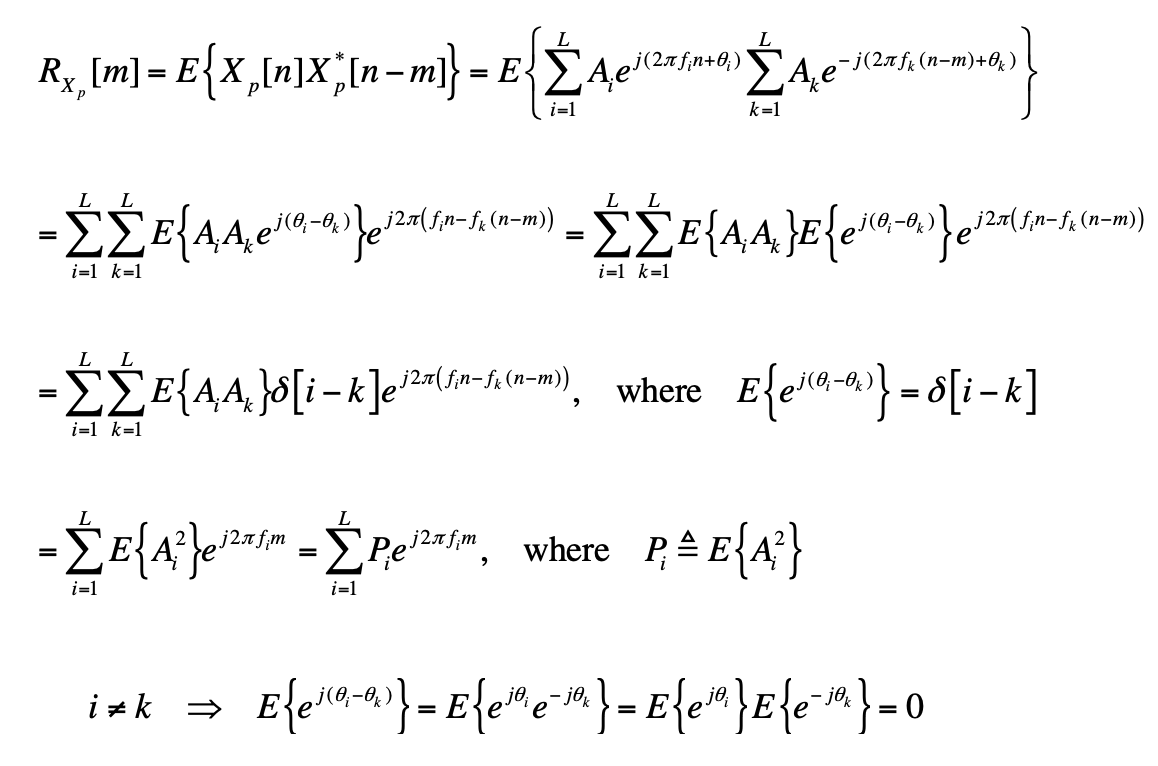
\includegraphics[width=0.65\linewidth]{Image/pdf 6/1.Formule.png}
    \label{fig:placeholder}
\end{figure}
\vspace{-3em}
\begin{align*}
S_X(z)
&= \sum_{m=-\infty}^{+\infty} R_X[m] z^{-m}
 = \sum_{m=-\infty}^{+\infty}
   \left(R_X^{c}[m] + \sum_{i=1}^{L} P_i e^{j2\pi f_i m}\right) z^{-m} \\[4pt]
&= \sum_{m=-\infty}^{+\infty} R_X^{c}[m] z^{-m}
 + \sum_{m=-\infty}^{+\infty}\sum_{i=1}^{L} P_i e^{j2\pi f_i m} z^{-m} \\[4pt]
&= \sum_{m=-\infty}^{+\infty} R_X^{c}[m] z^{-m}
 + \sum_{i=1}^{L} P_i \sum_{m=-\infty}^{+\infty}
   \big(e^{j2\pi f_i} z^{-1}\big)^{m} \\[4pt]
&= S_X^{c}(z)
 + \sum_{i=1}^{L} 2\pi P_i\,\delta\!\big(z - e^{j2\pi f_i}\big),
\end{align*}

\item Hence, \underline{the lines in the spectrum are generated by the periodic components in the ACF, which}\\ \underline{in turn are generated by the periodic components in the realizations of the random process}.
\item \textbf{Example}: cosinusoidal process in AWGN.
\[
X[n] = S[n] + W[n]
     = A\cos\big(2\pi f_{0} n + \theta_{0}\big) + W[n],
\qquad 0 < f_{0} < \tfrac{1}{2}
\]

\item The amplitude \(A\) is modelled as a Rayleigh r.v., the phase \(\theta_0\) is modelled as a r.v. uniformly distributed in \([-\pi,+\pi)\).
\[
A \in \mathcal{R}(\sigma_{A}^{2}), 
\qquad \theta_{0} \sim \mathcal{U}(-\pi,\pi),
\qquad A \text{ and } \theta_{0} \text{ independent},
\]

\[
f_{A}(a) = \frac{a}{\sigma_{A}^{2}} e^{-\frac{a^{2}}{2\sigma_{A}^{2}}} u(a),
\qquad
E\{A^{2}\} = 2\sigma_{A}^{2},
\]

\[
R_{X}[m] = E\{X[n]X[n+m]\}
        = R_{S}[m] + R_{W}[m]
        = \sigma_{A}^{2}\cos(2\pi f_{0} m) + \sigma_{W}^{2}\delta[m].
\]
\begin{align*}
S_X\!\left(e^{j2\pi f}\right)
&= 2\pi \frac{\sigma_{A}^{2}}{2}\,
   \delta\!\left(e^{j2\pi f} - e^{j2\pi f_{0}}\right)
 + 2\pi \frac{\sigma_{A}^{2}}{2}\,
   \delta\!\left(e^{j2\pi f} - e^{-j2\pi f_{0}}\right)
 + \sigma_{W}^{2}
\end{align*}
\[
S_X(z)
= \underbrace{2\pi \frac{\sigma_{A}^{2}}{2}\,
   \delta\!\left(z - e^{j2\pi f_{0}}\right)
 + 2\pi \frac{\sigma_{A}^{2}}{2}\,
   \delta\!\left(z - e^{-j2\pi f_{0}}\right)}_{\text{Discrete part}}
 + \underbrace{\sigma_{W}^{2}}_{\text{Continuous part}}
\]
\item Hence, \(W[n]\) is the regular part, whereas \(S[n]\) is the predictable part of \(X[n]\).
\begin{align*}
E\{S^{2}[n]\}
&= R_{S}[0]
 = \int_{-1/2}^{1/2}
   \left[
      2\pi\frac{\sigma_{A}^{2}}{2}
      \,\delta\!\left(e^{j2\pi f} - e^{j2\pi f_{0}}\right)
    + 2\pi\frac{\sigma_{A}^{2}}{2}
      \,\delta\!\left(e^{j2\pi f} - e^{-j2\pi f_{0}}\right)
   \right] df \\[4pt]
&= 2 \int_{0}^{1/2}
   2\pi\frac{\sigma_{A}^{2}}{2}
   \,\delta\!\left(e^{j2\pi f} - e^{j2\pi f_{0}}\right) df = \sigma_{A}^{2}\int_{0}^{\pi}
   \delta\!\left(e^{j\omega} - e^{j\omega_{0}}\right) d\omega
 = \sigma_{A}^{2}.
\end{align*}
\[
X[n] = X_{r}[n] + X_{p}[n]
     = X_{r}[n] + \sum_{i=1}^{L} A_{i} e^{j(2\pi f_{i} n + \theta_{i})}
\]
\vspace{-1em}
\[
R_{X}[m]
= R_{X}^{c}[m] + \sum_{i=1}^{L} P_{i} e^{j2\pi f_{i} m},
\qquad
\text{where } R_{X}^{c}[m] = ACF\{X_{r}[n]\},\;
P_{i} = E\{A_{i}^{2}\} = ACF\{X_{p}[n]\}.
\]
\vspace{-1em}
\[
S_{X}\!\left(e^{j2\pi f}\right)
= S_{X}^{c}\!\left(e^{j2\pi f}\right)
  + \sum_{i=1}^{L} 2\pi P_{i}\,
    \delta\!\left(e^{j2\pi f} - e^{j2\pi f_{i}}\right),
\qquad
\text{where } S_{X}^{c}(e^{j2\pi f}) = PSD\{X_{r}[n]\}.
\]

\item \textbf{Predictable} component \(X_p[n]\) corresponds to the discrete part of the PSD.
\item The \textbf{regular} component \(X_r[n]\) corresponds to the continuous part of the PSD.
\item A \textbf{white process} is a \textbf{regular} process, its PSD is continuous and constant:
\[
S_X^c
(e^{j2\pi f})=\sigma^2
\]
\item It is a \textbf{parametric model} that depends on only 1 parameter, that is the power of the process \(\sigma^2\). Once we know (estimate) \(\sigma^2\) we know the PSD:

\item \textbf{\underline{Problem}: How to model parametrically a non-white \textbf{regular process}}?
\item if the continuous part of the PSD satisfies the \textbf{Paley-Wiener condition} for discrete-time random processes:
\[
\int_{-1/2}^{1/2} \Big |\ln S_X^c (e^{j2\pi f})\Big |<+\infty
\]
\item then, the \textbf{regular} part of \(X[n]\) can be represented as the output of a linear time-invariant (LTI) filter with system function \(L(z)\), causal and stable, called the \textbf{innovation filter} with inverse \(\Gamma (z)=1/L(z)\), that is also causal and stable, called the \textbf{whitening filter}, having at the input a white process \(W[n]\), called the \textbf{innovation process}.

\item A \textbf{regular} process \(X[n]\) whose PSD satisfies the Paley-Wiener condition can be represented as follows:
\begin{figure}[H]
    \centering
    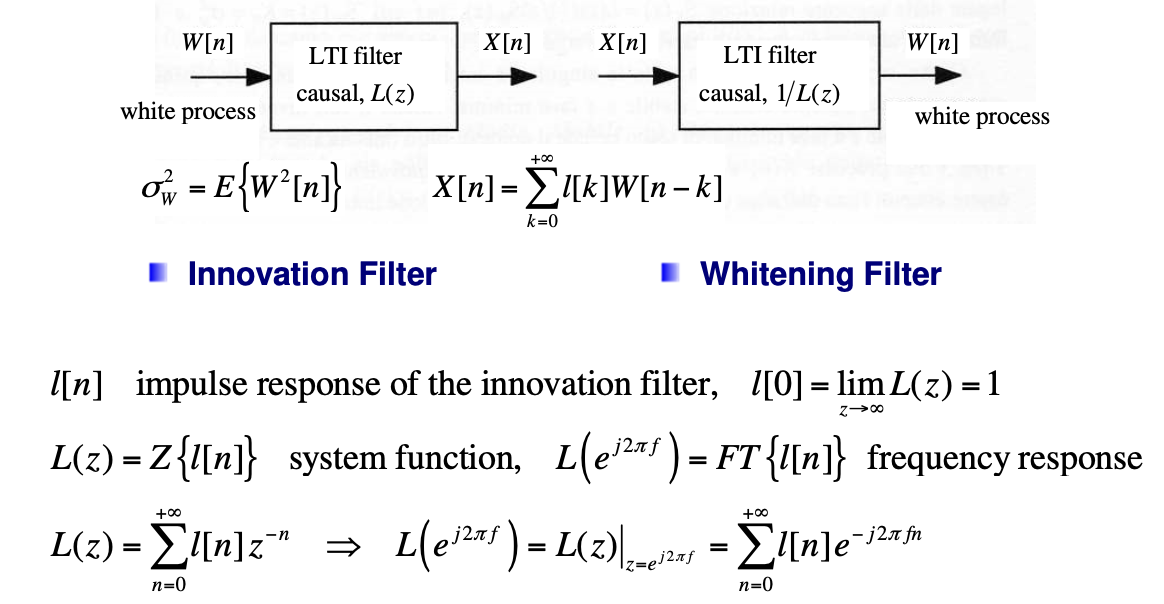
\includegraphics[width=0.75\linewidth]{Image/pdf 6/2.Filter.png}
    \label{fig:placeholder}
\end{figure}
\begin{figure}[H]
    \centering
    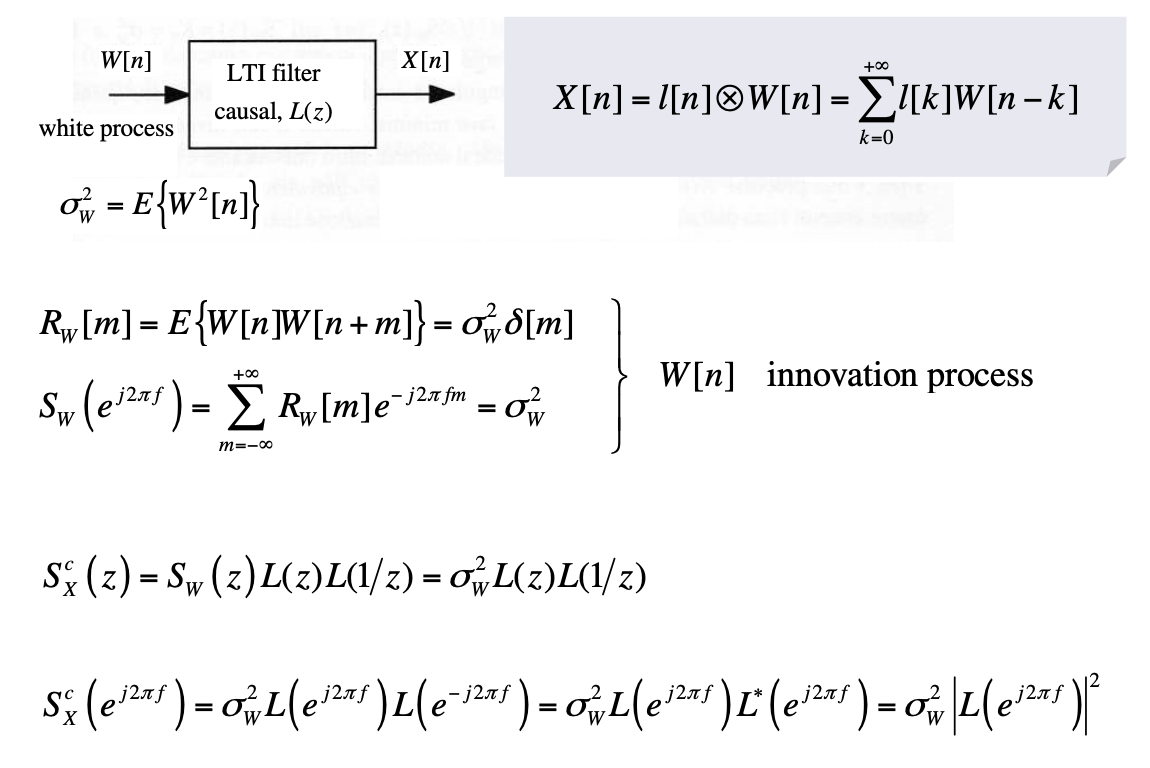
\includegraphics[width=0.75\linewidth]{Image/pdf 6/3.filter.png}
    \label{fig:placeholder}
\end{figure}
\begin{figure}[H]
    \centering
    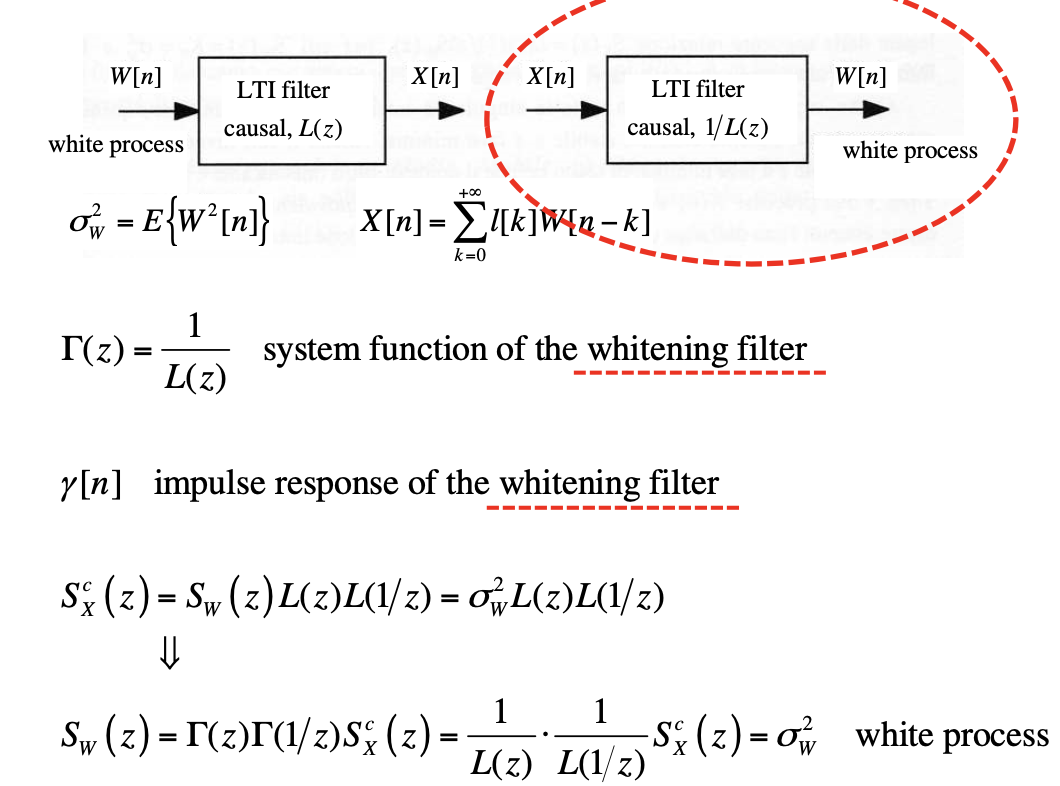
\includegraphics[width=0.75\linewidth]{Image/pdf 6/4.Filter.png}
    \label{fig:placeholder}
\end{figure}
\end{itemize}
\subsubsection{Signal with rational spectra}
\begin{itemize}
    \item According to the \textbf{Weistrass theorem}, the complex PSD of a WSS \textbf{regular} process can be always represented as the ratio of polynomials of proper orders (as a limit the order can be infinity):
\[
S_{X}(z)
= \sigma_{W}^{2} L(z)L\!\left(\frac{1}{z}\right)
= \sigma_{W}^{2} \frac{B(z)B\!\left(\frac{1}{z}\right)}
                      {A(z)A\!\left(\frac{1}{z}\right)},
\qquad
r_{1} < |z| < \frac{1}{r_{1}}
\]

    \item Where \(A(z)\) and \(B(z)\) are polynomials with all roots internal to the unit circle.
    \item The ROC is annular and it is determined by the dominant pole, i.e. the pole closest to the unit circle: if the dominant pole is \(p_1=r_1\exp(j\phi_1)\) and \(r_1\) is the modulo of this pole, the ROC is as above.
    \item A PSD of this kind always satisfies the Paley-Wiener condition.
    \item \textbf{Innovation filter}: causal stable,minimum phase, with inverse (the \textbf{whitening filter}) causal, stable and minimum phase.
    \[
L(z) = \frac{B(z)}{A(z)}
     = \frac{\displaystyle\sum_{k=0}^{Q} b_{k} z^{-k}}
            {\displaystyle 1 - \sum_{k=1}^{P} a_{k} z^{-k}},
\qquad r_{1} < |z|
\]

\[
\Gamma(z) = \frac{1}{L(z)} = \frac{A(z)}{B(z)}
\]

\[
X[n] = l[n] \otimes W[n]
     = \sum_{k=0}^{+\infty} l[k]\,W[n-k]\qquad l[0] = \lim_{z\to\infty} L(z) = b_{0} = 1,
\]

\[
W[n] = \gamma[n] \otimes X[n]
     = \sum_{k=0}^{+\infty} \gamma[k]\,X[n-k]\qquad\gamma[0] = \lim_{z\to\infty} \frac{1}{L(z)} = 1
\]

    \item The input-output relationship of the \textbf{innovation filter} in the time-domain can be obtained as follows:
    \[
X(z) = L(z)W(z)
     = \frac{B(z)}{A(z)} W(z)
     = \frac{\displaystyle\sum_{k=0}^{Q} b_{k} z^{-k}}
            {\displaystyle 1 - \sum_{k=1}^{P} a_{k} z^{-k}}\, W(z)
\]

\[
\left(1 - \sum_{k=1}^{P} a_{k} z^{-k}\right) X(z)
 = \left(\sum_{k=0}^{Q} b_{k} z^{-k}\right) W(z)
 \;\Longrightarrow\;
 X(z) = \sum_{k=1}^{P} a_{k} z^{-k} X(z) + \sum_{k=0}^{Q} b_{k} z^{-k} W(z)
\]
\item Calculating the inverse Z-transform, we get the \textit{input-output} relationship in the time-domain:


\[
X[n]=\sum_{k=1}^{P}a_kX[n-k]+\sum_{k=0}^{Q}b_kW[n-k]
\]
\item Processes of this kind, whose \textit{input-output} relationship is described by a recursive linear difference equation with constant coefficients, are called \textbf{Atuoregressive Moving Average} processes of order (P,Q):\textbf{Arma (P,Q)}
\begin{figure}[H]
    \centering
    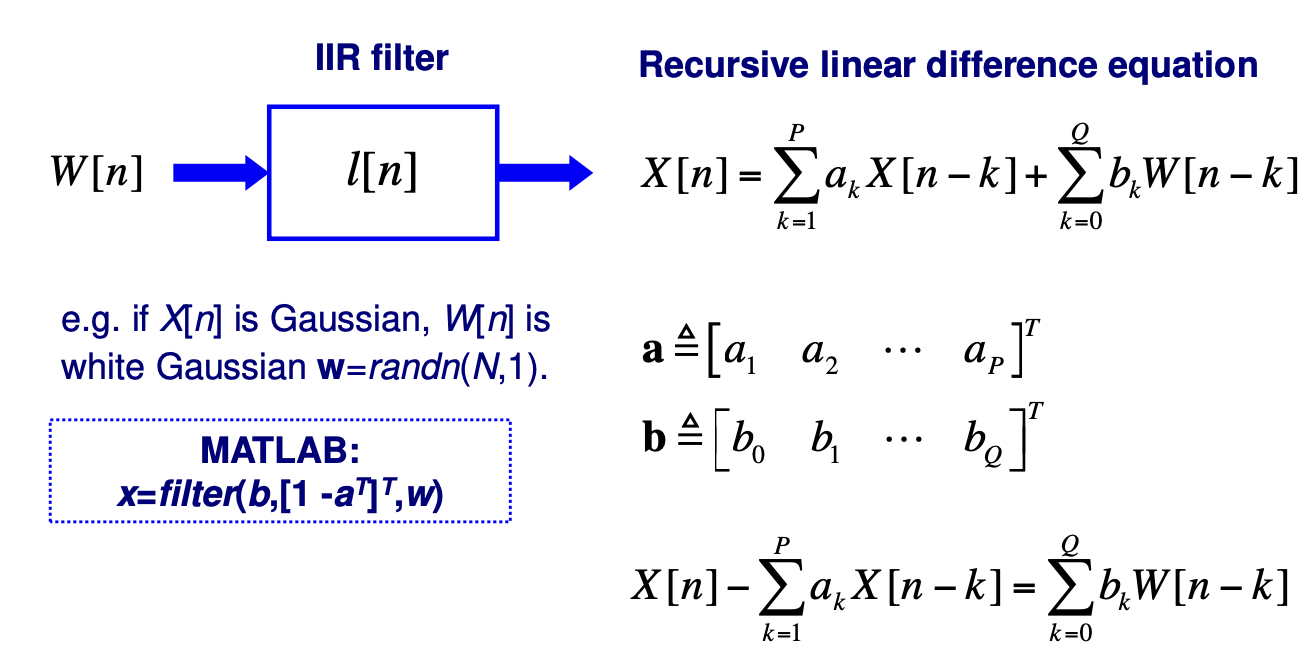
\includegraphics[width=0.75\linewidth]{Image/pdf 6/5.Filter_schem.png}
    \label{fig:placeholder}
\end{figure}
\item \textbf{IMPORTANT}: Any regular process that satisfies the Paley-Wiener condition can be modelled as an \textbf{Arma(P,Q)}, process with orders \textit{P} and/or \textit{Q} possibly infinite.
\[
\text{System function:}\qquad
L(z) = \frac{B(z)}{A(z)}
     = \frac{\displaystyle\sum_{k=0}^{Q} b_{k} z^{-k}}
            {\displaystyle 1 - \sum_{k=1}^{P} a_{k} z^{-k}}
\]
\vspace{-1em}
\[
\text{Frequency response:}\qquad
L\!\left(e^{j2\pi f}\right)
  = L(z)\big|_{z=e^{j2\pi f}}
  = \frac{B\!\left(e^{j2\pi f}\right)}
         {A\!\left(e^{j2\pi f}\right)}
  = \frac{\displaystyle\sum_{k=0}^{Q} b_{k} e^{-j2\pi k f}}
         {\displaystyle 1 - \sum_{k=1}^{P} a_{k} e^{-j2\pi k f}}
\]
\[
\text{Complex PSD:}\qquad
S_{X}(z)
= \sigma_{W}^{2} L(z)L(1/z)
= \sigma_{W}^{2}
  \left(
    \frac{\displaystyle\sum_{k=0}^{Q} b_{k} z^{-k}}
         {\displaystyle 1 - \sum_{k=1}^{P} a_{k} z^{-k}}
  \right)
  \left(
    \frac{\displaystyle\sum_{k=0}^{Q} b_{k} z^{k}}
         {\displaystyle 1 - \sum_{k=1}^{P} a_{k} z^{k}}
  \right)
\]

\[
\text{PSD:}\qquad
S_{X}\!\left(e^{j2\pi f}\right)
= \sigma_{W}^{2}\bigl|L(e^{j2\pi f})\bigr|^{2}
= \sigma_{W}^{2}
  \left|
    \frac{\displaystyle\sum_{k=0}^{Q} b_{k} e^{-j2\pi k f}}
         {\displaystyle 1 - \sum_{k=1}^{P} a_{k} e^{-j2\pi k f}}
  \right|^{2}
\]

\[
S_{X}\!\left(e^{j2\pi f}\right)
\;\Longleftrightarrow\;
\bigl\{\sigma_{W}^{2},\mathbf{a},\mathbf{b}\bigr\}
\quad\Rightarrow\quad
P+Q+1\ \text{parameters}\ \ (\text{if } b_{0}=1)
\]

\[
\mathbf{a} \triangleq [a_{1}\; a_{2}\; \dots\; a_{P}]^{T},
\qquad
\mathbf{b} \triangleq [b_{1}\; b_{2}\; \dots\; b_{Q}]^{T}
\]
\[
L(z)
= \frac{\displaystyle\sum_{k=0}^{Q} b_{k} z^{-k}}
       {\displaystyle 1 - \sum_{k=1}^{P} a_{k} z^{-k}}
= \frac{z^{-Q}\displaystyle\sum_{k=0}^{Q} b_{k} z^{Q-k}}
       {z^{-P}\Bigl[z^{P} - \displaystyle\sum_{k=1}^{P} a_{k} z^{P-k}\Bigr]}
= z^{P-Q}\,
  \frac{\displaystyle\sum_{k=0}^{Q} b_{k} z^{Q-k}}
       {\displaystyle z^{P} - \sum_{k=1}^{P} a_{k} z^{P-k}}
\]

\[
= z^{P-Q}\,
  \frac{b_{0} z^{Q} + b_{1} z^{Q-1} + \cdots + b_{Q-1} z + b_{Q}}
       {z^{P} - a_{1} z^{P-1} - \cdots - a_{P-1} z - a_{P}}
= b_{0} z^{P-Q}\,
  \frac{z^{Q} + \dfrac{b_{1}}{b_{0}} z^{Q-1} + \cdots + \dfrac{b_{Q}}{b_{0}}}
       {z^{P} - a_{1} z^{P-1} - \cdots - a_{P}}
\]

\[
= b_{0} z^{P-Q}\,
  \frac{\displaystyle\prod_{n=1}^{Q} (z - z_{n})}
       {\displaystyle\prod_{n=1}^{P} (z - p_{n})}
\]
\noindent \item \textbf{Poles of the filter= roots of the characteristic equation}
\[
z^P-a_1z^{P-1}-...-a_{P-1}z-a_P=0
\]
\[
L\!\left(e^{j2\pi f}\right)
= b_{0}\, e^{j2\pi f (P-Q)}
  \frac{\displaystyle\prod_{n=1}^{Q}\bigl(e^{j2\pi f} - z_{n}\bigr)}
       {\displaystyle\prod_{n=1}^{P}\bigl(e^{j2\pi f} - p_{n}\bigr)}
\]

\item The behavior of the \textbf{frequency response} of the \textbf{innovation filter} is a function of the coefficients \(\{a_k\}\) and \(\{b_k\}\) of the recursive equation, i.e. it is a function of the location of the \textbf{poles} and \textbf{zeros} of the innovation filter(func matlab stica).
\[
S_{X}\!\left(e^{j2\pi f}\right)
= \sigma_{W}^{2}\,\bigl|L(e^{j2\pi f})\bigr|^{2}
= \sigma_{W}^{2} b_{0}^{2}\,
  \frac{\displaystyle\prod_{n=1}^{Q}
        \bigl|e^{j2\pi f} - z_{n}\bigr|^{2}}
       {\displaystyle\prod_{n=1}^{P}
        \bigl|e^{j2\pi f} - p_{n}\bigr|^{2}}
\]
\vspace{-1em}
\[
\text{where}\qquad
\sigma_{W}^{2} = E\{W^{2}[n]\}
\]

\item Hence, also the behavior of the PSD (and so of the ACF) depends on the coefficients \(\{a_k\}\) and \(\{b_k\}\), i.e. on the location of the poles and zeros of the innovation filter.
\item Usually, we set \(l[0]=b_0=1\) to avoid ambiguity with the innovation power.
\item The shape of the PSD (and so of the ACF) is uniquely a function of the locations of the poles and zeros of the innovation filter.
\item The power of the innovation process is just a scale factor, it does not affect the PSD shape.

\[
S_{X}\!\left(e^{j2\pi f}\right)
\;\Longleftrightarrow\;
\bigl\{\sigma_{W}^{2},\mathbf{a},\mathbf{b}\bigr\}
\;\Longleftrightarrow\;
\bigl\{\sigma_{W}^{2} b_{0}^{2},\mathbf{p},\mathbf{z}\bigr\}
\]

\[
\mathbf{p} \triangleq [p_{1}\; p_{2}\; \dots\; p_{P}]^{T},
\qquad
\mathbf{z} \triangleq [z_{1}\; z_{2}\; \dots\; z_{Q}]^{T}
\]

\[
b_{0} = 1
\;\Longrightarrow\;
\bigl\{\sigma_{W}^{2},\mathbf{p},\mathbf{z}\bigr\}
\;\Rightarrow\;
P + Q + 1\ \text{parameters}
\]
\begin{figure}[H]
    \centering
    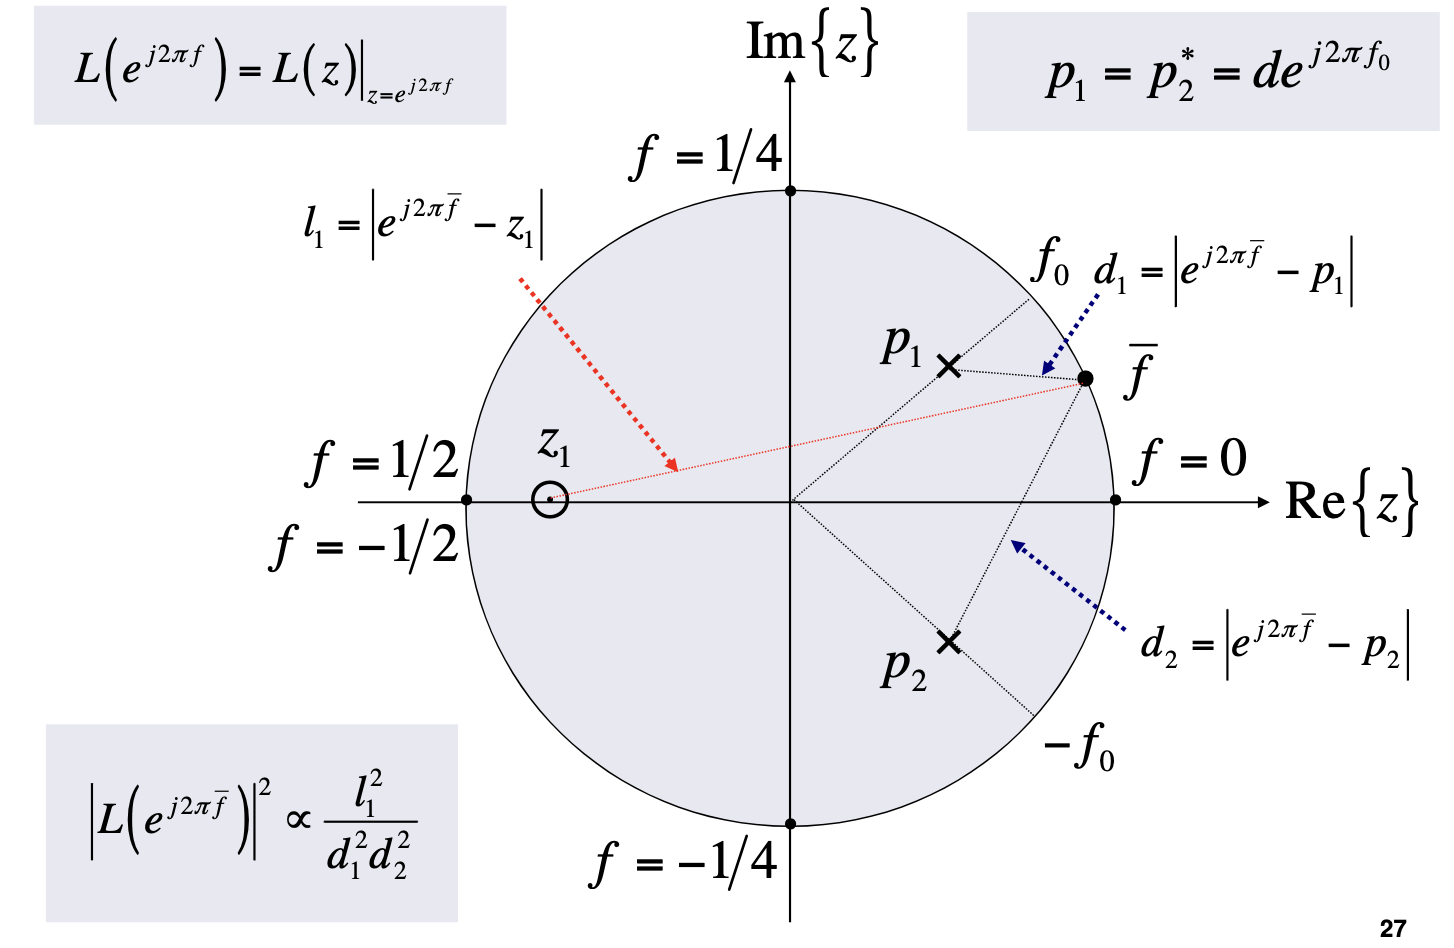
\includegraphics[width=0.65\linewidth]{Image/pdf 6/6.Roba_esb.png}
    \label{fig:placeholder}
\end{figure}
\item \textbf{Summary}:
    The shape of the PSD, and also of the ACF, is uniquely determined by the locations of the poles and zeros of the innovation filter \(L(z)\).\\
    The phases of the poles determine the frequencies where the peaks in the PSD are located. How much a peak is pronounced is determined by the modulo of the pole: the closer the pole is to the unit circle and the narrower the peak is.\\
    The phases of the zeros determine the frequencies where the valleys in the PSD are located. How much a valley is narrow is determined by the modulo of the zero: the closer the zero is to the unit circle and the narrower the valley is.\\
    In most of the cases, we are more interested on identifying the locations of the peaks and their widths rather than those of the valleys.    
\end{itemize}

\subsection{Autoregressive processes: AR(P)}
\begin{figure}
    \centering
    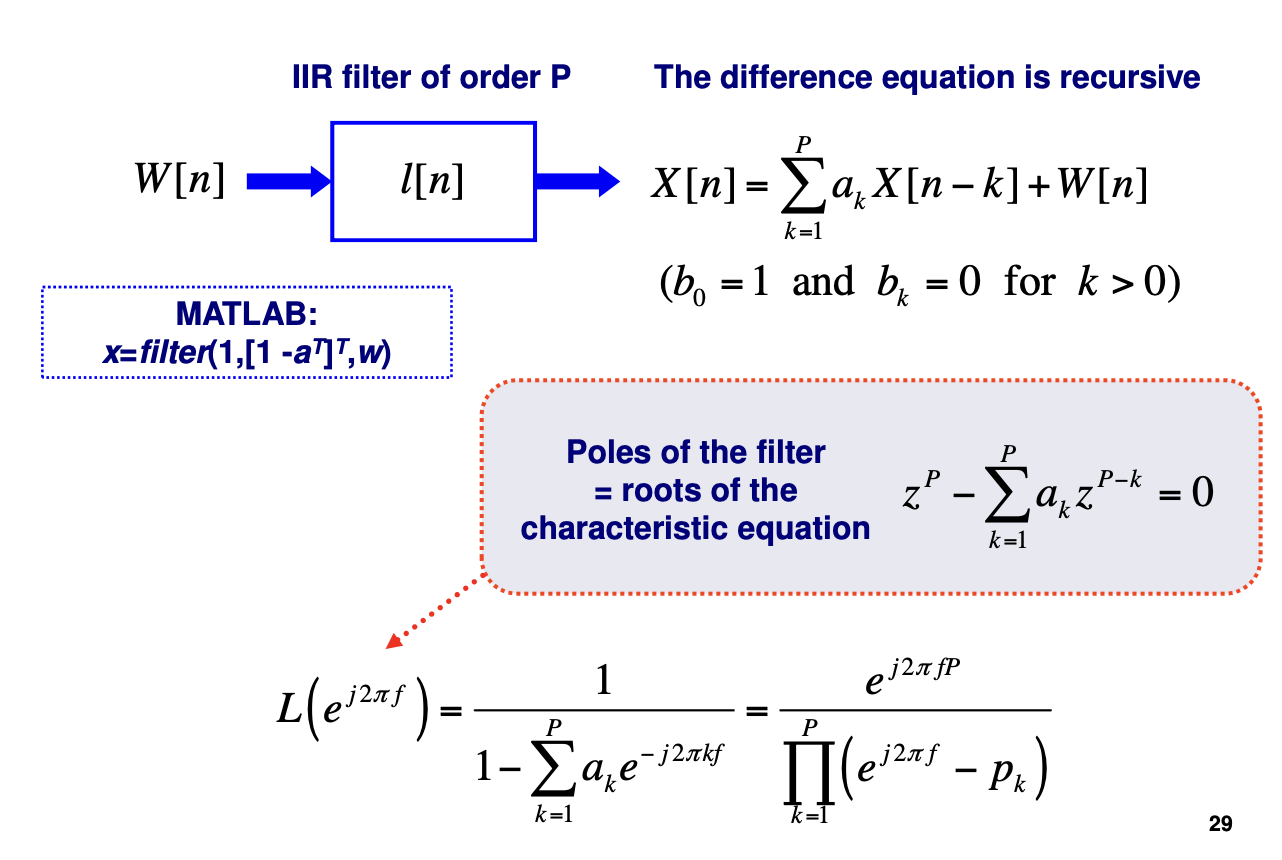
\includegraphics[width=0.75\linewidth]{Image/pdf 6/7.AR(P).png}
    \label{fig:placeholder}
\end{figure}
\noindent Lets study AR(1):
\[
X[n]=\rho X[n-1]+W[n]\qquad(a_1=\rho)\qquad\text{characteristic equation: } z-\rho=0
\]
\begin{align*}
&X(z) = \rho z^{-1} X(z) + W(z)
\;\Longrightarrow\;
\bigl(1 - \rho z^{-1}\bigr) X(z) = W(z)\\[4pt]
&L(z) = \frac{X(z)}{W(z)}
     = \frac{1}{1 - \rho z^{-1}}
     = \frac{z}{z - \rho},
\qquad |\rho| < 1\\[4pt]
&L\!\left(e^{j2\pi f}\right)
= L(z)\big|_{z = e^{j2\pi f}}
= \frac{1}{1 - \rho e^{-j2\pi f}}
\end{align*}

\begin{itemize}
    \item The impulse response of the innovation filter of an AR(1) process can be evaluated by solving the relevant linear difference equation with a Kronecker delta as input sequence:
    \[
l[n] = \rho\,l[n-1] + \delta[n], \quad l[-1]=0,\quad |\rho|<1
\]

\[
\Longrightarrow
\begin{cases}
l[0] = \rho\,l[-1] + \delta[0] = 1,\\[4pt]
l[1] = \rho\,l[0] + \delta[1] = \rho,\\[4pt]
l[2] = \rho\,l[1] + \delta[2] = \rho^{2},\\
\ \vdots \\[4pt]
l[n] = \rho\,l[n-1] + \delta[n] = \rho^{n}
\end{cases}
\]
\item Then, finally :
\[
l[n]=\rho^nu[n],\quad|\rho|<1
\]
\item The transfer function \(L(z)\) of the innovation filter can also be derived as the Z-transform of the impulse response:
\begin{align*}
R_{X}[m]
  &= E\{X[n] X[n+m]\} \\[4pt]
  &= E\{X[n]\bigl(\rho X[n+m-1] + W[n+m]\bigr)\} \\[4pt]
  &= E\{\rho X[n] X[n+m-1]\} + E\{X[n] W[n+m]\} \\[4pt]
  &= \rho R_{X}[m-1]
\end{align*}

\[
\text{infatti}\quad E\{X[n] W[n+m]\} = 0 \quad \text{se } m>0
\]

\begin{align*}
R_{X}[m] - \rho R_{X}[m-1] &= 0, \qquad m>0 \\[4pt]
R_{X}[m] &= R_{X}[0]\rho^{m}, \qquad m>0
\end{align*}


\item \textbf{Autocorrelation function (ACF)} of an AR(1) process:
\begin{align*}
L(z)
  &= \sum_{n=0}^{+\infty} \rho^{n} z^{-n}
   = \sum_{n=0}^{+\infty} \bigl(\rho z^{-1}\bigr)^{n}
   = \frac{1}{1 - \rho z^{-1}}, \\[4pt]
|\rho z^{-1}| &< 1 \;\Longrightarrow\; |z| > |\rho|
\end{align*}

\item To derive \(R_X[0]\):
\begin{align*}
\sigma_{x}^{2}
  &= R_{X}[0]
   = E\{X^{2}[n]\}
   = E\bigl\{(\rho X[n-1] + W[n])^{2}\bigr\} \\[4pt]
  &= \rho^{2} E\{X^{2}[n-1]\}
   + 2\rho E\{X[n-1] W[n]\}
   + E\{W^{2}[n]\} \\[4pt]
  &= \rho^{2} \sigma_{x}^{2} + \sigma_{w}^{2}\quad\Longrightarrow\quad\sigma_{x}^{2}
  = \frac{\sigma_{w}^{2}}{1 - \rho^{2}}
\end{align*}
\item Taking into account that \(R_X[-m]=R_X[m]\)
\[
R_X[m]=\frac{\sigma_W^2}{1-\rho^2}\rho^{|m|}
\]

\begin{align*}
\rho_{X[n],X[n+m]}
  &= \frac{\operatorname{cov}\{X[n],X[n+m]\}}
          {\sqrt{\operatorname{var}\{X[n]\}\,\operatorname{var}\{X[n+m]\}}}
   = \frac{C_{X}[m]}{C_{X}[0]}
   = \frac{R_{X}[m]}{R_{X}[0]}
   = \rho^{|m|}
\end{align*}
\begin{figure}[H]
    \centering
    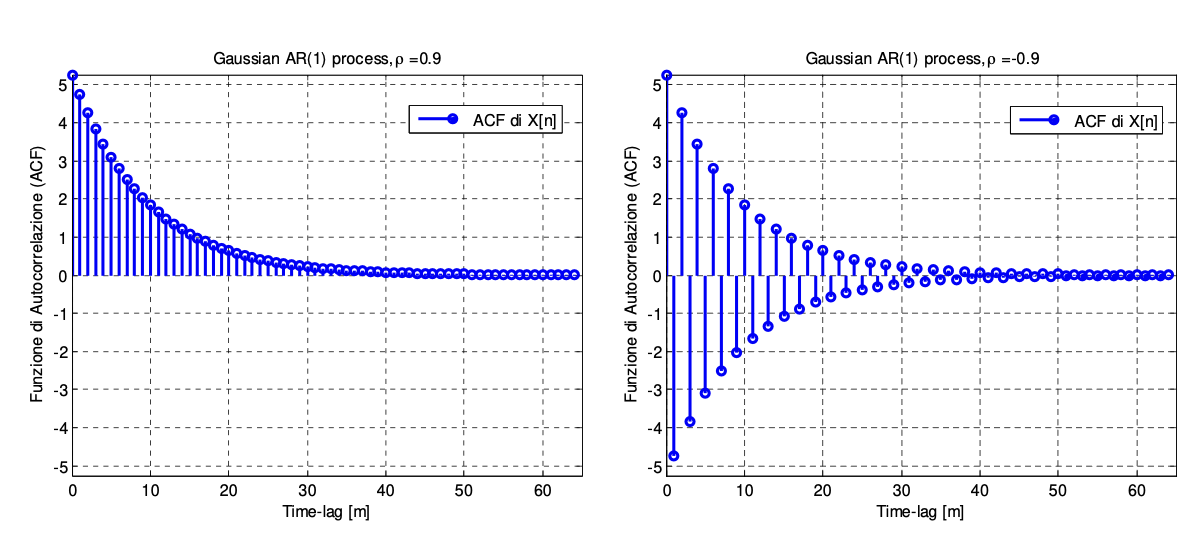
\includegraphics[width=0.65\linewidth]{Image/pdf 6/8.Graph_1.png}
    \label{fig:placeholder}
\end{figure}

\item The duration of the ACF (\textbf{correlation time} or \textbf{coherence time}) is larger when \(|\rho|\) is closer to the unit circle.
\begin{figure}[H]
    \centering
    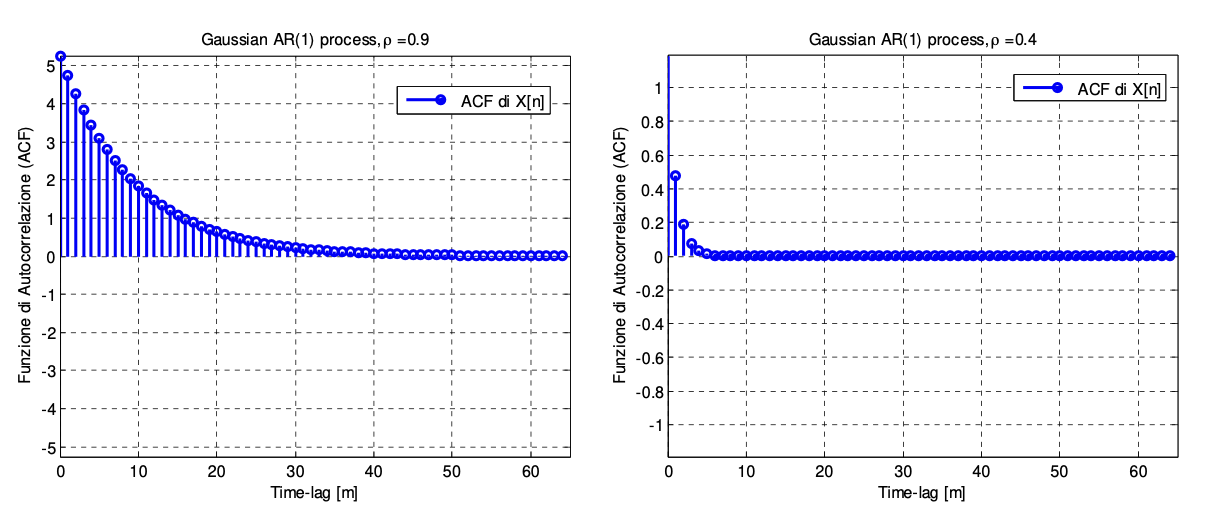
\includegraphics[width=0.65\linewidth]{Image/pdf 6/9.Graph_2.png}
    \label{fig:placeholder}
\end{figure}
\begin{align*}
S_{X}\!\left(e^{j2\pi f}\right)
  &= \sigma_{W}^{2}\bigl|L(e^{j2\pi f})\bigr|^{2}
   = \sigma_{W}^{2}\left|\frac{1}{1-\rho e^{-j2\pi f}}\right|^{2}
  = \frac{\sigma_{W}^{2}}{1 + \rho^{2} - 2\rho\cos(2\pi f)}
\end{align*}

\begin{figure}[H]
    \centering
    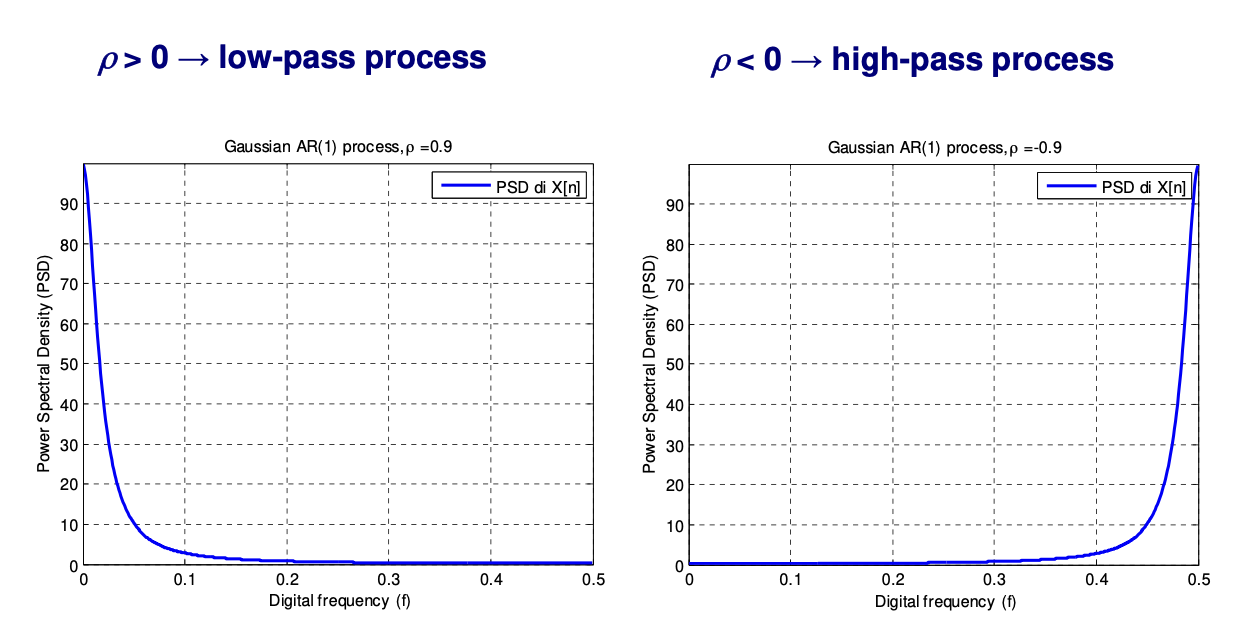
\includegraphics[width=0.65\linewidth]{Image/pdf 6/12.LP_HP.png}
    \label{fig:placeholder}
\end{figure}
\item With an AR(1) model we can obtain/represent only low-pass or high processes, but not pass-band process.
\item The bandwidth \(B\) of the process depend on how close the pole is to the unit circle: \(B\) gets lower when \(\rho\) gets closer to the unit circle.
\begin{figure}[H]
    \centering
    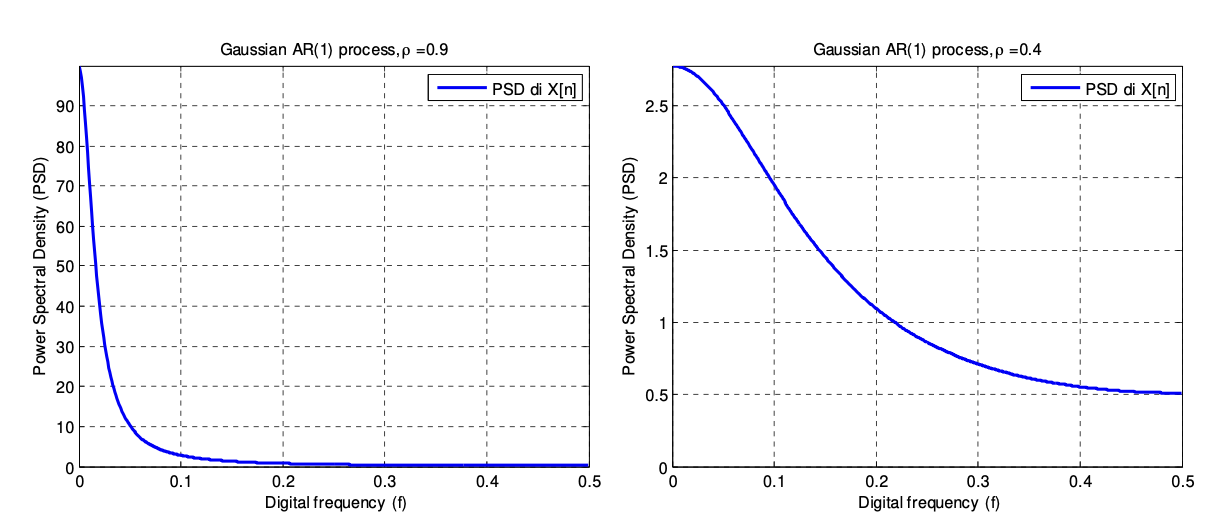
\includegraphics[width=0.65\linewidth]{Image/pdf 6/13.PSD_LP_HP.png}
    \label{fig:placeholder}
\end{figure}
\[
\rho_{X[n],X[n+m]}=\rho^{|m|}\quad\Rightarrow\quad\rho_{X[n],X[n+1]}=\rho
\]
\item Parameter \(\rho\) the \textbf{one-lag correlation coefficient} of the process.
\begin{figure}[H]
    \centering
    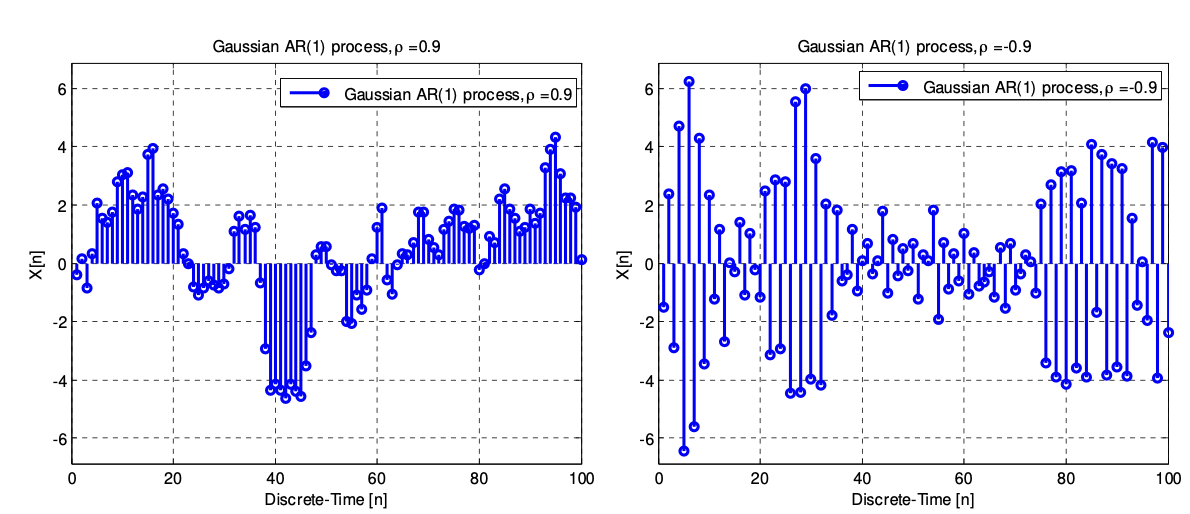
\includegraphics[width=0.65\linewidth]{Image/pdf 6/14.lag_corr.png}
    \label{fig:placeholder}
\end{figure}
\begin{figure}[H]
    \centering
    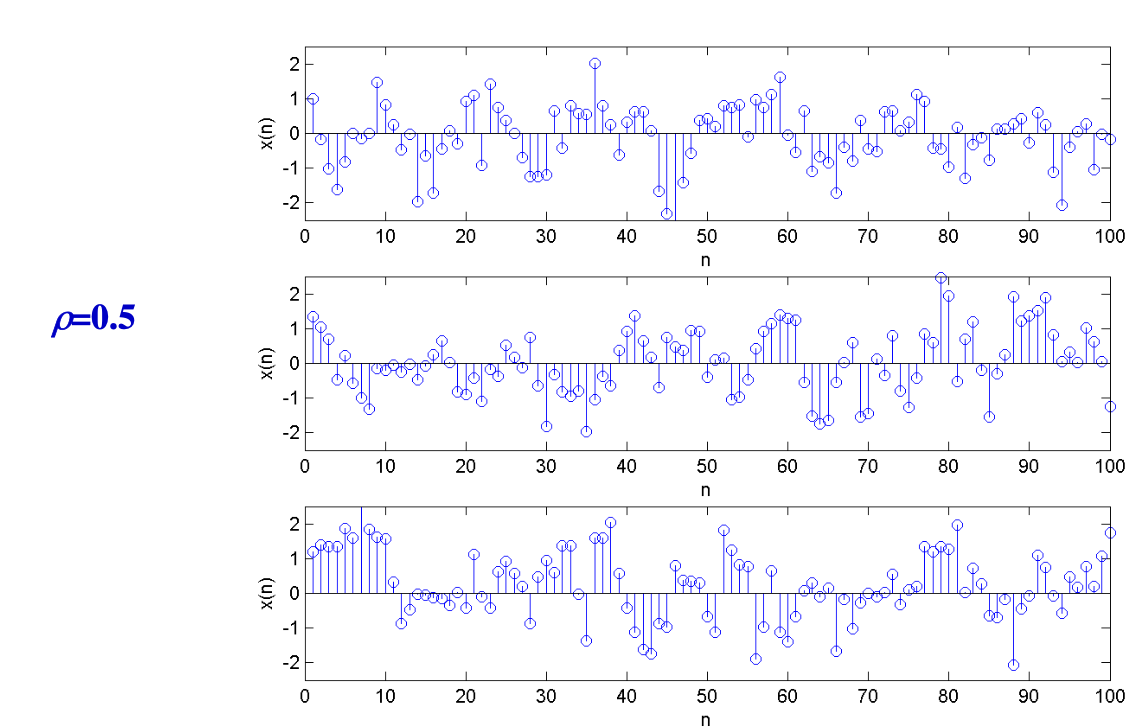
\includegraphics[width=0.65\linewidth]{Image/pdf 6/15.ex_rho_.png}
    \label{fig:placeholder}
\end{figure}
\begin{figure}[H]
    \centering
    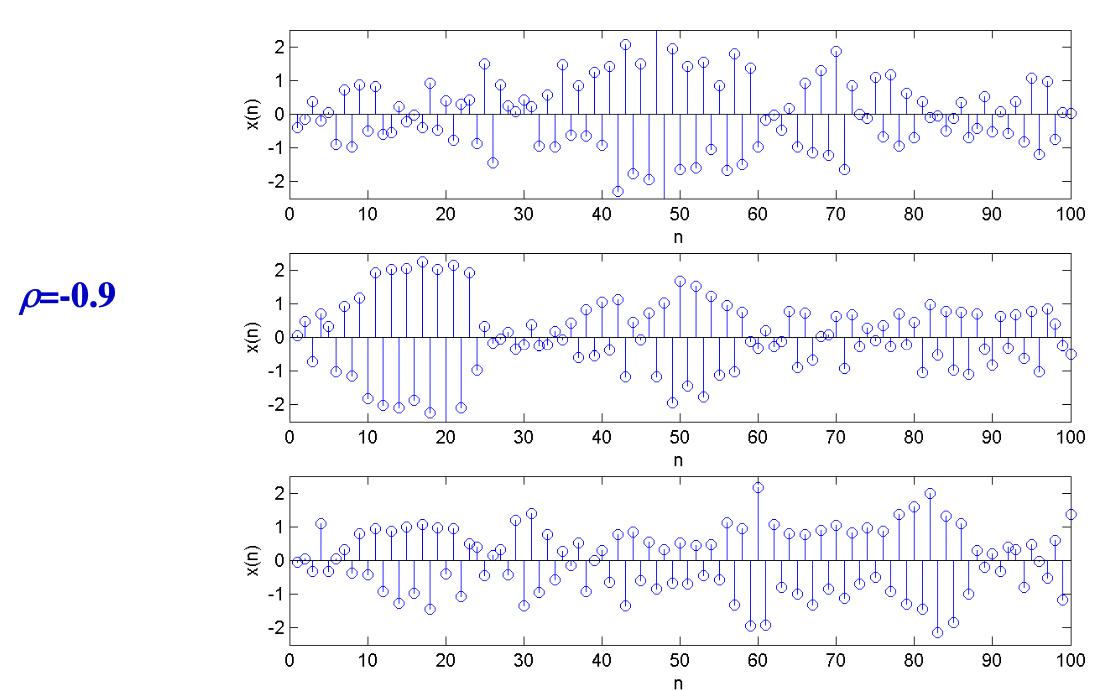
\includegraphics[width=0.65\linewidth]{Image/pdf 6/16.ex_corr_rho_2.png}
    \label{fig:placeholder}
\end{figure}
\begin{figure}
    \centering
    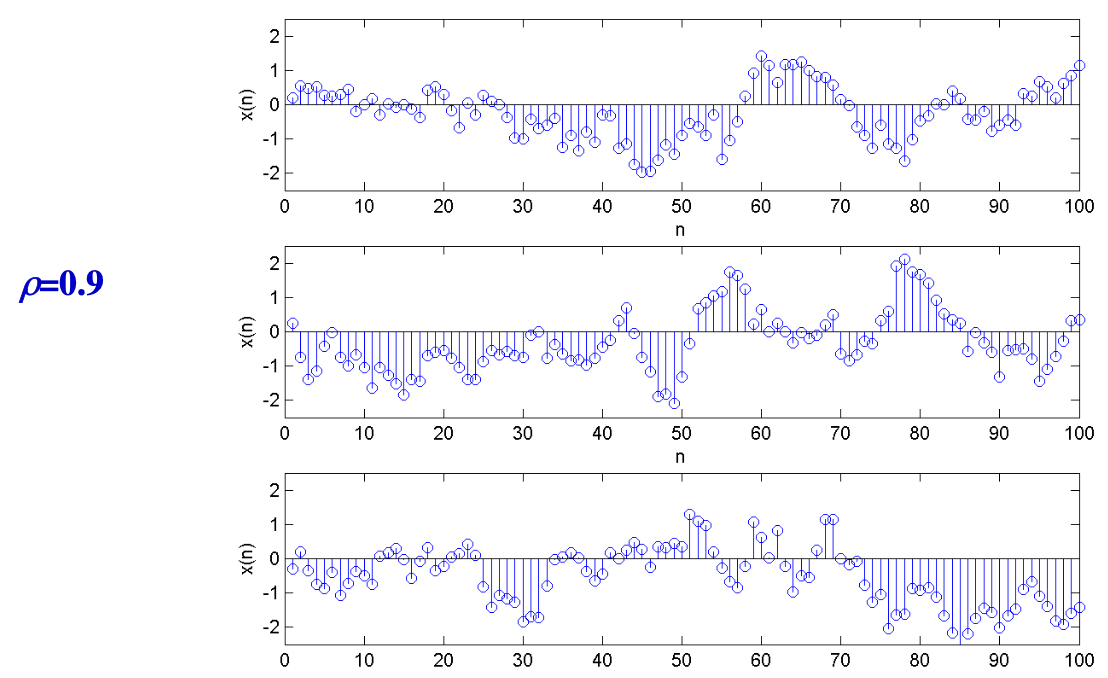
\includegraphics[width=0.65\linewidth]{Image/pdf 6/17.ex_corr_rho_3.png}
    \label{fig:placeholder}
\end{figure}
\end{itemize}
\subsubsection{AR(2) processes}
\begin{itemize}
    \item The PSD/ACF shape depends on the vector of parameters \textbf{a} and \textbf{b}, or equivalently on the pole and zeros locations.
    \item We have analyzed this in detail for an \textbf{AR(1)} process. We have seen that varying the value of the parameter \(a_1=\rho\) we can obtain a low-pass process (\(\rho>0\)) or an hig-pass process \((\rho<0)\), but we cannot ontain a pass-band process. The PSD bandwidth depeneds on \(|\rho|\).
    \item When the \(\rho=0\) we have the degenerate case \(X[n]=W[n]\), so process \(X[n]\) is white.
    \item Let us consider now an \textbf{AR(2) process} and let see how to obtain a \textbf{pass-band process} by properly selecting the values of \(a_1\) and \(a_2\), i.e. the location of the two poles \(p_1\) and \(p_2\).
    \[
    X[n]=a_1X[n-1]+a_2X[n-2]+W[n]
    \]
    \item Les us derive first the \textbf{system function} and \textbf{frequency response} of the \textbf{innovation filter}:
    \begin{align*}
X[n] &= a_{1} X[n-1] + a_{2} X[n-2] + W[n] \\[6pt]
X(z) &= a_{1} z^{-1} X(z) + a_{2} z^{-2} X(z) + W(z) \\[6pt]
L(z) &= \frac{X(z)}{W(z)}
     = \frac{1}{1 - a_{1} z^{-1} - a_{2} z^{-2}}
     = \frac{z^{2}}{z^{2} - a_{1} z - a_{2}} \\[6pt]
L\!\left(e^{j2\pi f}\right)
     &= \frac{1}{1 - a_{1} e^{-j2\pi f} - a_{2} e^{-j4\pi f}}
\end{align*}
\item The filter has 2 poles and 2 zeros at \(z=0\).
\item The poles are derived by solving the characteristic equation:
\[
z^2-a_1z-a_2=0\quad\Longrightarrow\quad p_{1,2}=\frac{a_1\pm\sqrt{a_1^2+4a_2}}{2}
\]
\item The complex PSD and the PSD can be immediately derived:
\begin{align*}
S_{X}(z)
  &= \sigma_{W}^{2}\,L(z)\,L\!\left(\frac{1}{z}\right) = \frac{\sigma_{W}^{2}}
          {\bigl(1-a_{1}z^{-1}-a_{2}z^{-2}\bigr)
           \bigl(1-a_{1}z-a_{2}z^{2}\bigr)} \\[6pt]
  &= \frac{\sigma_{W}^{2}}
          {\bigl(1-p_{1}z^{-1}\bigr)\bigl(1-p_{2}z^{-1}\bigr)
           \bigl(1-p_{1}z\bigr)\bigl(1-p_{2}z\bigr)},
           \qquad d<|z|<\frac{1}{d},\quad
           d=\max\{|p_{1}|,|p_{2}|\}
\end{align*}
\item The PSD of an AR(2) process with complex conjugate poles:
\[
p_1=p_2^*=de^{j2\pi f_0}
\]
\noindent is passband, with central frequency (close to) \(f_0\) and bandwidth \(B\) which depends on \(d\): the closer \(d\) is to 1 and the smaller \(B\) is.
\begin{figure}[H]
    \centering
    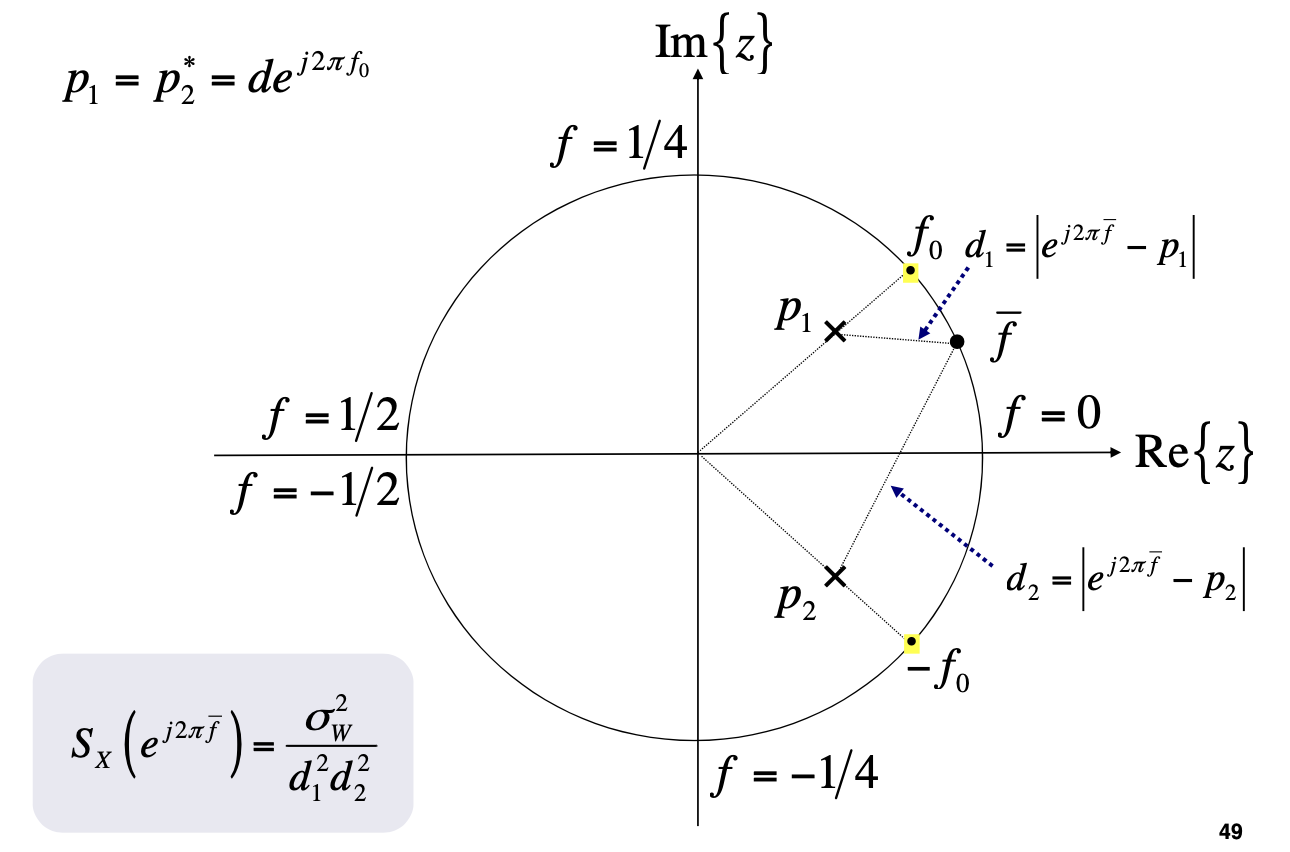
\includegraphics[width=0.65\linewidth]{Image/pdf 6/18.Poles_circle.png}
    \label{fig:placeholder}
\end{figure}
\item The \textbf{Autocorrelation function (ACF)} can be obtained by the inverse of the FFT of the PSD:
\[
R_X[m]=IFFT\{S_X(e^{j2\pi f})\}
\]
\item The ACF can also be obtained by solving the recursive equation derived for an AR(P) process in the following way:
\begin{align*}
P &= 2 \\[4pt]
R_{X}[m]
  &= \sum_{k=1}^{P} a_{k} R_{X}[m-k] + \sigma_{W}^{2}\delta[m],
      \qquad m \ge 0 \\[4pt]
R_{X}[m]
  &= a_{1} R_{X}[m-1] + a_{2} R_{X}[m-2] + \sigma_{W}^{2}\delta[m],
      \qquad m \ge 0
\end{align*}

\item Calculating it for \(m=0\) we get:
\[
R_X[0]=a_1R_X[-1]+a_2R_X[-2]+\sigma^2_W=a_1R_X[1]+a_2R_X[2]+\sigma^2_W
\]
\item If we now define the \textbf{normalized ACF}, which is the sequence of the correlation coefficients between \(X[n]\) and \(X[n+m]\) as a function of \(m\):
\begin{align*}
\rho_{X}[m]
  &\triangleq \frac{R_{X}[m]}{R_{X}[0]}
   = \frac{C_{X}[m]}{C_{X}[0]}
   = \frac{\operatorname{cov}\{X[n],X[n+m]\}}
          {\sqrt{\operatorname{var}\{X[n]\}\,\operatorname{var}\{X[n+m]\}}}
\end{align*}
\vspace{-0.5em}
\[
\Rightarrow\quad \rho_{X}[0] = 1
\]
\vspace{-1.5em}
\begin{align*}
R_{X}[0]
  &= a_{1} R_{X}[1] + a_{2} R_{X}[2] + \sigma_{W}^{2}= a_{1} R_{X}[0]\rho_{X}[1] + a_{2} R_{X}[0]\rho_{X}[2] + \sigma_{W}^{2}
\end{align*}
\item Thus, we get:
\[
R_X[0]=\frac{\sigma_W^2}{1-a_1\rho_X[1]-a_2\rho_X[2]}
\]

\item Calculating it for \(m>0\) we obtain the homogeneous difference equation:

\begin{align*}
R_{X}[m] - a_{1} R_{X}[m-1] - a_{2} R_{X}[m-2] &= 0, \qquad m>0 \\[6pt]
\rho_{X}[m] - a_{1} \rho_{X}[m-1] - a_{2} \rho_{X}[m-2] &= 0, \qquad m>0
\end{align*}


\item The solution of the difference equation for \(m>0\) is given by:
\begin{align*}
\rho_{X}[m] &=
\begin{cases}
C_{1} p_{1}^{m} + C_{2} p_{2}^{m}, & m>0,\ \text{if the poles are different},\\[4pt]
\left(C_{1} + m C_{2}\right) p_{1}^{m}, & m>0,\ \text{if the poles are coincident},
\end{cases}
\\[6pt]
&\text{Coincident poles} \iff \Delta = a_{1}^{2} + 4a_{2} = 0
\end{align*}
\item Taking into account that the ACF is an even function, e.g. for the case of different poles, we have:
\[
\rho_X[m]=C_1p_1^{|m|}+C_2p_2^{|m|}
\]
\item The two constants are obtained by imposing the initial conditions:
\[
\begin{cases}
\rho_{X}[0] = C_{1} + C_{2} = 1, \\[4pt]
\rho_{X}[1] = C_{1}p_{1} + C_{2}p_{2}
            = \frac{a_{1}}{1-a_{2}},
\end{cases}\]
\[
m=1 \quad \Longrightarrow \quad \rho_X[1]-a_1\rho_X[0]-a_2\rho_X[-1]=0 \quad \Longrightarrow\quad\rho_X[1]=\frac{a_1}{1-a_2}
\]
\item Solving the system of 2 linear equations we find the two constants:


\[
\begin{cases}
C_{1}=-\frac{1}{p_{2}-p_{1}}\!\left(\frac{a_{1}}{1-a_{2}}-p_{2}\right)
     =-\frac{1}{\sqrt{a_{1}^{2}+4a_{2}}}
       \left(\frac{a_{1}}{1-a_{2}}-\frac{a_{1}+\sqrt{a_{1}^{2}+4a_{2}}}{2}\right)\\
C_{2}= \frac{1}{p_{2}-p_{1}}\!\left(\frac{a_{1}}{1-a_{2}}-p_{1}\right)
     = \frac{1}{\sqrt{a_{1}^{2}+4a_{2}}}
       \left(\frac{a_{1}}{1-a_{2}}-\frac{a_{1}-\sqrt{a_{1}^{2}+4a_{2}}}{2}\right).
\end{cases}\]\vspace{0.5em}
\[
\hspace{-4.5em}p_{1} = \frac{a_{1}-\sqrt{a_{1}^{2}+4a_{2}}}{2},\quad 
p_{2} = \frac{a_{1}+\sqrt{a_{1}^{2}+4a_{2}}}{2},\quad\Rightarrow\quad
p_{2}-p_{1} = \frac{a_{1}+\sqrt{a_{1}^{2}+4a_{2}}}{2}
             -\frac{a_{1}-\sqrt{a_{1}^{2}+4a_{2}}}{2}
           = \sqrt{a_{1}^{2}+4a_{2}}.
\]
\item Once we have \(C_1\), \(C_2\) and \(\rho_X[m]\) we can obtain immediately \(R_X[0]\):
\[
R_X[0]=\frac{\sigma_W^2}{1-a_1\rho_X[1]-a_2\rho_X[2]}
\]
\item In the case o \textbf{complex poles}, since the coefficients of the characteristic equation \(a_1\) and \(a_2\) are real, the poles should be complex conjugated:
\[
\text{Complex conjugate poles} 
\;\;\Longleftrightarrow\;\;
\Delta = a_{1}^{2}+4a_{2} < 0
\]
\vspace{-0.5em}
\[
p_{1,2}
  = \frac{a_{1} \pm j\sqrt{-\left(a_{1}^{2}+4a_{2}\right)}}{2}
  = d\,e^{\pm j\omega_{0}}
  = d\,e^{\pm j2\pi f_{0}}
\]

\item In the case of complex conjugate poles, also the two constants \(C_1\) and \(C_2\) are complex conjugated:
\[
p_{1} = d e^{j2\pi f_{0}}, \qquad p_{2} = d e^{-j2\pi f_{0}}
\Rightarrow C_{1} = C e^{j\theta_{0}}, \qquad C_{2} = C e^{-j\theta_{0}}\]
\begin{align*}
\rho_{X}[m] &= C_{1} p_{1}^{|m|} + C_{2} p_{2}^{|m|}
           = C e^{j\theta_{0}} d^{|m|} e^{j2\pi f_{0}|m|}
             + C e^{-j\theta_{0}} d^{|m|} e^{-j2\pi f_{0}|m|}\\[4pt]
           &= 2 \Re\!\left\{ C e^{j\theta_{0}} d^{|m|} e^{j2\pi f_{0}|m|} \right\}
           = 2 C d^{|m|} \cos\!\bigl(2\pi f_{0}|m| + \theta_{0}\bigr)
\end{align*}
\item The constants \(C\) and \(\theta_0\) are obtained as the modulo and the phase of \(C_1\).
\item The ACF has an oscillatory behavior with period \(T_0=1/f_0\) which depends on the phases of the poles \(\pm2\pi f_0\). Whereas the envelope of the ACF tends to 0 with a speed that depends on the modulo \(d\) of the poles.
\begin{figure}[H]
    \centering
    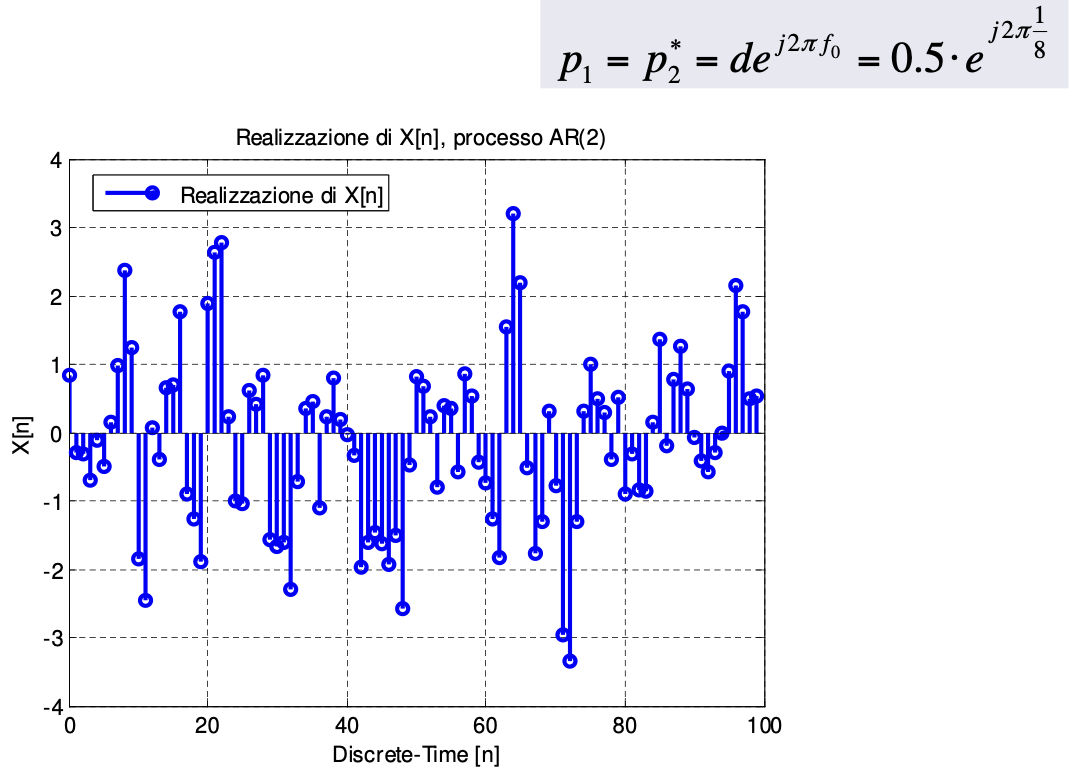
\includegraphics[width=0.65\linewidth]{Image/pdf 6/19.AR(2)_1.png}
    \label{fig:placeholder}
\end{figure}
\begin{figure}[H]
    \centering
    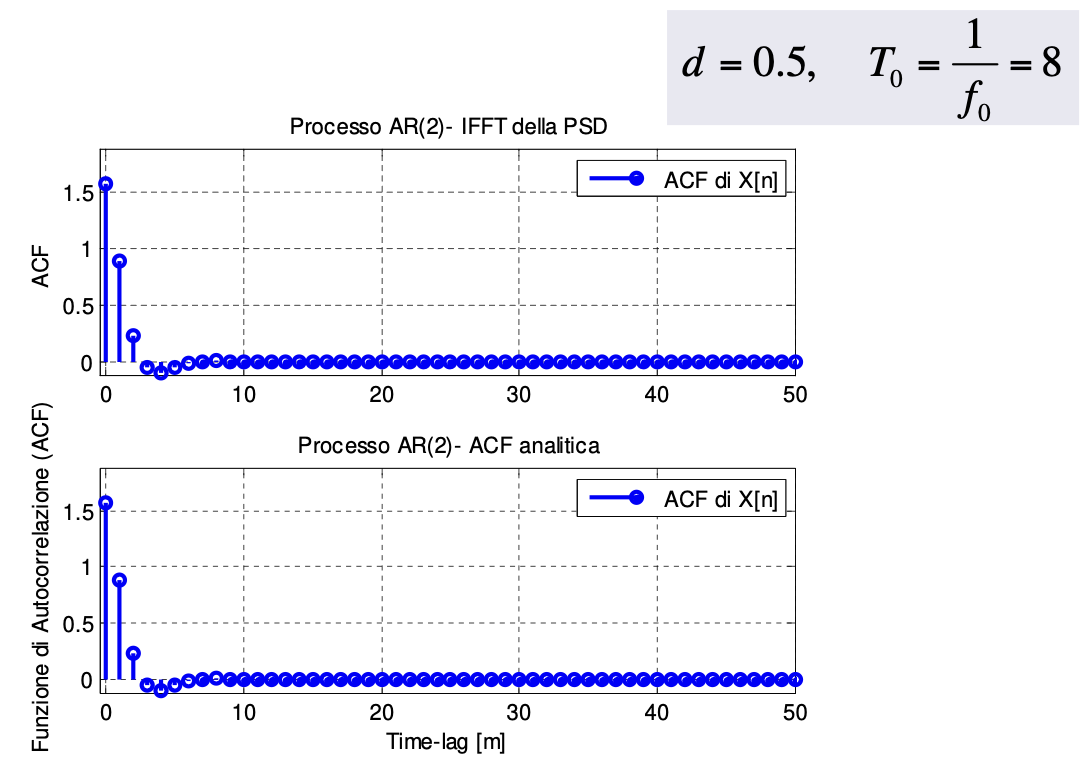
\includegraphics[width=0.65\linewidth]{Image/pdf 6/20.AR(2)_2.png}
    \label{fig:placeholder}
\end{figure}
\begin{figure}[H]
    \centering
    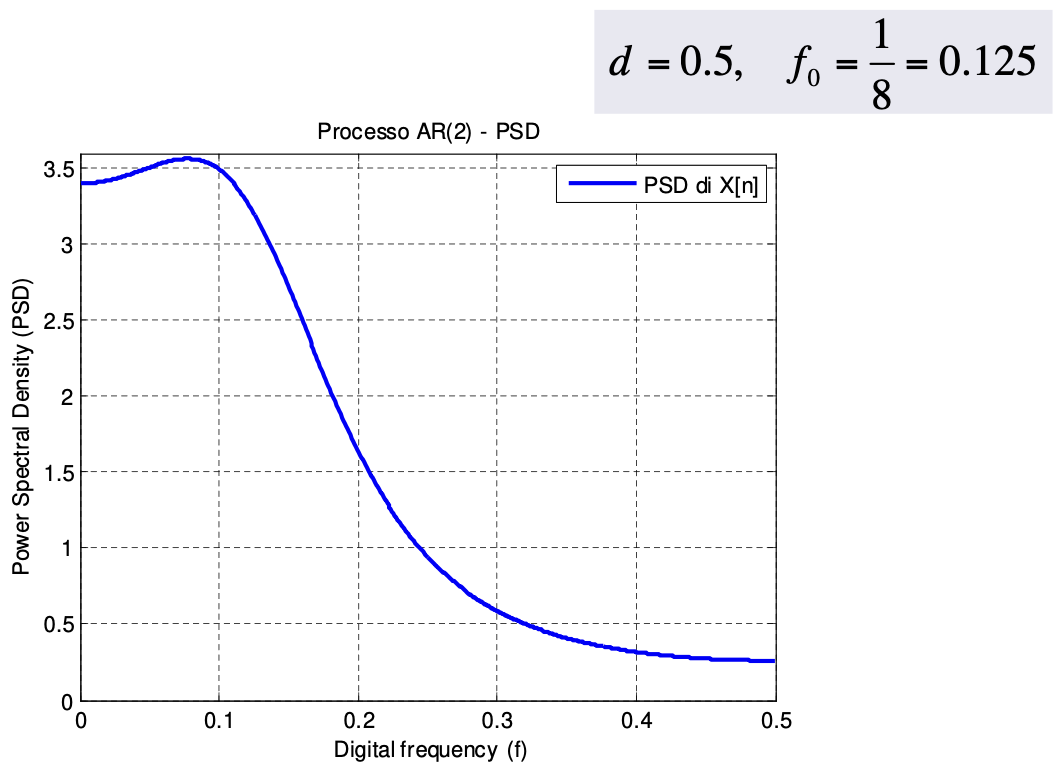
\includegraphics[width=0.65\linewidth]{Image/pdf 6/21.AR(2)_3.png}
    \label{fig:placeholder}
\end{figure}
\begin{figure}[H]
    \centering
    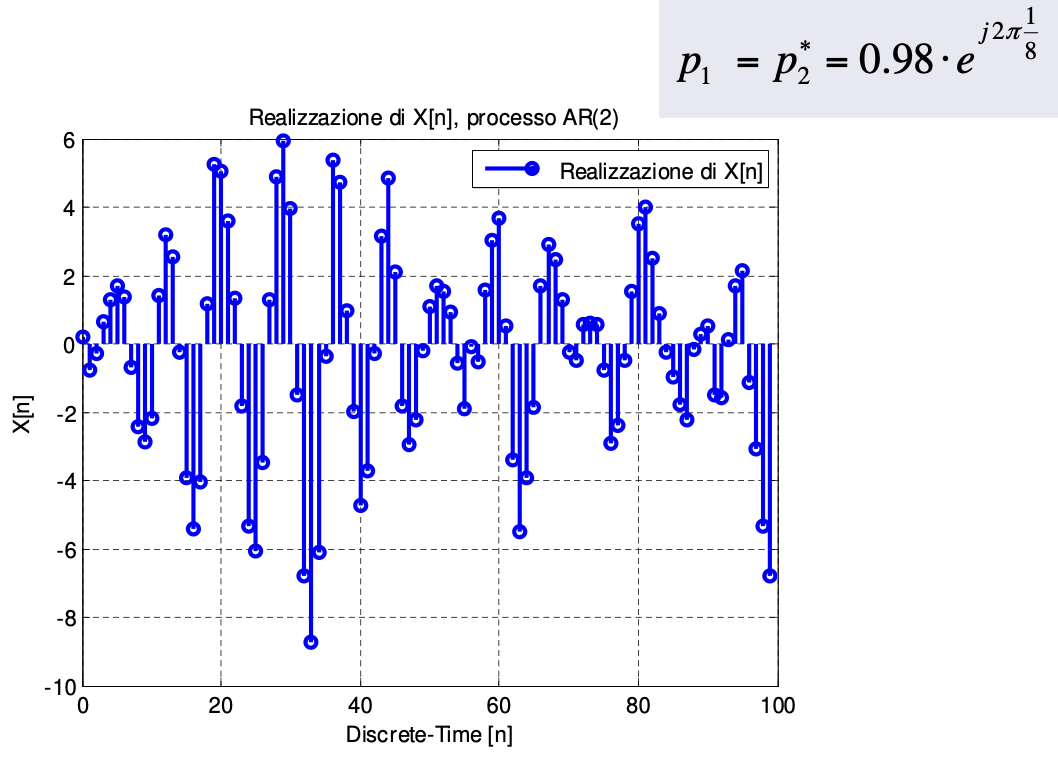
\includegraphics[width=0.65\linewidth]{Image/pdf 6/22.AR(2)_4.png}
    \label{fig:placeholder}
\end{figure}
\begin{figure}[H]
    \centering
    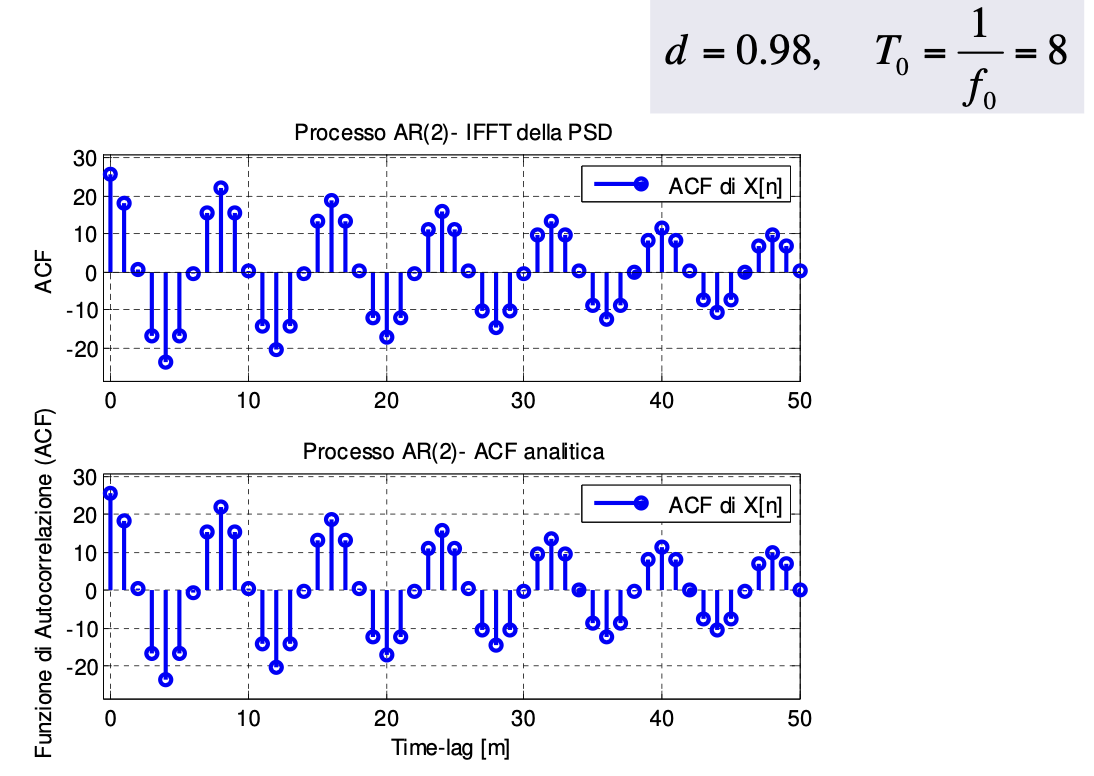
\includegraphics[width=0.65\linewidth]{Image/pdf 6/23.AR(2)_5.png}
    \label{fig:placeholder}
\end{figure}
\begin{figure}[H]
    \centering
    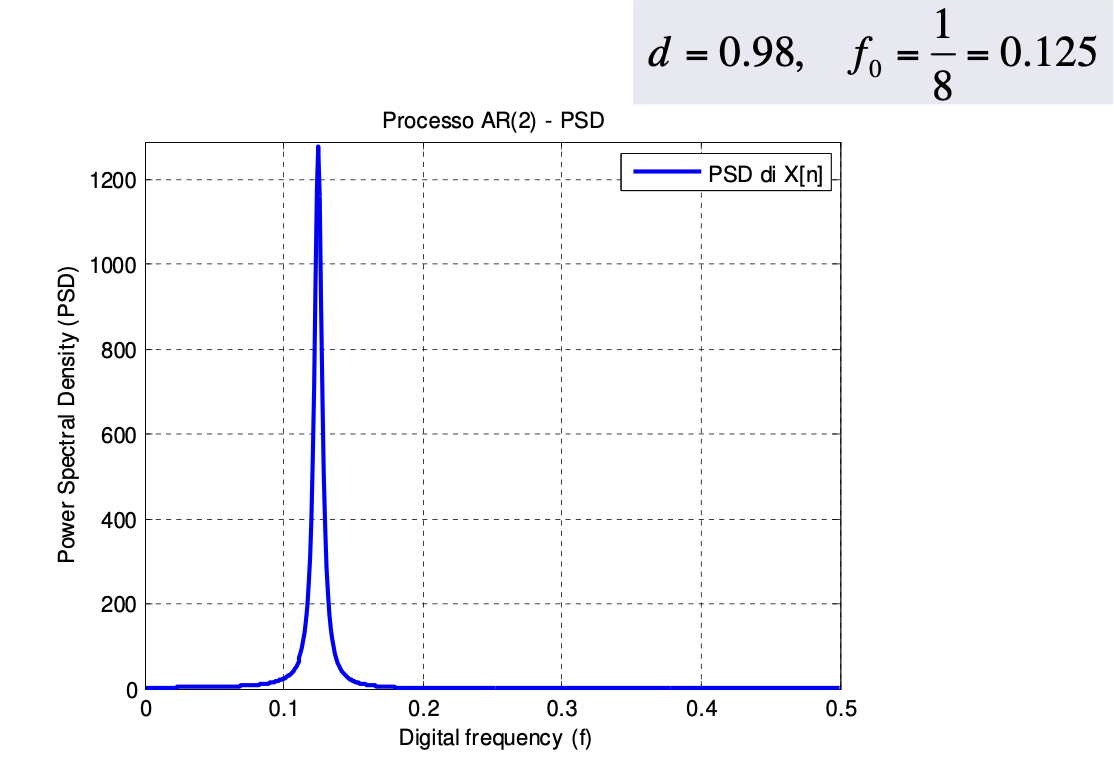
\includegraphics[width=0.65\linewidth]{Image/pdf 6/24.AR(2)_6.png}
    \label{fig:placeholder}
\end{figure}
\end{itemize}
\subsubsection{Moving average processes: MA(Q)}
\begin{figure}[H]
    \centering
    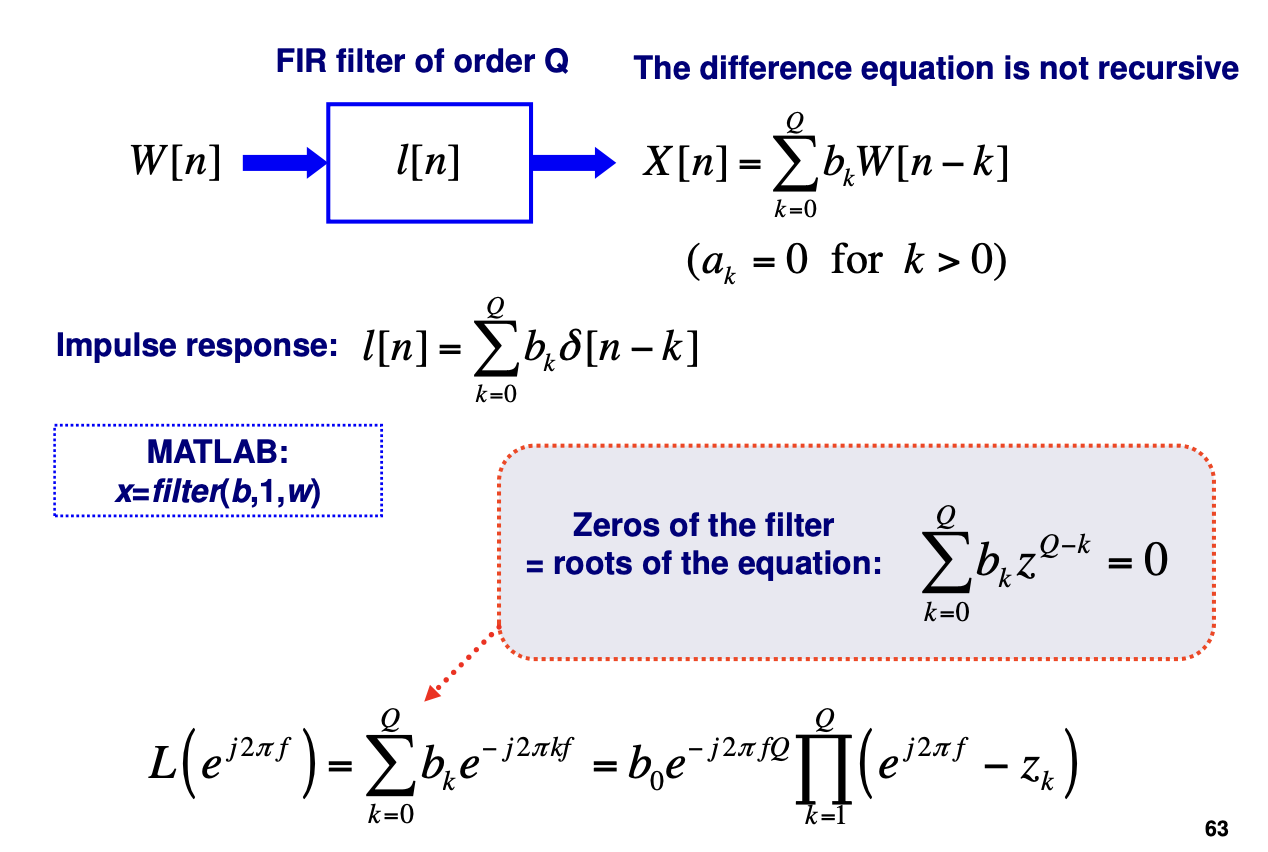
\includegraphics[width=0.65\linewidth]{Image/pdf 6/25.MA(Q).png}
    \label{fig:placeholder}
\end{figure}
\begin{itemize}
    \item \textbf{Important}: for an MA(Q) process the \textbf{correlation time} is equal to the length of the impulse response of the innovation filter, i.e. \(L_X=Q\).
\begin{align*}
    &l[n] = \sum_{k=0}^{Q} b_{k}\,\delta[n-k]
     = \begin{cases}
         b_{n}, & n = 0,1,\ldots,Q,\\[2pt]
         0,     & \text{otherwise}
       \end{cases}\\[4pt]
&R_{X}[m] = \sigma_{W}^{2}\, l[m] \otimes l[-m]\\[6pt]
&\text{If } l[n] \neq 0 \text{ for } 0 \le n \le Q \text{ then } R_{X}[m] \neq 0 \text{ for } |m| \le Q\\[4pt]
&\text{Frequency response: }L\!\left(e^{j2\pi f}\right) = \sum_{n=0}^{Q} b_{n} e^{-j2\pi f n}
\end{align*}
\begin{figure}[H]
    \centering
    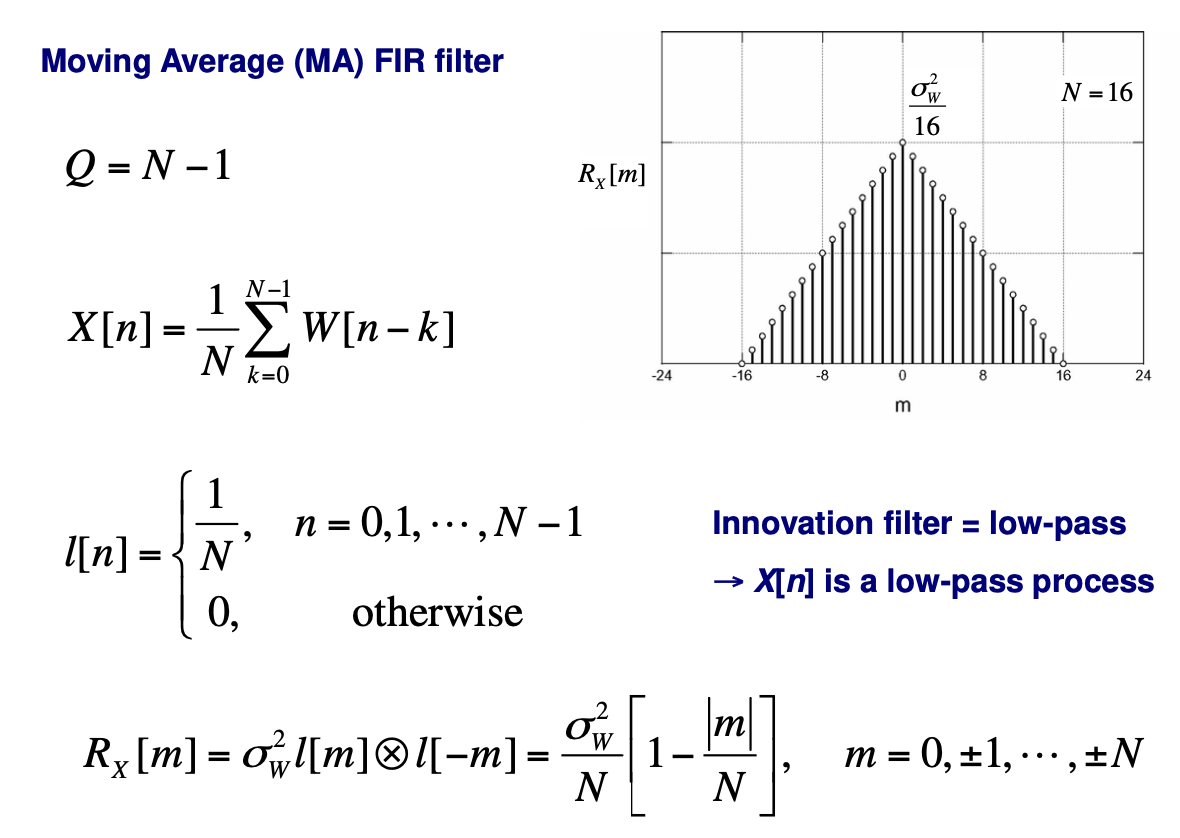
\includegraphics[width=0.65\linewidth]{Image/pdf 6/27.MA(Q)_2.png}
    \label{fig:placeholder}
\end{figure}
\begin{align*}
L\!\left(e^{j2\pi f}\right)
  &= \sum_{n=0}^{N-1} \frac{1}{N} e^{-j2\pi f n}
  = \frac{1}{N} \sum_{n=0}^{N-1} \left(e^{-j2\pi f}\right)^{n}\\[4pt]
&= \frac{1}{N} \cdot \frac{1 - e^{-j2\pi f N}}{1 - e^{-j2\pi f}}
= \frac{1}{N} \cdot
  \frac{e^{j\pi f N} - e^{-j\pi f N}}{e^{j\pi f} - e^{-j\pi f}}
  \, e^{-j\pi f (N-1)}\\[4pt]
&= \frac{1}{N} \cdot
  \frac{e^{j\pi f N} - e^{-j\pi f N}}{2j} \cdot
  \frac{2j}{e^{j\pi f} - e^{-j\pi f}}\,
  e^{-j\pi f (N-1)}\\[4pt]
&= \frac{1}{N} \cdot
  \frac{\sin(\pi f N)}{\sin(\pi f)}\,
  e^{-j\pi f (N-1)}
= \frac{\pi f}{N\pi f}\,
  \frac{\sin(\pi f N)}{\sin(\pi f)}\,
  e^{-j\pi f (N-1)}
\end{align*}
\item This is equal to a \textbf{"discrete sinc"}:
\[
L(e^{j2\pi f})=\frac{\text{sinc}(Nf)}{\text{sinc}(f)}e^{-j\pi f(N-1)}
\]
\begin{figure}[H]
    \centering
    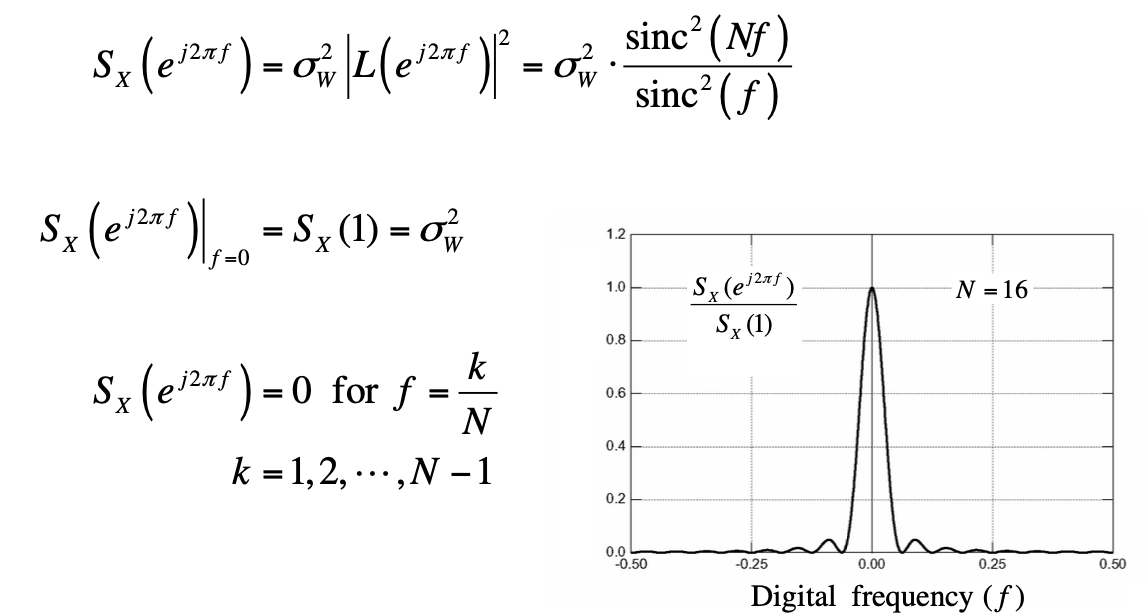
\includegraphics[width=0.65\linewidth]{Image/pdf 6/28.MA(Q)_bo.png}
    \label{fig:placeholder}
\end{figure}
\item \textbf{Model identification problem}: given the observation of \(N\) samples of the process \(X[n]\), \(n=0,1,2,\cdots,N-1\), we want to find the best model to represent this process.
\item Identify the ARMA(P,Q) model means to find the parameters of the model that best represnets these data:
\[
\{\sigma_W^2,\textbf{a},\textbf{b}\}\quad\Rightarrow\quad P+Q+1\text{ unknown parameters}
\]
\item Actually, the orders \(P\) and \(Q\) of the AR and MA are also generally unknown. The problem of estimating \(P\) and \(Q\) from  the data is called \textbf{Model Order Selection (MOS)}. We do not care.
\item In order to solve the model identification problem we apply the \textbf{Method of Moments}(Maximum Likelihood estimate is also possible, but the solution is much more difficult to find and it is not in closed form).
\item The first step is to find a relationship between the unknown parameters and some moments of the process. We use to this purpose the ACF, that in the case of real-valued processes is defined as:
\begin{align*}
\text{ACF:}\qquad
R_{X}[m] &= E\{X[n]X[n+m]\} \\[4pt]
R_{X}[m] &= R_{X}[-m] = E\{X[n]X[n-m]\}
\end{align*}

\item To find the relationship that we need, let us multiply all the terms of the ARMA recursive equation by \(X[n-m]\), assuming that \(m\geq0\):
\begin{align*}
&X[n] = \sum_{k=1}^{P} a_{k} X[n-k] + \sum_{k=0}^{Q} b_{k} W[n-k] \\[6pt]
&X[n]X[n-m] = \sum_{k=1}^{P} a_{k} X[n-k] X[n-m]
          + \sum_{k=0}^{Q} b_{k} W[n-k] X[n-m]
\end{align*}
\item Then, we calculate the statistical expectation of all terms:
\begin{align*}
E\{X[n]X[n-m]\}
&= \sum_{k=1}^{P} a_{k}\,E\{X[n-k]X[n-m]\}
 + \sum_{k=0}^{Q} b_{k}\,E\{W[n-k]X[n-m]\} \\[6pt]
R_{X}[m]
&= \sum_{k=1}^{P} a_{k}\,R_{X}[m-k]
 + \sum_{k=0}^{Q} b_{k}\,R_{XW}[m-k]
\end{align*}

\item The cross-correlation function between the innovation process \(W[n]\) (input of the innovation filter) and the process \(X[n]\)(output of the innovation filter) is defined as follows and it is not a symmetric function:
\begin{align*}
R_{XW}[m]
&\triangleq E\{X[n]W[n+m]\}
 = E\{X[n-m]W[n]\}
 = E\{W[n]X[n-m]\} \\[4pt]
&= R_{WX}[-m] \ne R_{XW}[-m]
 = E\{X[n]W[n-m]\}
\end{align*}

\item To derive this cross-correlation function, remeber that \(X[n]\) is the output of a causal filter, the innovation filter, whose impulse response \(l[n]\) is causal, when the input is the white process \(W[n]\) (it is a sequence of uncorrelated random variables):
\[
X[n]=l[n]*W[n]=\sum_{k=0}^{+\infty}l[k]W[n-k]
\]
\vspace{-0.5em}
\begin{align*}
R_{XW}[m]
&= E\{X[n]W[n+m]\}
 = \sum_{k=0}^{+\infty} l[k]\,
    E\{W[n-k]W[n+m]\} \\[4pt]
&= \sum_{k=0}^{+\infty} l[k]\,
    R_{W}[m+k]
 = \sigma_{W}^{2} \sum_{k=0}^{+\infty} l[k]\,
    \delta[m+k]
 = \sigma_{W}^{2} l[-m]
\end{align*}

\item Since \(l[n]\) is the impulse response of a causal filter, it is a causal signal, i.e. \(l[n]=0\) for \(n<0\). Hence, we have :
\begin{align*}
R_{XW}[m]
&=
\begin{cases}
0,            & m > 0,\\[2pt]
\sigma_{W}^{2} l[-m], & m \le 0
\end{cases}
\\[10pt]
\sum_{k=0}^{Q} b_{k} R_{XW}[m-k]
&= \sigma_{W}^{2} \sum_{k=0}^{Q} b_{k} l[k-m]
=
\begin{cases}
0, & m > Q,\\[4pt]
\sigma_{W}^{2} \displaystyle\sum_{k=m}^{Q} b_{k} l[k-m], & 0 \le m \le Q
\end{cases}
\end{align*}
\begin{align*}
\sum_{k=0}^{Q} b_{k} R_{XW}[m-k]
&=
\begin{cases}
0, & m > Q,\\[4pt]
\sigma_{W}^{2} \displaystyle\sum_{k=m}^{Q} b_{k} l[k-m], & 0 \le m \le Q
\end{cases}
\\[10pt]
\text{if we define } i \triangleq k-m \text{ we get} \qquad
\sum_{k=0}^{Q} b_{k} R_{XW}[m-k]
&=
\begin{cases}
0, & m > Q,\\[4pt]
\sigma_{W}^{2} \displaystyle\sum_{i=0}^{Q-m} l[i]\, b_{i+m}, & 0 \le m \le Q
\end{cases}
\end{align*}
\[\hspace{-2em}\boxed{R_X[m] = \sum_{k=1}^{P} a_k R_X[m-k] + \sum_{k=0}^{Q} b_k R_{XW}[m-k]
=
\begin{cases}
\displaystyle\sum_{k=1}^{P} a_k R_X[m-k], & m>Q \\[10pt]
\displaystyle\sum_{k=1}^{P} a_k R_X[m-k] 
        + \sigma_w^2 \sum_{k=0}^{Q-m} l[k]\,b_{k+m}, & 0\le m\le Q
\end{cases}}\]
\item For \(m<0\) we can exploit the simmetry of the ACF:
\[
R_X[m]=R_X[-m]
\]
\item If we set \(m=Q+1,Q+2,\cdots,Q+P\) we obtain \(P\) linear equations in the \(P\) unknowns:

\begin{align*}
&R_X[m] = \sum_{k=1}^{P} a_k R_X[m-k] \qquad \text{for } m = Q+1, Q+2, \dots, Q+P \\[10pt]
&\begin{bmatrix}
R_X[Q]      & R_X[Q-1]      & \cdots & R_X[Q-(P-1)] \\
R_X[Q+1]    & R_X[Q]        & \cdots & R_X[Q-(P-2)] \\
\vdots      & \vdots        & \ddots & \vdots       \\
R_X[Q+(P-1)]& R_X[Q+(P-2)]  & \cdots & R_X[Q]
\end{bmatrix}
\begin{bmatrix}
a_1 \\ a_2 \\ \vdots \\ a_P
\end{bmatrix}
=
\begin{bmatrix}
R_X[Q+1] \\ R_X[Q+2] \\ \vdots \\ R_X[Q+P]
\end{bmatrix}
\\[10pt]
&\mathbf{R}\,\mathbf{a} = \mathbf{r}
\;\;\Rightarrow\;\;
\mathbf{a} = \mathbf{R}^{-1}\mathbf{r}
\end{align*}

\item If we replace \textbf{R} and \textbf{r} with their estimates obtained by using the unbiased Sample Autocorrelation Function, we get an estimate of the AR coefficients:
\[
\mathbf{\hat{a}=\hat{R}^{-1}\hat{r}}
\]
\item \textbf{Important:} By inserting the estimate of vector \textbf{a} in the previous equations for \(m=0,1,2,\cdots,Q\) we get \(Q+1\) (nonlinear) equation in the \(Q+1\) unknowns:
\[
R_X[m]=\sum_{k=1}^{P}\hat{a}R_X[m-k]+\sigma^2_W\sum_{k=0}^{Q-m}l[k;\mathbf{\hat{a},b}],\quad 0\leq m\leq Q
\]
\item Since the above equations are non linear with respect to vector \textbf{b}, to estimate the MA coefficients is more computationally demanding than to estimate the AR coefficients.
\item For \textbf{MA(Q) processes} \(P=0\) and we have that \(l[k]=b_k\), hence we get:

\item This result tell us that: (1) the length of the ACF of an MA(Q) process is Q;(2) for MA(Q) procesesses the relationship between the ACF values and the unknown parameters \(\{b_k\}\) is \textbf{non-linear}, hence it is much more difficult to find the \(\{b_k\}\) coefficients than the \(\{a_k\}\) coefficients, given the ACF values.
\begin{align*}
R_X[m] = \sum_{k=0}^{Q} b_k R_{XW}[m-k]
&=
\begin{cases}
0, & m>Q \\[8pt]
\sigma_w^2 \displaystyle\sum_{k=0}^{Q-m} l[k]\,b_{k+m}, & 0\le m \le Q
\end{cases}\\[4pt]
&=
\begin{cases}
0, & m>Q \\[8pt]
\sigma_w^2 \displaystyle\sum_{k=0}^{Q-m} b_k b_{k+m}, & 0\le m \le Q
\end{cases}
\end{align*}

\end{itemize}
\subsubsection{The Yule-Walker (YW) equation for AR(P) processes}
\begin{itemize}
    \item For \textbf{AR(P) processes} \(Q=0\), taking into account that \(l[0]=1\) and \(b_0=1\),we get:
\begin{align*}
R_X[m] =
\begin{cases}
\displaystyle\sum_{k=1}^{P} a_k R_X[m-k], & m>0 \\[8pt]
\displaystyle\sum_{k=1}^{P} a_k R_X[m-k] + \sigma_w^2, & m=0
\end{cases}\\[4pt]
\qquad\Longrightarrow\qquad
R_X[m] = \sum_{k=1}^{P} a_k R_X[m-k] + \sigma_w^2 \delta[m], \quad m\ge 0
\end{align*}
\item \textbf{Important}: For an \textbf{AR(P)} process there is a \textbf{linear} relationship between the ACF values and the unknown parameters (in this case: the power of the innovation process and the \(\{a_k\}\) coefficients). The euqations above are called \textbf{Yule-Walker (YW) equations} and can be expressed in matrix form by calculating it for \(m=0,1,2,\cdots,P\), being \(P+1\) the number of unknowns.
\[
R_X[m]-\sum_{k=1}^{P}a_kR_X[m-k]=\sigma_W^2\delta[m],\quad m\geq 0
\]
\item Since we have \(P+1\) unknowns, we need (at least) \(P+1\) equations, so we calculate the YW equation for \(m=0,1,2,\cdots,P\):

\begin{align*}
m=0:\;& R_X[0] - a_1 R_X[-1] - a_2 R_X[-2] - \cdots - a_P R_X[-P] = \sigma_w^2 \\[4pt]
m=1:\;& R_X[1] - a_1 R_X[0]  - a_2 R_X[-1] - \cdots - a_P R_X[-P+1] = 0 \\[4pt]
m=2:\;& R_X[2] - a_1 R_X[1]  - a_2 R_X[0]  - \cdots - a_P R_X[-P+2] = 0 \\[4pt]
&\vdots \\[4pt]
m=P:\;& R_X[P] - a_1 R_X[P-1] - a_2 R_X[P-2] - \cdots - a_P R_X[0] = 0
\end{align*}

\item This system of \(P+1\) linear equations can be expressed in matrix form.

\[
\begin{bmatrix}
R_X[0]   & R_X[-1] & R_X[-2] & \cdots & R_X[-P] \\
R_X[1]   & R_X[0]  & R_X[-1] & \cdots & R_X[-(P-1)] \\
R_X[2]   & R_X[1]  & R_X[0]  & \cdots & R_X[-(P-2)] \\
\vdots   & \vdots  & \vdots  & \ddots & \vdots     \\
R_X[P]   & R_X[P-1]& R_X[P-2]& \cdots & R_X[0]
\end{bmatrix}
\begin{bmatrix}
1 \\ -a_1 \\ -a_2 \\ \vdots \\ -a_P
\end{bmatrix}
=
\begin{bmatrix}
\sigma_w^2 \\ 0 \\ 0 \\ \vdots \\ 0
\end{bmatrix}
\]
\item The \textbf{Yule-Walker} equations can be expressed in a more compact form as follows:
\[
\mathbf{C}_X \triangleq
\begin{bmatrix}
R_X[0]   & R_X[-1]   & \cdots & R_X[-(P-1)] \\
R_X[1]   & R_X[0]    & \cdots & R_X[-(P-2)] \\
\vdots   & \vdots    & \ddots & \vdots      \\
R_X[P-1] & R_X[P-2]  & \cdots & R_X[0]
\end{bmatrix},
\qquad
\mathbf{c}_X \triangleq
\begin{bmatrix}
R_X[1] \\ R_X[2] \\ \vdots \\ R_X[P]
\end{bmatrix},
\qquad
\mathbf{a} \triangleq
\begin{bmatrix}
a_1 \\ a_2 \\ \vdots \\ a_P
\end{bmatrix}
\]
\[
\begin{bmatrix}
R_X[0] & \mathbf{c}_X^{T} \\
\mathbf{c}_X & \mathbf{C}_X
\end{bmatrix}
\begin{bmatrix}
1 \\ -\mathbf{a}
\end{bmatrix}
=
\begin{bmatrix}
\sigma_w^2 \\ 0
\end{bmatrix}
\;\;\Longrightarrow\;\;
\begin{cases}
R_X[0] - \mathbf{c}_X^{T}\mathbf{a} = \sigma_w^2 \\[4pt]
\mathbf{c}_X - \mathbf{C}_X \mathbf{a} = 0
\end{cases}
\]
\item The second matrix equation can be easily solved w.r.t \textbf{a} if the covariance matrix \(\mathbf{C_x}\) is full rank (the covariance matrix of a regular process that satisfies the Paley-Wiener condition is always full-rank),and then the power of \(W[n]\) is immediately derived:
\[\boxed{\begin{cases}
\mathbf{a} = \mathbf{C}_X^{-1}\mathbf{c}_X \\[4pt]
\sigma_w^{2} = R_X[0] - \mathbf{c}_X^{T}\mathbf{C}_X^{-1}\mathbf{c}_X
\end{cases}}
\]
\item Covariance matrix \(\mathbf{C_X}\) is simmetric and it has the Toeplitz structure: these properties are exploited by the \textbf{Levinson-Durbin} and \textbf{Schur} algorithms to solve the linear system of \(P\) equations with complexity of the order \(P^2\) instead of \(P^3\).
\end{itemize}
\subsubsection{Model identification by using AR(P) models}
\begin{itemize}
\item To identify an \textbf{AR(P) model},i.e. derive the \(\{a_k\}\) coefficients and the innovation process power, we have to solve a \textbf{linear} system of equations of order \(P+1\).
\item To identify a \textbf{MA(Q) model}, i.e. derive the \(\{b_k\}\) coefficients and the power of the innovation process, we have to solve a \textbf{non-linear} system of equations of order \(Q+1\); this is true also for an ARMA model. For this reason, \underline{AR models are much more frequently used than MA or ARMA models}.
\item \underline{\textbf{Identification of an AR(P) model}}:
\noindent \textbf{Step 1}: estimate the ACF values for \(m=0,1,2,\cdots,P\) via the \textbf{samples estimates}:
\[
\{X[n]\}_{n=0}^{N-1}\quad\Rightarrow\quad\hat{R}_X[m] = \frac{1}{N-m}\sum_{n=0}^{N-m-1} X[n]\,X[n+m], \qquad m = 0,1,2,\dots,P
\]
\item Where typically \(P\ll N\), so we can use the unbiased sample estimator.
\begin{align*}
E\{\hat{R}_X[m]\}
&= \frac{1}{N-m}\sum_{n=0}^{N-m-1} E\{X[n]X[n+m]\}\\[4pt]
&= \frac{1}{N-m}\sum_{n=0}^{N-m-1} R_X[m]
= R_X[m], \quad m = 0,1,2,\dots,P
\end{align*}

\item So the estimates are unbiased:
\[
MSE\{\hat{R}_X[m]\}\approx \frac{\text{var}\{X[n]X[n+m]\}}{N-m},\quad m=0,1,2,\cdots ,P
\]
\item The \textbf{Sample Autocorrelation }estimator is \textbf{consistent}, i.e. th estimates of the ACF values for \(m=0,1,2,\cdots,P\), converge in probability and mean square sense to the true values when \(N\rightarrow \infty\).
\begin{align*}
&\hat{R}_X[m] = \frac{1}{N-m}\sum_{n=0}^{N-m-1} X[n]X[n+m], \quad m = 0,1,2,\dots,P \\[10pt]
&\hat{\mathbf{C}}_X \triangleq
\begin{bmatrix}
\hat{R}_X[0]   & \hat{R}_X[-1]   & \cdots & \hat{R}_X[-(P-1)] \\
\hat{R}_X[1]   & \hat{R}_X[0]    & \cdots & \hat{R}_X[-(P-2)] \\
\vdots         & \vdots          & \ddots & \vdots            \\
\hat{R}_X[P-1] & \hat{R}_X[P-2]  & \cdots & \hat{R}_X[0]
\end{bmatrix},
\qquad
\hat{\mathbf{c}}_X \triangleq
\begin{bmatrix}
\hat{R}_X[1] \\ \hat{R}_X[2] \\ \vdots \\ \hat{R}_X[P]
\end{bmatrix}
\end{align*}
\item \textbf{Step 2}: by applying the \textbf{Levinson-Durbin algortihm} or \textbf{Schur algorithm}, solve the \textbf{Yule-Walker} linear system of equations and find the AR(P) model that better fits the estimated ACF sequence, i.e. the AR(P) model whose first P+1 values of the ACF are equal to the estimated ones:
\[{\begin{cases}
\mathbf{a} = \mathbf{C}_X^{-1}\mathbf{c}_X \\[4pt]
\sigma_w^{2} = R_X[0] - \mathbf{c}_X^{T}\mathbf{C}_X^{-1}\mathbf{c}_X
\end{cases}}
\]
\item \textbf{Step 3}: Once the AR(P) model parameters have been estimated, a (\underline{parametric}) estimate of the \textbf{PSD} can be immediately obtained as follows:
\[\hat{S}_X\!\left(e^{j2\pi f}\right)
= \hat{\sigma}_W^{\,2}\left|\hat{L}\!\left(e^{j2\pi f}\right)\right|^{2}
= \frac{\hat{\sigma}_W^{\,2}}{\left|\,1-\displaystyle\sum_{k=1}^{P}\hat{a}_k e^{-j2\pi k f}\right|^{2}}
\]
\item The estimates of the ACF for \(m<P\) can be derived from the recursive equation that we obtain for AR(P) processes:
\[
R_X[m]=\sum_{k=1}^{P}a_kR_X[m-k],\quad m>p
\]
\item By making use of the estimates of the ACF from \(m=0\) to \(m=P\), previously obtained by using the sample autocorrelation estimator, we can recursively an estimate of the ACF values for \(m=P+1,\) \(P+2\), \(P+3,\) \(\cdots,\) as follows:
\[
\hat{R}_X[m]=\sum_{k=1}^{P}\hat{a}_k\hat{R}_X[m-k],\quad m=P+1,P+2,\cdots
\]
\item The problem of \underline{\textbf{model identification}} by using an \textbf{AR(P)} model consists in the estimation of the unknown parameters \textbf{a} and the power of the AR(P) model whose first \(P+1\) values obtained by the sample estimator, by processing N samples of \(X[n]\):
\[
\{X[n]\}_{n=0}^{N-1}
\;\Rightarrow\;
\{\hat{R}_X[m]\}_{m=0}^{P}
\;\Rightarrow\;
\{\hat{\sigma}_w^{2}, \hat{\mathbf{a}}\}
\;\Rightarrow\;
\hat{S}_X\!\left(e^{j 2 \pi f}\right)
\]
\item \underline{Model identification by using an AR(P) model requires the solution of a system of \(P+1\) \textbf{linear}}\\
\noindent \underline{equations}; once we have an estimate of \textbf{a}, we derive an estimate of the power of the innovation process \(W[n]\).
\item Once the parameters of the AR(P) model we have been estimated, a (parametric) estimate of the PSD is obtained as:
\[
\hat{S}_X(e^{j2\pi f})=\frac{\hat{\sigma}_W^2}{\left|1-\sum_{k=1}^P\hat{a}_ke^{-j2\pi kf }\right|}
\]
\item \textbf{Example}: Let is consider the following \textbf{broadband ARMA(4,4) process} whose innovation filter has system function:
\begin{align*}
H(z) = \frac{B(z)}{A(z)}
&=
\frac{1 - 1.3817 z^{-1} + 1.5632 z^{-2} - 0.8843 z^{-3} + 0.4096 z^{-4}}
     {1 - 0.3544 z^{-1} + 0.3508 z^{-2} + 0.1736 z^{-3} + 0.2401 z^{-4}}
\end{align*}
\begin{align*}
&X[n]
= \underbrace{ 0.3544 \cdot X[n-1] - 0.3508 \cdot X[n-2] - 0.1736 \cdot X[n-3] - 0.2401 \cdot X[n-4]}_{\text{AR part}} \\[6pt]
&+\underbrace{ W[n] - 1.3817 \cdot W[n-1] + 1.5632 \cdot W[n-2] - 0.8843 \cdot W[n-3] + 0.4096 \cdot W[n-4]}_{\text{MA part}}
\end{align*}
\begin{figure}[H]
    \centering
    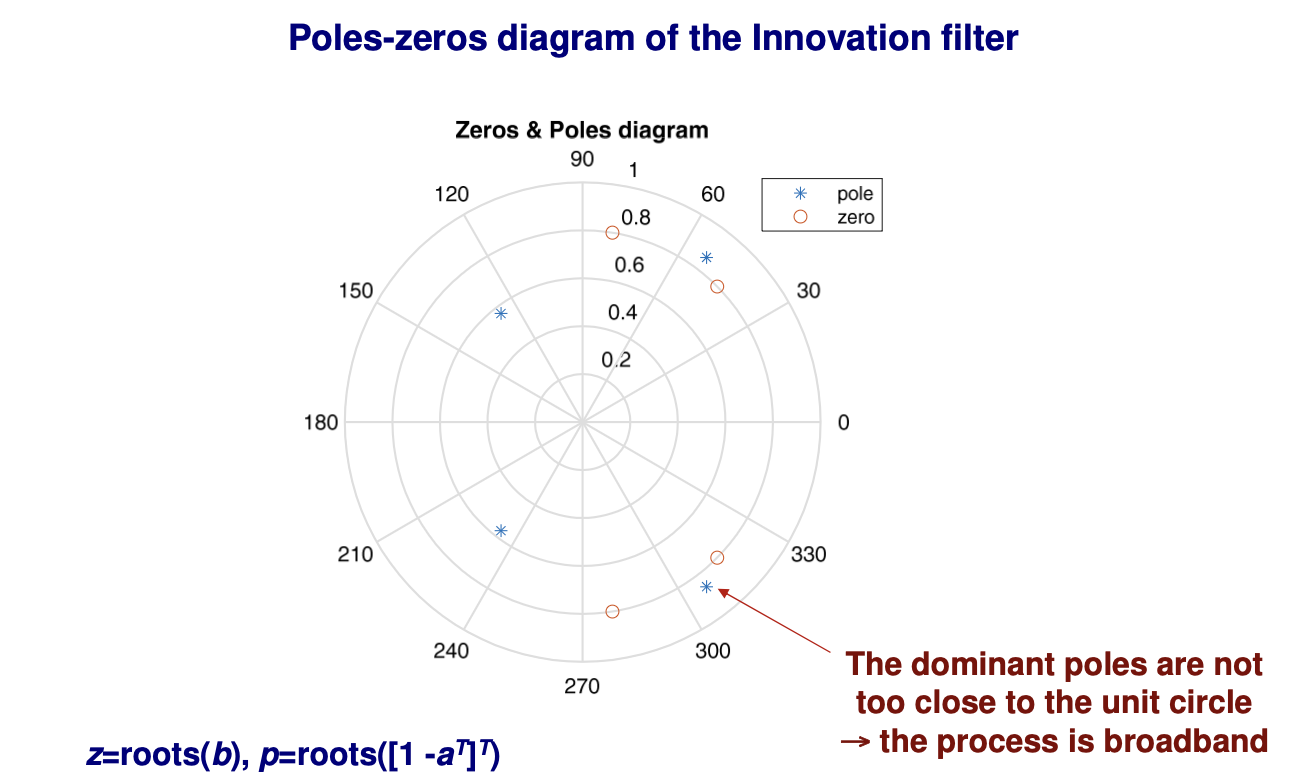
\includegraphics[width=0.65\linewidth]{Image/pdf 6/29.Zero_Pole.png}
    \label{fig:placeholder}
\end{figure}
\begin{figure}[H]
    \centering
    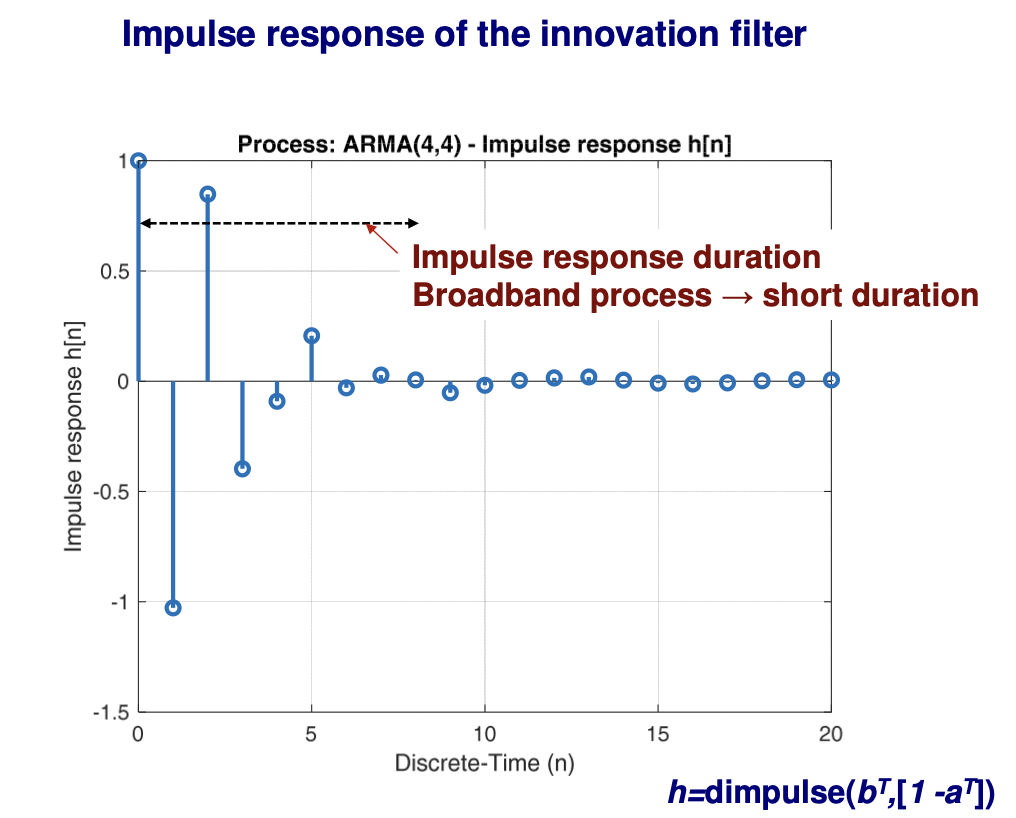
\includegraphics[width=0.65\linewidth]{Image/pdf 6/30.Impulse_resp.png}
    \label{fig:placeholder}
\end{figure}
\begin{figure}[H]
    \centering
    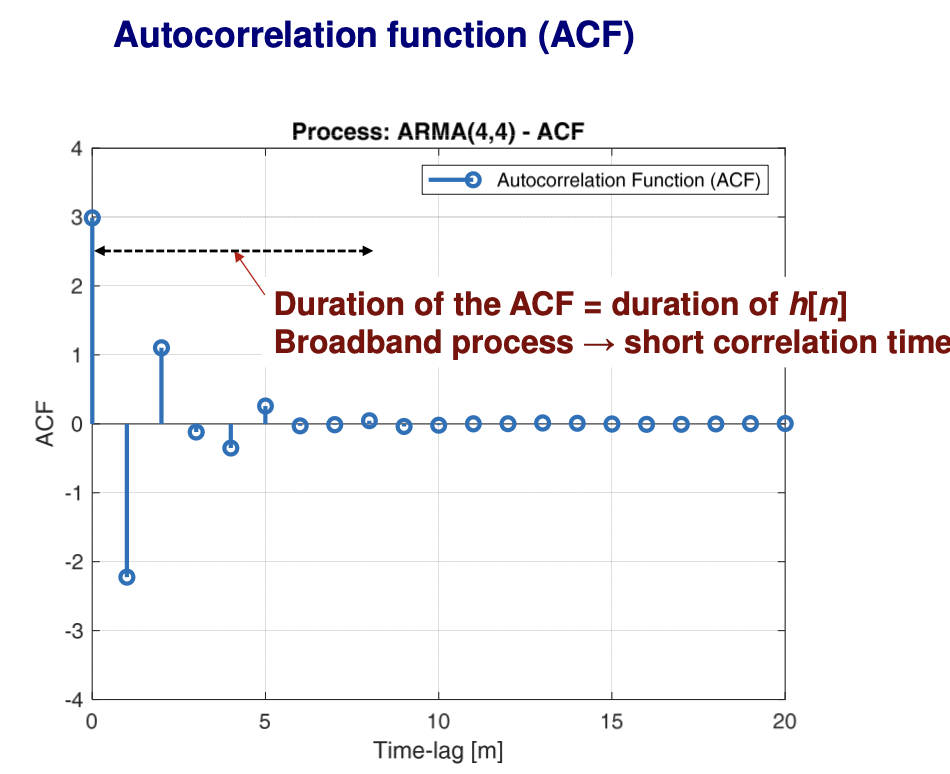
\includegraphics[width=0.65\linewidth]{Image/pdf 6/31.ACF.png}
    \label{fig:placeholder}
\end{figure}
\begin{figure}[H]
    \centering
    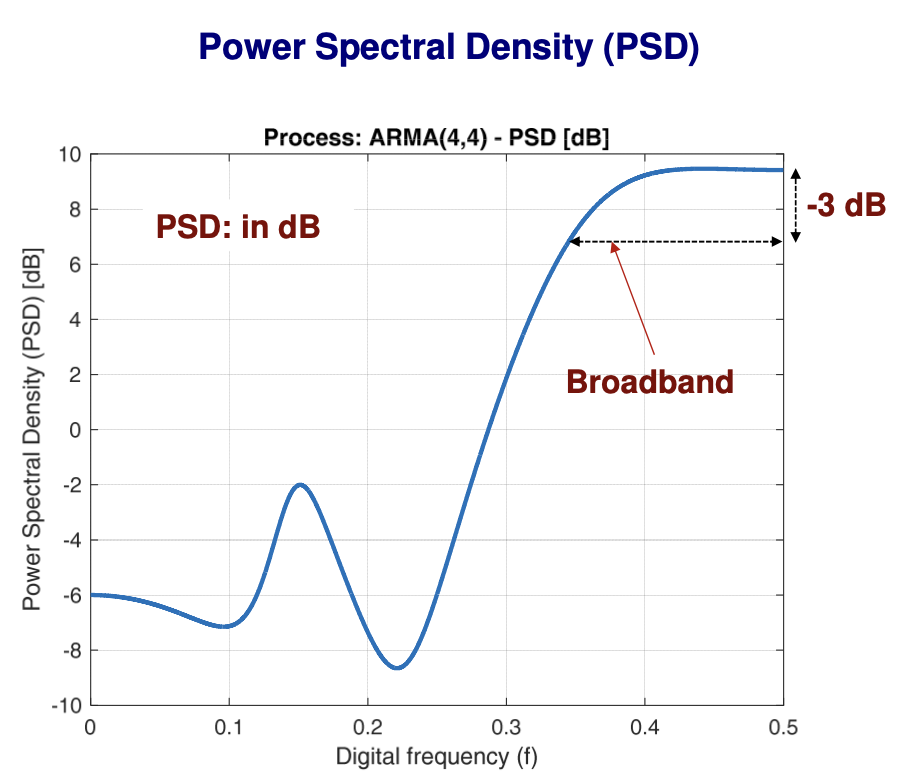
\includegraphics[width=0.65\linewidth]{Image/pdf 6/32.PSD.png}
    \label{fig:placeholder}
\end{figure}
\item \textbf{Definition of the PSD of a WSS discrete-time random process}:
\begin{align*}
S_X&\!\left(e^{j 2\pi f}\right)
= \lim_{N \to \infty} \frac{1}{N}
   E\!\left\{ \left| X_N\!\left(e^{j 2\pi f}\right) \right|^{2} \right\} = E\!\left\{ \lim_{N \to \infty} \frac{1}{N}
   \left| \sum_{n=0}^{N-1} x[n] e^{-j 2\pi f n} \right|^{2} \right\}\\[4pt]
&\text{where} \quad
X_N\!\left(e^{j 2\pi f}\right) \triangleq DTFT\{X[n]\}
= \sum_{n=0}^{N-1} x[n] e^{-j 2\pi f n}.
\end{align*}

\item The method of the \textbf{Periodigram}(Schuster's Periodogram) derives directly from this definition of the PSD and it is a \textbf{non-parametric non-adaptive method}:
\begin{align*}
\hat{S}_X^{(p)}\!\left(e^{j 2\pi \frac{k}{N}}\right)
&= \frac{1}{N}
   \left|
      \sum_{n=0}^{N-1} x[n] \,
      e^{-j 2\pi \frac{k}{N} n}
   \right|^{2},
   \qquad 0 \le k \le N-1
\end{align*}

\item \underline{\textbf{Periodogram}}: when N goes to infinity, for regular processes, we have:
\begin{align*}
\lim_{N \to \infty} E \left\{
   \hat{S}_X^{(p)}\!\left(e^{j 2\pi \frac{k}{N}}\right)
\right\}
&= S_X\!\left(e^{j 2\pi \tfrac{k}{N}}\right), \\[6pt]
\lim_{N \to \infty} \operatorname{var} \left\{
   \hat{S}_X^{(p)}\!\left(e^{j 2\pi \frac{k}{N}}\right)
\right\}
&= S_X^{2}\!\left(e^{j 2\pi \tfrac{k}{N}}\right).
\end{align*}

\item \underline{\textbf{In summary}}:
\begin{itemize}
    \item Regarding \textbf{Regualr processes}(continuous PSD) the \textbf{Periodogram} is an asymptotically unbiased but not consistent estimator, since its variance does not tend to zero as \(N\) goes to infinity.
    \item The variance of the estimate is asymptotically proportional to the square of the value of the PSD, then the MSE is greater where the PSD is greater.
    \item For \textbf{Predictable processes}(discrete PSD), the \textbf{Periodogram} is indeed an asymptotically unbiased and consistent estimator.
\end{itemize}
\begin{figure}[H]
    \centering
    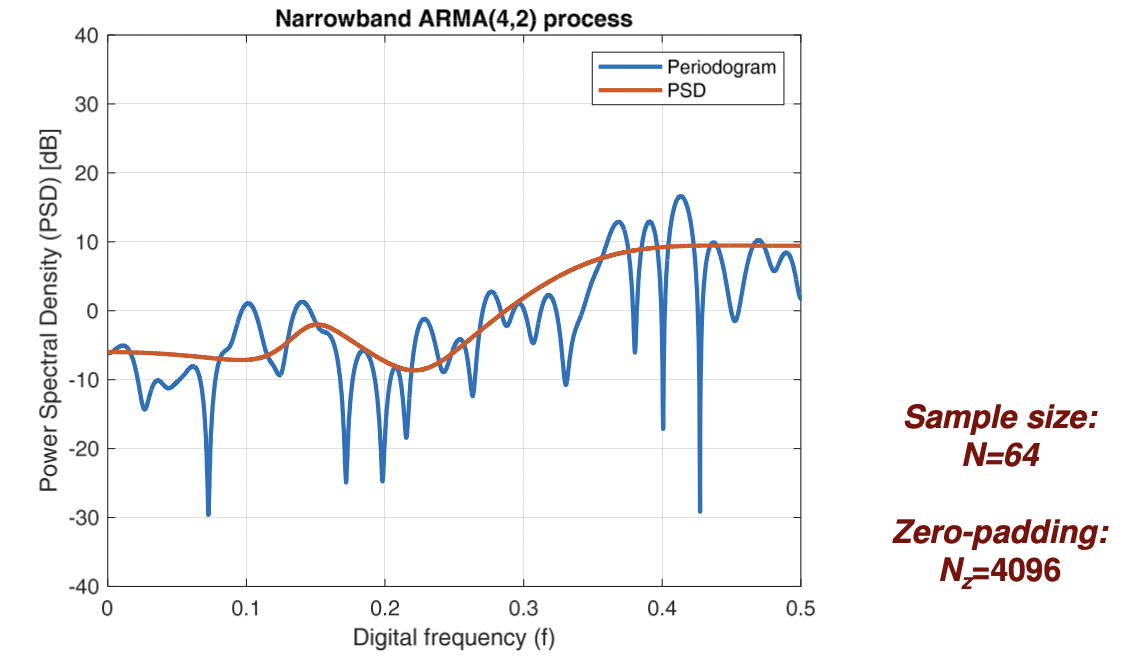
\includegraphics[width=0.65\linewidth]{Image/pdf 6/33.PSD_N64.png}
    \label{fig:placeholder}
\end{figure}
\begin{figure}[H]
    \centering
    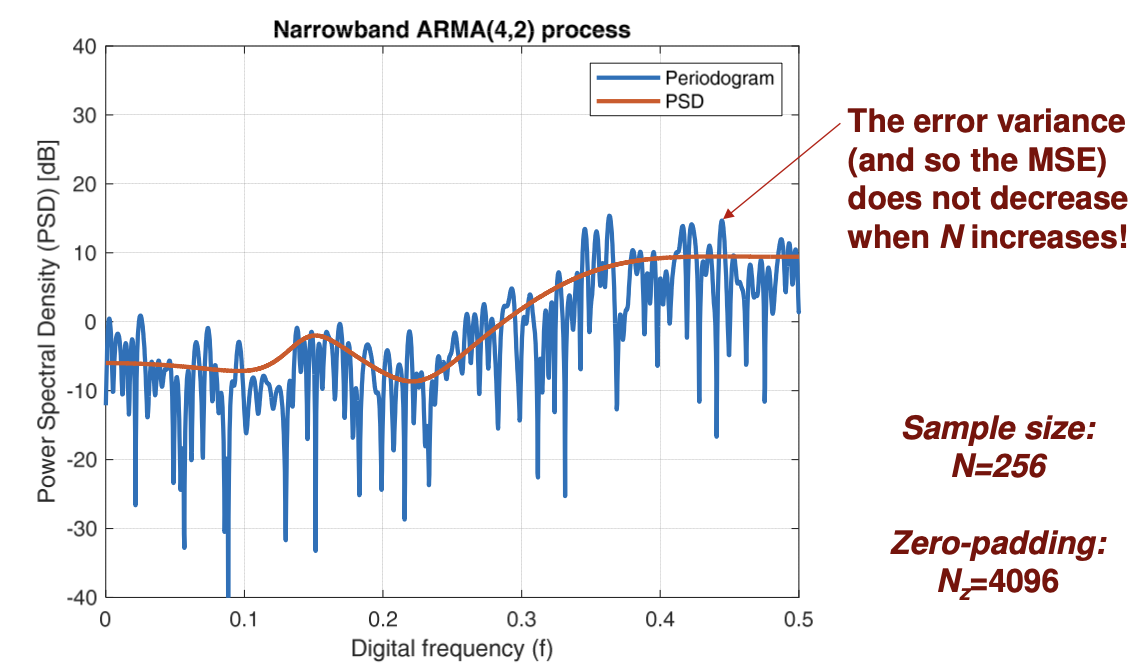
\includegraphics[width=0.65\linewidth]{Image/pdf 6/34.PSD_N256.png}
    \label{fig:placeholder}
\end{figure}
\begin{figure}[H]
    \centering
    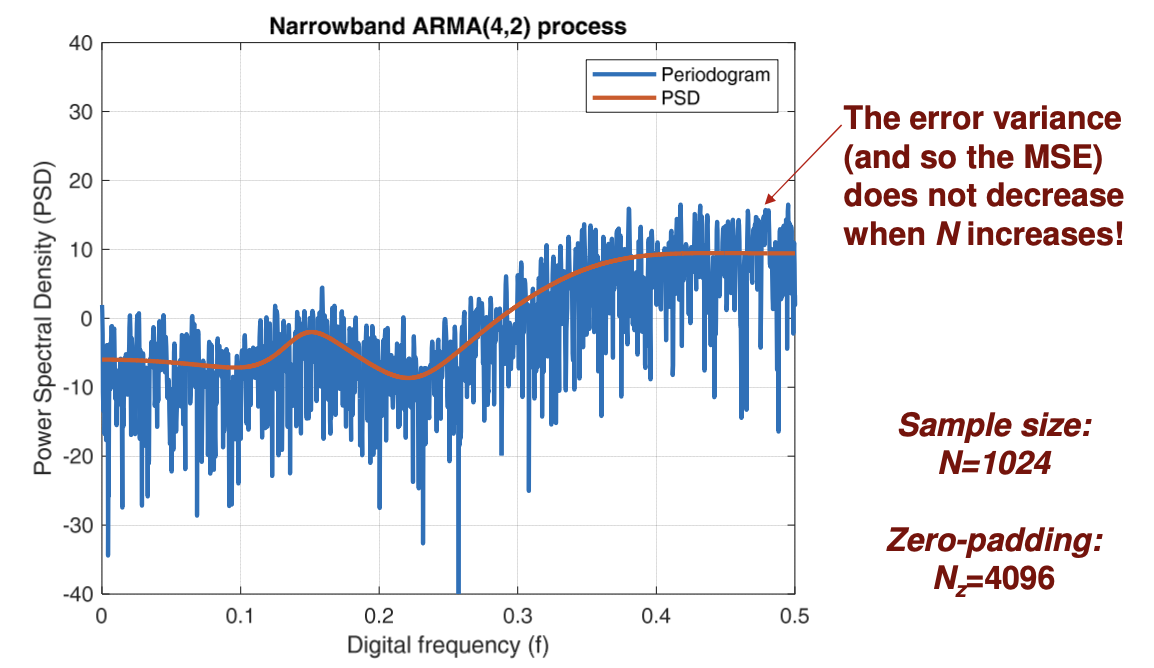
\includegraphics[width=0.65\linewidth]{Image/pdf 6/35.PSD_N1024.png}
    \label{fig:placeholder}
\end{figure}
\begin{figure}[H]
    \centering
    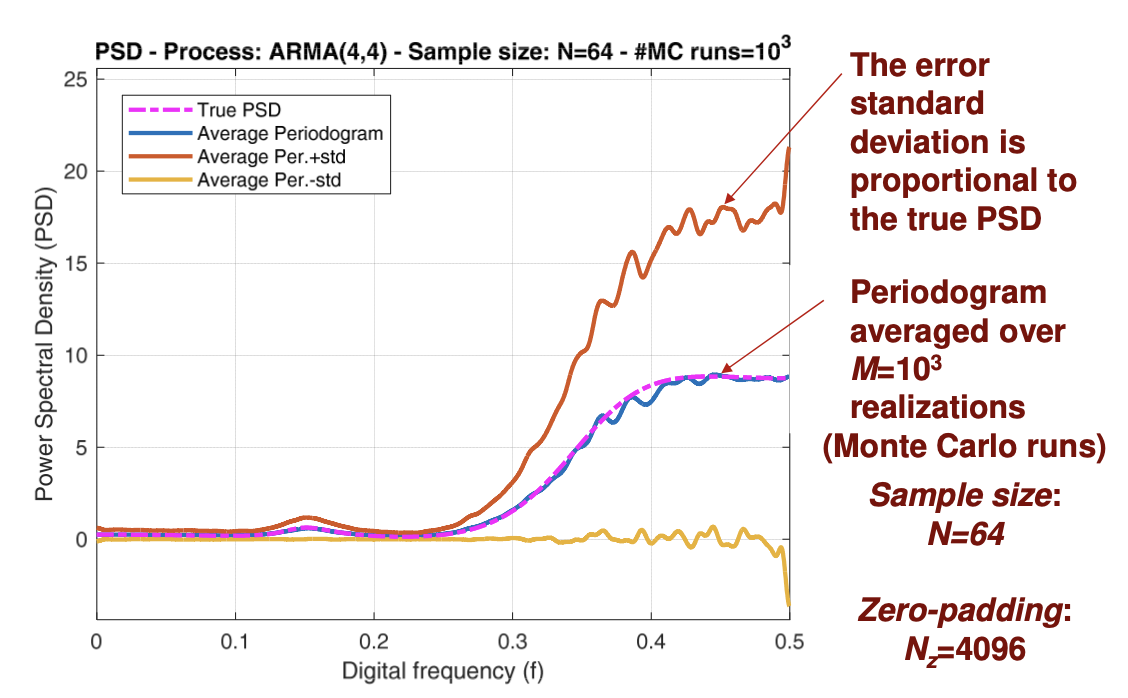
\includegraphics[width=0.65\linewidth]{Image/pdf 6/36.Periodo_N64.png}
    \label{fig:placeholder}
\end{figure}
\begin{figure}[H]
    \centering
    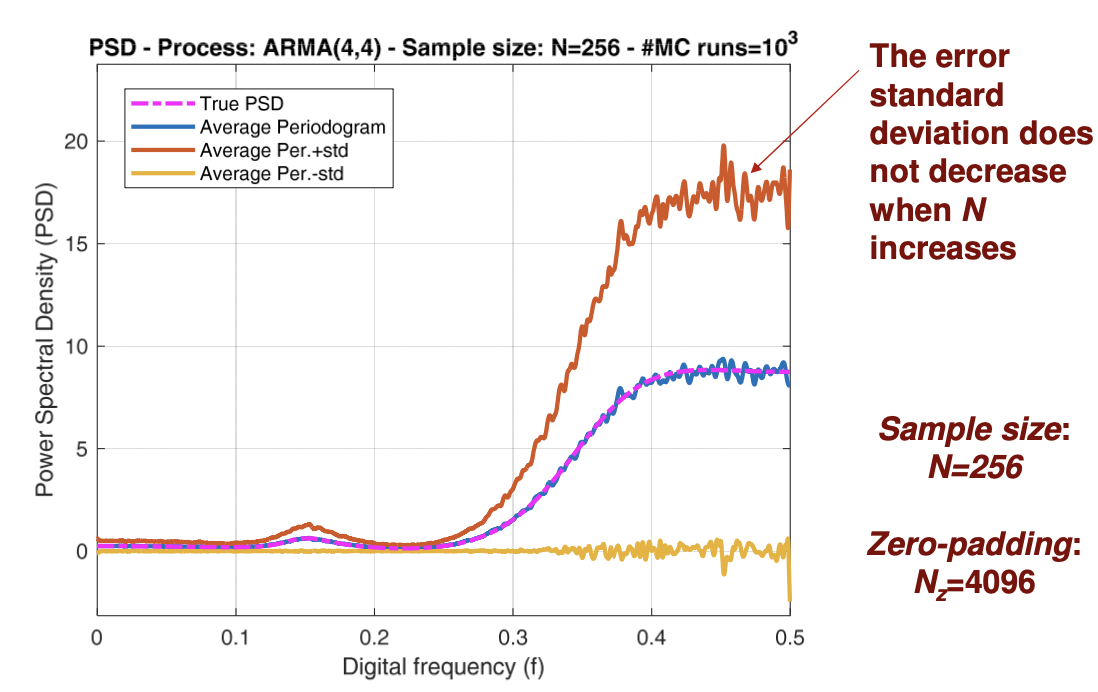
\includegraphics[width=0.65\linewidth]{Image/pdf 6/37.Periodo_N256.png}
    \label{fig:placeholder}
\end{figure}
\begin{figure}[H]
    \centering
    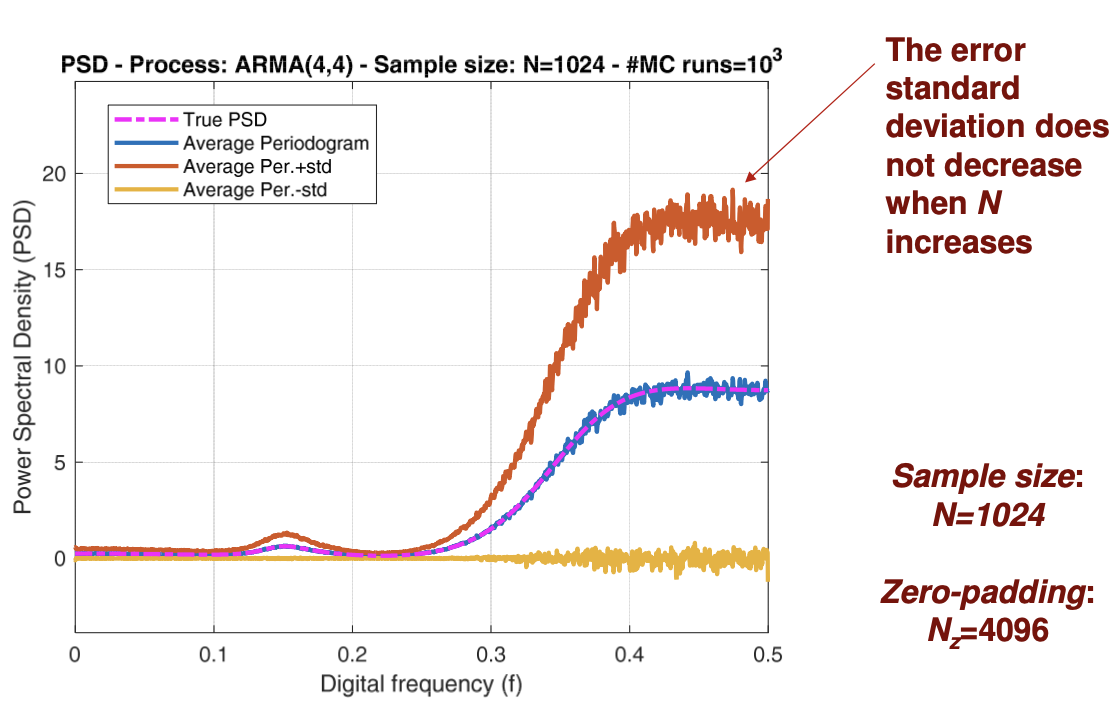
\includegraphics[width=0.65\linewidth]{Image/pdf 6/38.Periodo_N1024.png}
    \label{fig:placeholder}
\end{figure}
\item \textbf{Parametric estimation of the PSD}: we assume that the data can be modelled as an \underline{AR(P) process} of order P properly selected.
\item To identify the AR(P) model we first estimate the ACF values from lag \(m=0\) to lag \(m=P\) (with \(P\ll N\)) by using the unbiased sample estimator of the ACF by using an efficient algorithm, e.g. the \textbf{Levinson-Durbin algorithm}.
\[
\{X[n]\}_{n=0}^{N-1}\quad\Rightarrow\quad\{\hat{R}_X[m]\}_{m=0}^{P}\quad\Rightarrow\quad\{\hat{\sigma}_W^2,\mathbf{\hat{a}}\}
\]
\item Once we have estimated \textbf{a} and the power of \(W[n]\), we get the parametric estimate of the PSD, under the assumption that it is an AR(P) process.
\[
\hat{S}_X(e^{j2\pi f})=\frac{\hat{\sigma}_W^2}{\left|1-\sum_{k=1}^{P}\hat{a}e^{-j2\pi k f }\right|^2}
\]
\begin{figure}[H]
    \centering
    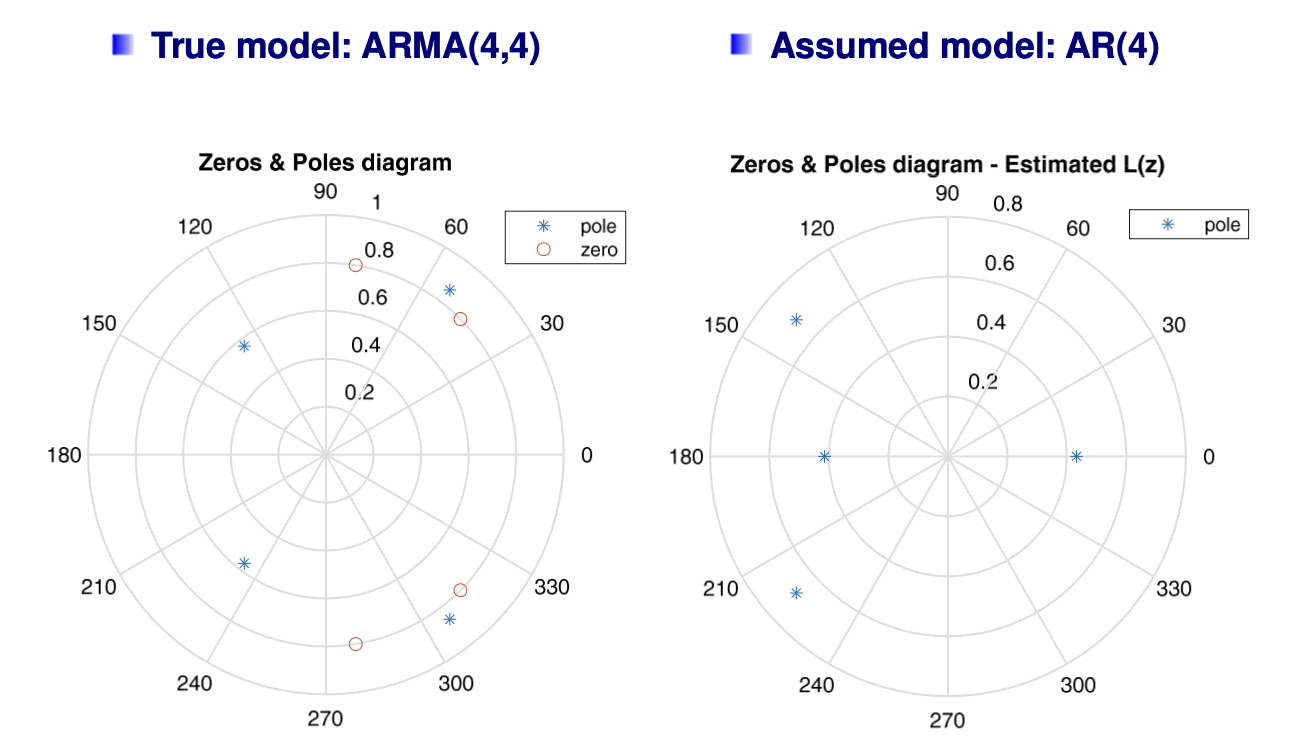
\includegraphics[width=0.65\linewidth]{Image/pdf 6/40.Zero_pole.png}
    \label{fig:placeholder}
\end{figure}
\begin{figure}[H]
    \centering
    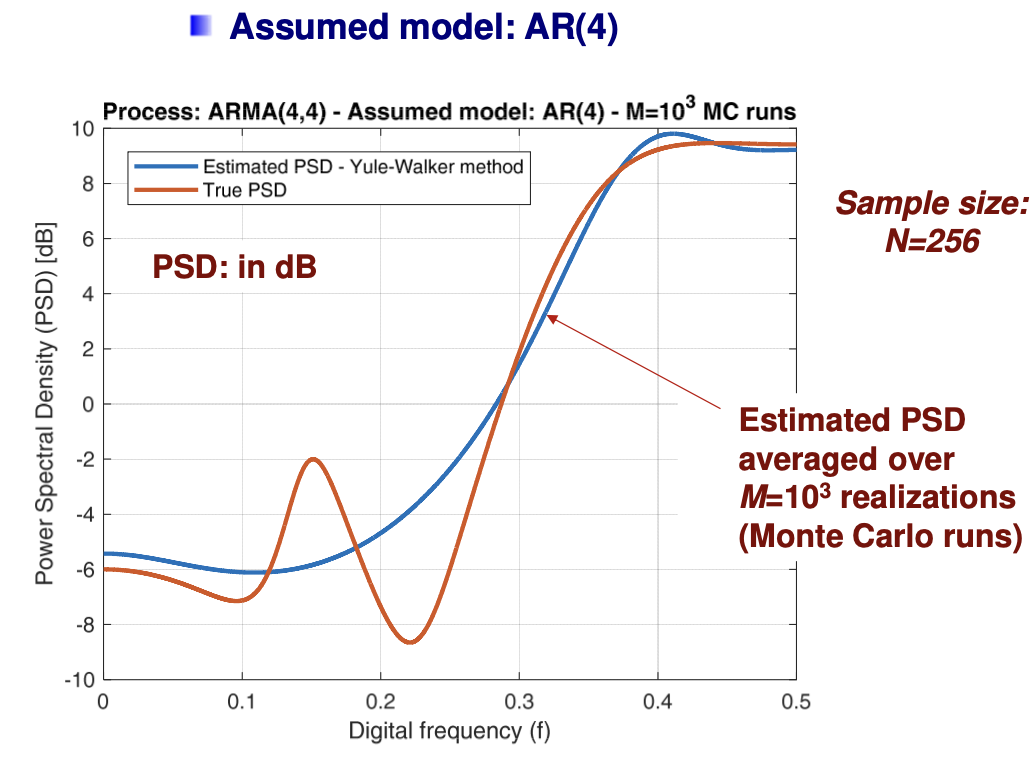
\includegraphics[width=0.65\linewidth]{Image/pdf 6/41.PSD_estimated.png}
    \label{fig:placeholder}
\end{figure}
\begin{figure}[H]
    \centering
    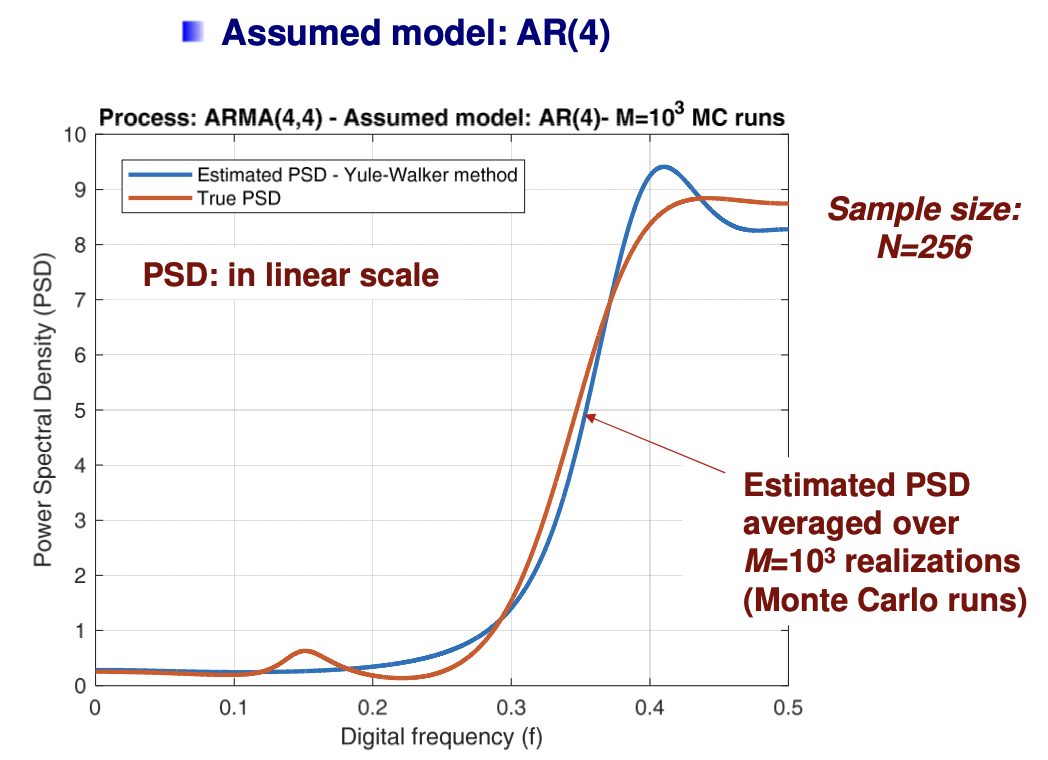
\includegraphics[width=0.65\linewidth]{Image/pdf 6/42.PSD_scaled.png}
    \label{fig:placeholder}
\end{figure}
\begin{figure}[H]
    \centering
    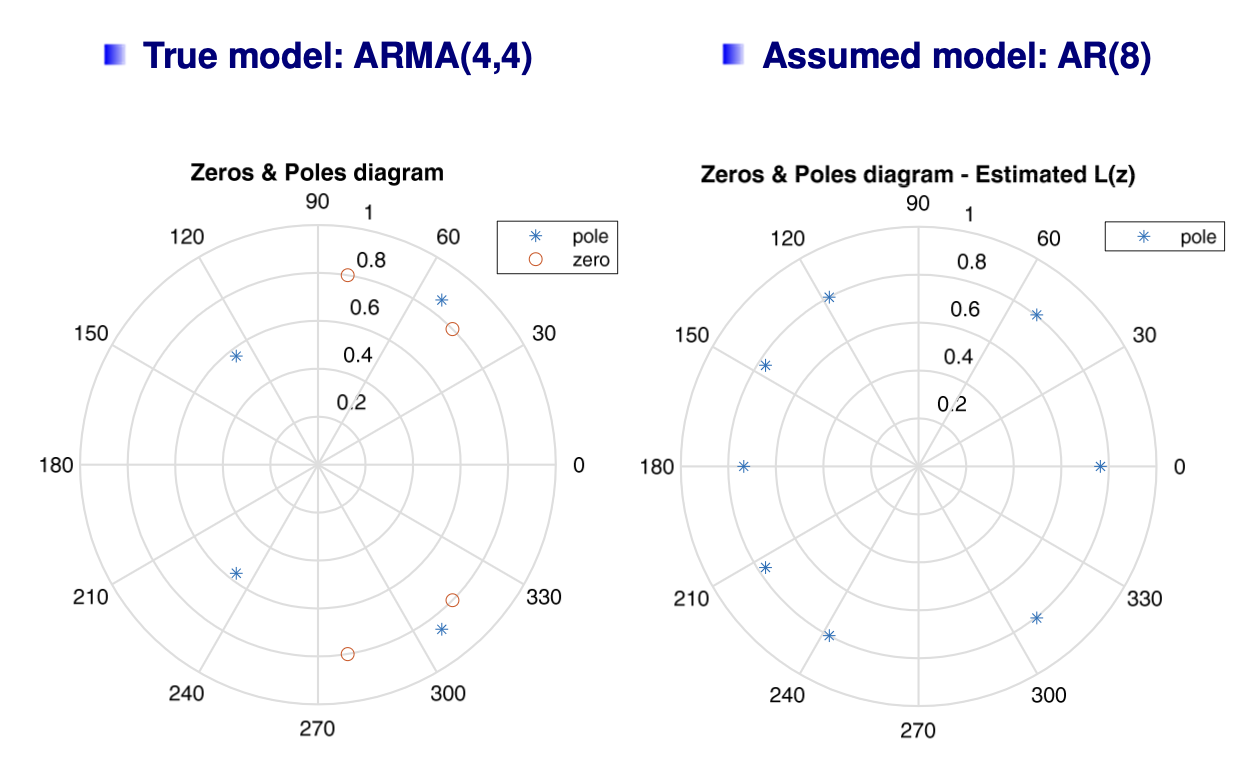
\includegraphics[width=0.65\linewidth]{Image/pdf 6/42.Zero_Pole_AR(8).png}
    \label{fig:placeholder}
\end{figure}
\begin{figure}[H]
    \centering
    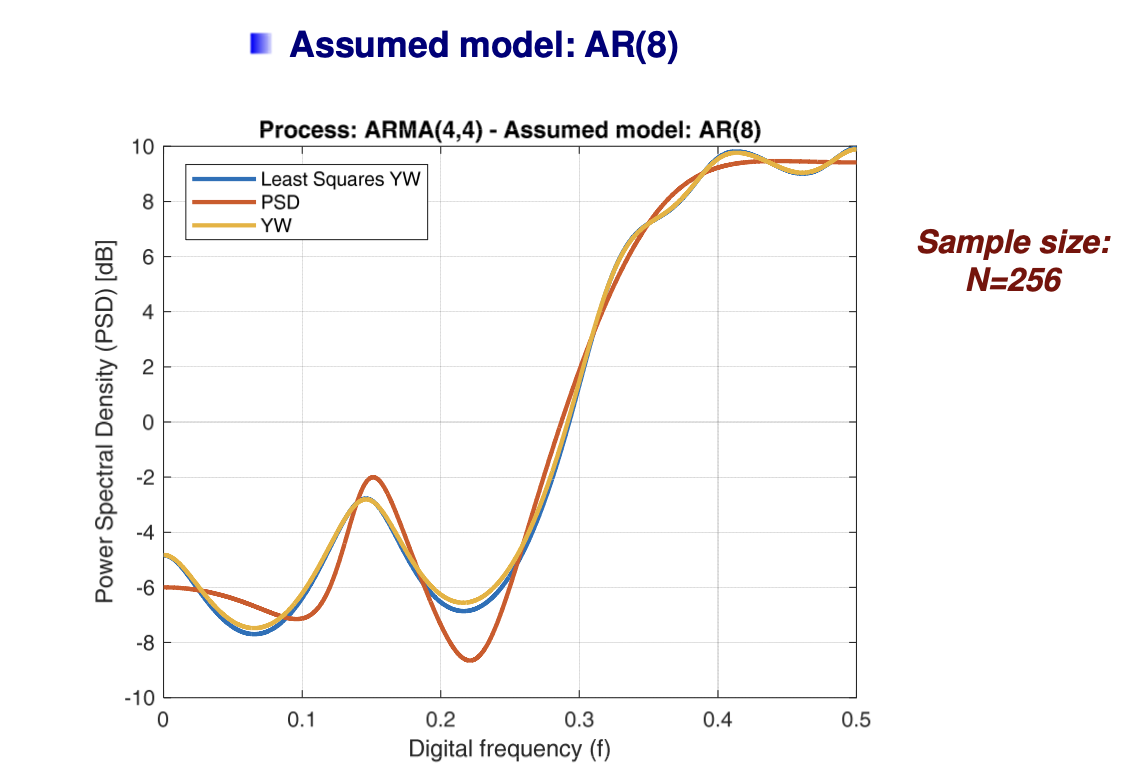
\includegraphics[width=0.65\linewidth]{Image/pdf 6/43.PSD_AR(8).png}
    \label{fig:placeholder}
\end{figure}
\begin{figure}[H]
    \centering
    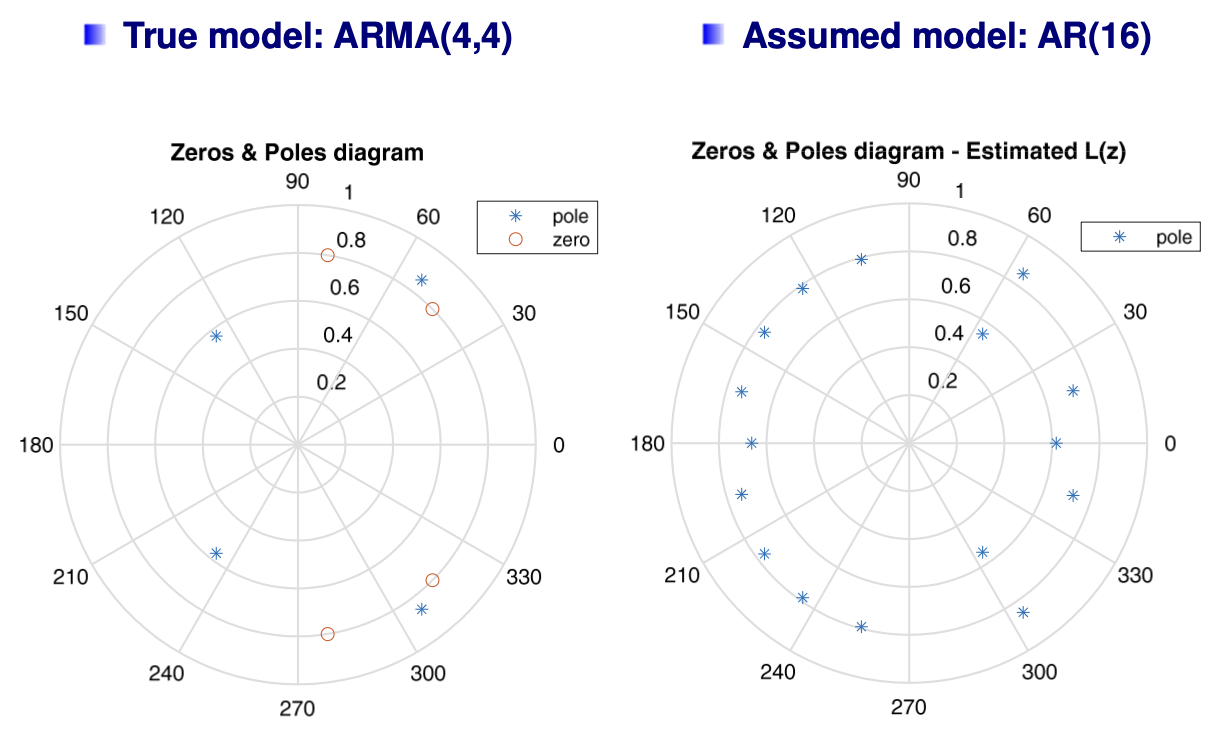
\includegraphics[width=0.65\linewidth]{Image/pdf 6/44.Zero_pole_AR(16).png}
    \label{fig:placeholder}
\end{figure}
\begin{figure}[H]
    \centering
    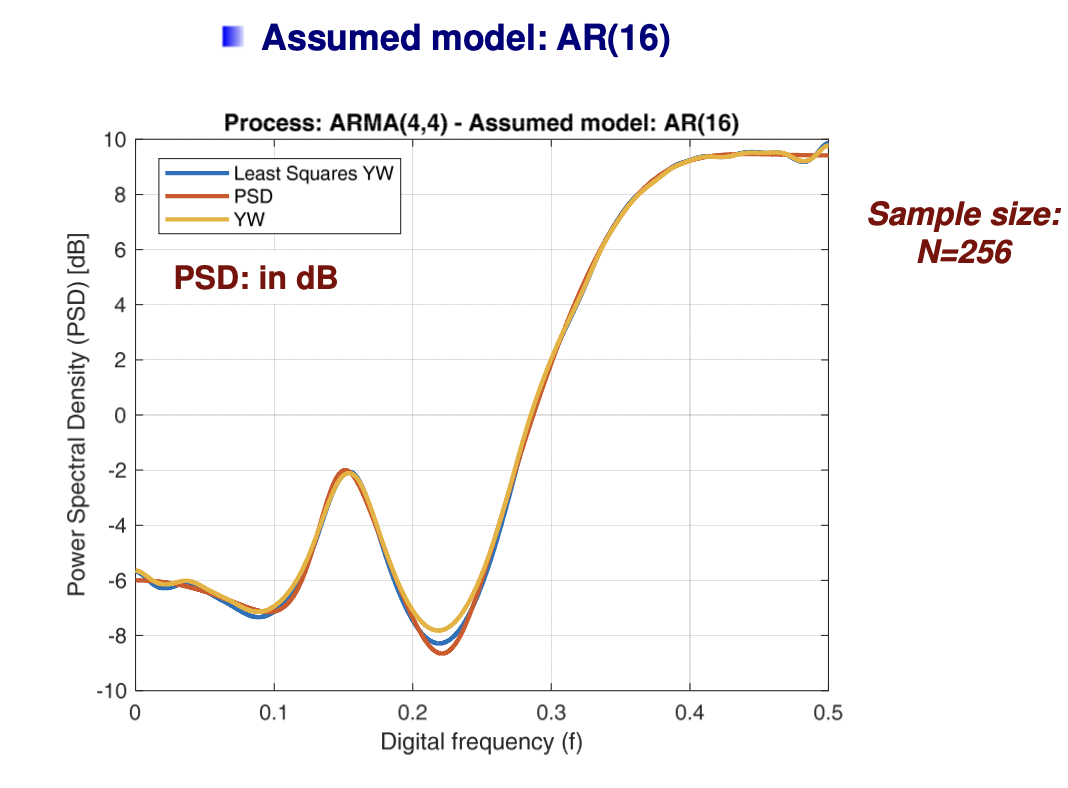
\includegraphics[width=0.65\linewidth]{Image/pdf 6/45.PSD_assumed_AR(16).png}
    \label{fig:placeholder}
\end{figure}
\item \textbf{Example}: let us consider the following \textbf{narrowband ARMA(4,2) process} whose innovation filter has a system function:
\begin{align*}
H(z) = \frac{B(z)}{A(z)}
&=
\frac{1 + 1.5857 z^{-1} + 0.9604 z^{-2}}
     {1 - 1.6408 z^{-1} + 2.2044 z^{-2} - 1.4808 z^{-3} + 0.8145 z^{-4}}
\end{align*}
\begin{figure}[H]
    \centering
    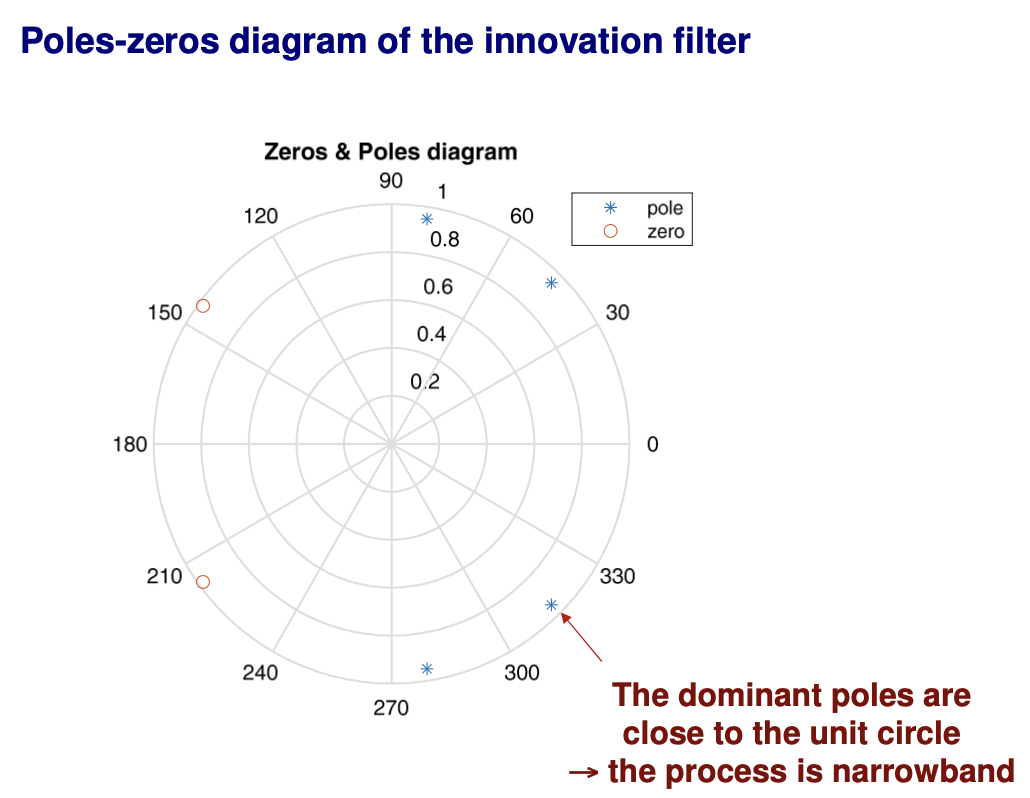
\includegraphics[width=0.65\linewidth]{Image/pdf 6/46.Zero_pole.png}
    \label{fig:placeholder}
\end{figure}
\begin{figure}[H]
    \centering
    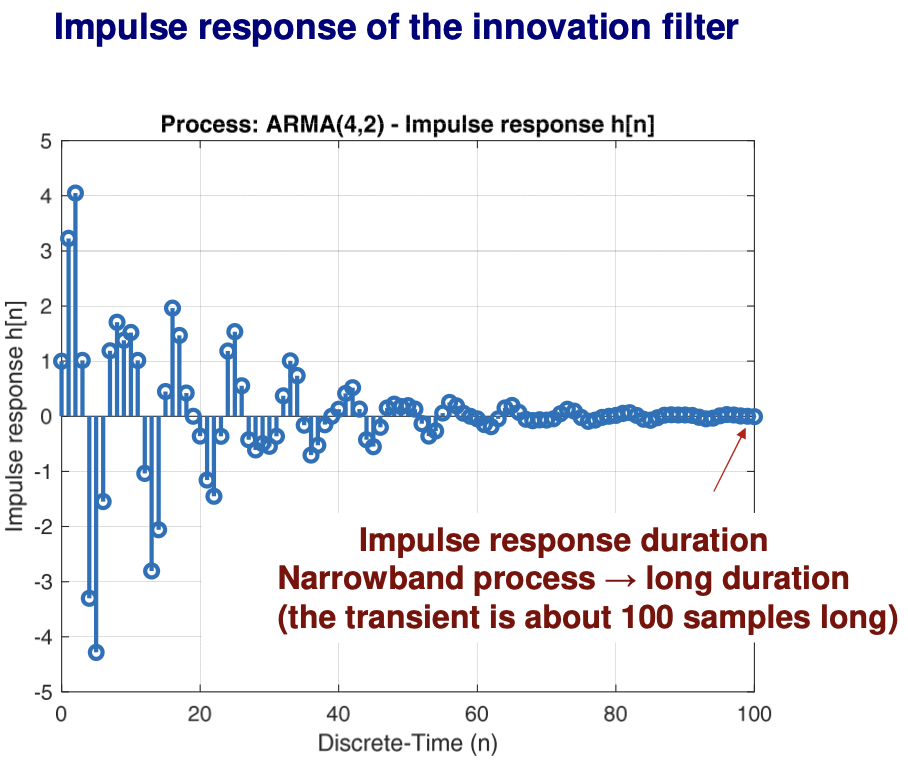
\includegraphics[width=0.65\linewidth]{Image/pdf 6/47.Impulse_response.png}
    \label{fig:placeholder}
\end{figure}
\begin{figure}[H]
    \centering
    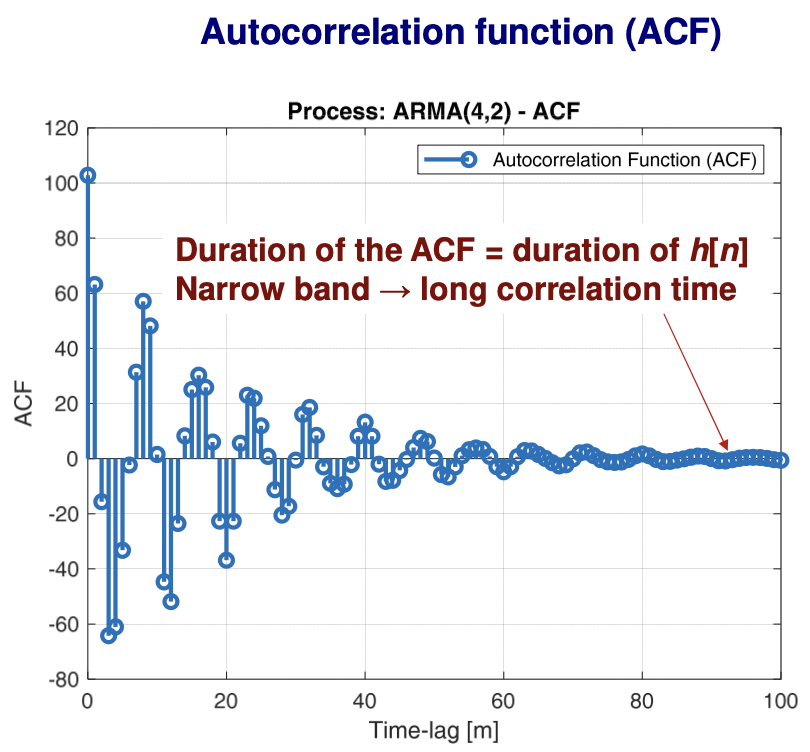
\includegraphics[width=0.65\linewidth]{Image/pdf 6/48.ACF.png}
    \label{fig:placeholder}
\end{figure}
\begin{figure}[H]
    \centering
    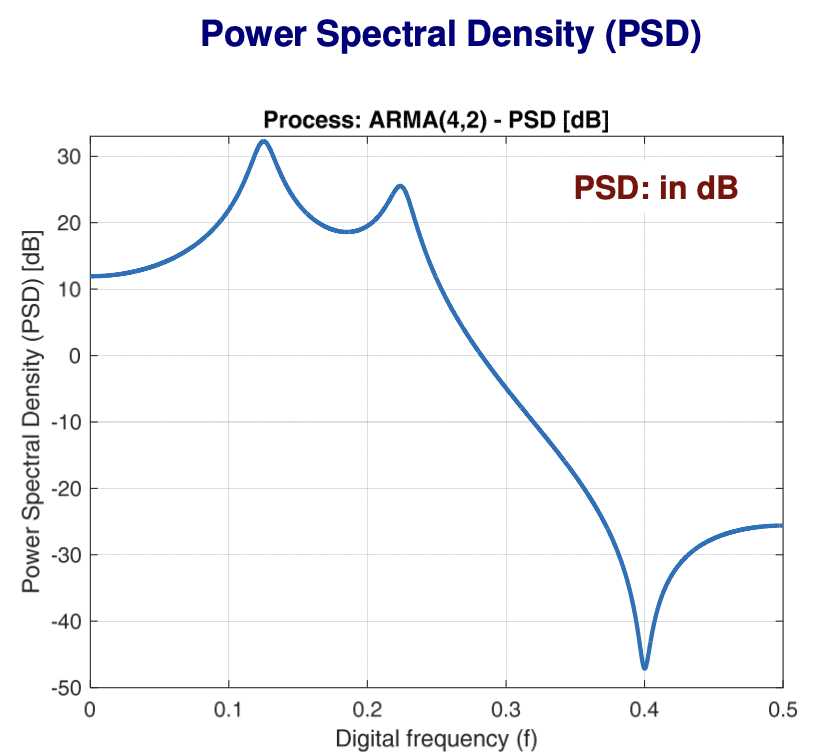
\includegraphics[width=0.65\linewidth]{Image/pdf 6/49.PSD.png}
    \label{fig:placeholder}
\end{figure}
\begin{figure}[H]
    \centering
    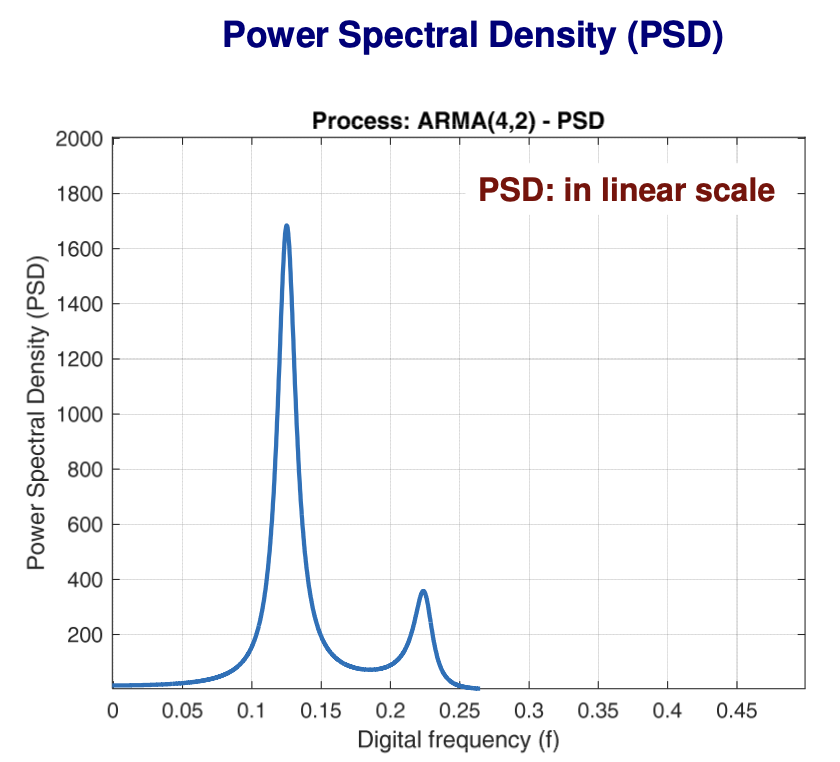
\includegraphics[width=0.65\linewidth]{Image/pdf 6/50.PSD_lin.png}
    \label{fig:placeholder}
\end{figure}
\begin{figure}[H]
    \centering
    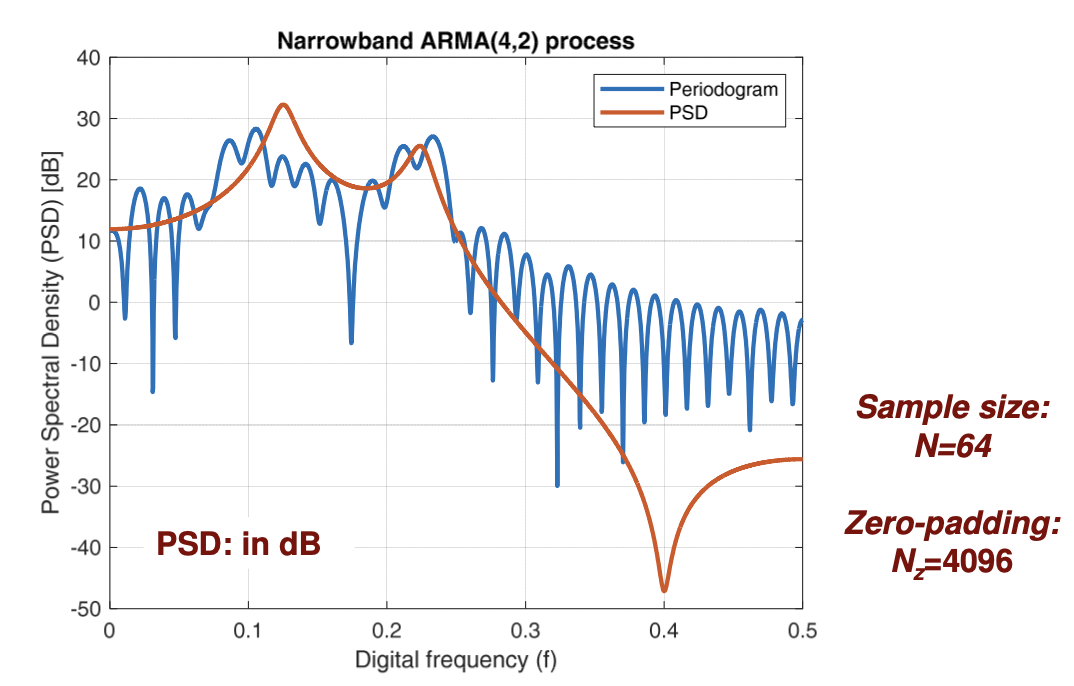
\includegraphics[width=0.65\linewidth]{Image/pdf 6/51.PSD_N64.png}
    \label{fig:placeholder}
\end{figure}
\begin{figure}[H]
    \centering
    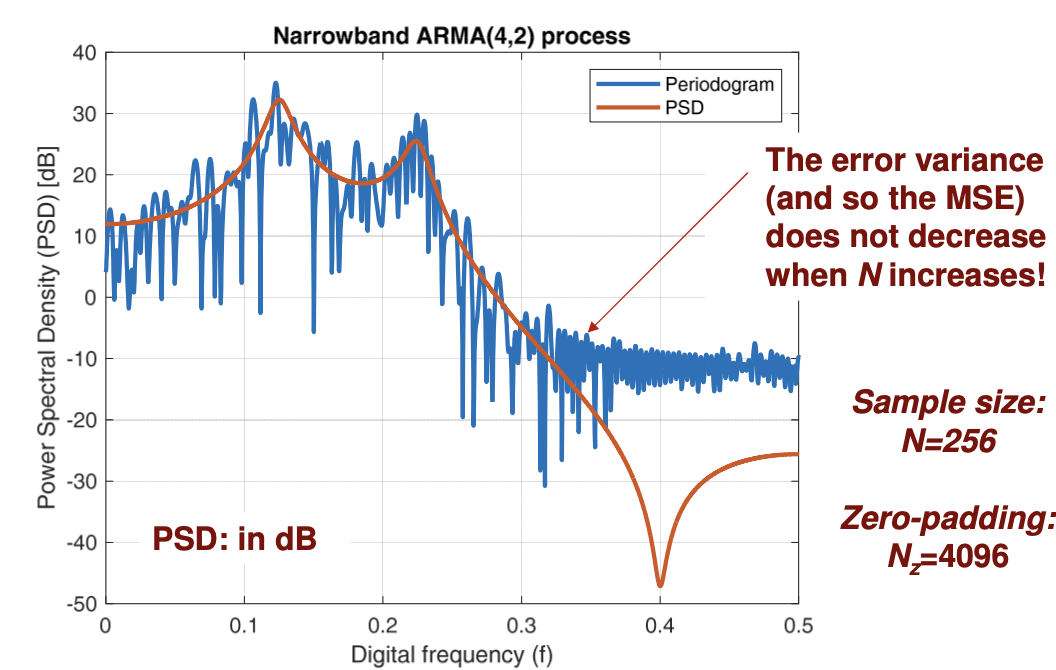
\includegraphics[width=0.65\linewidth]{Image/pdf 6/52.PSD_N256.png}
    \label{fig:placeholder}
\end{figure}
\begin{figure}[H]
    \centering
    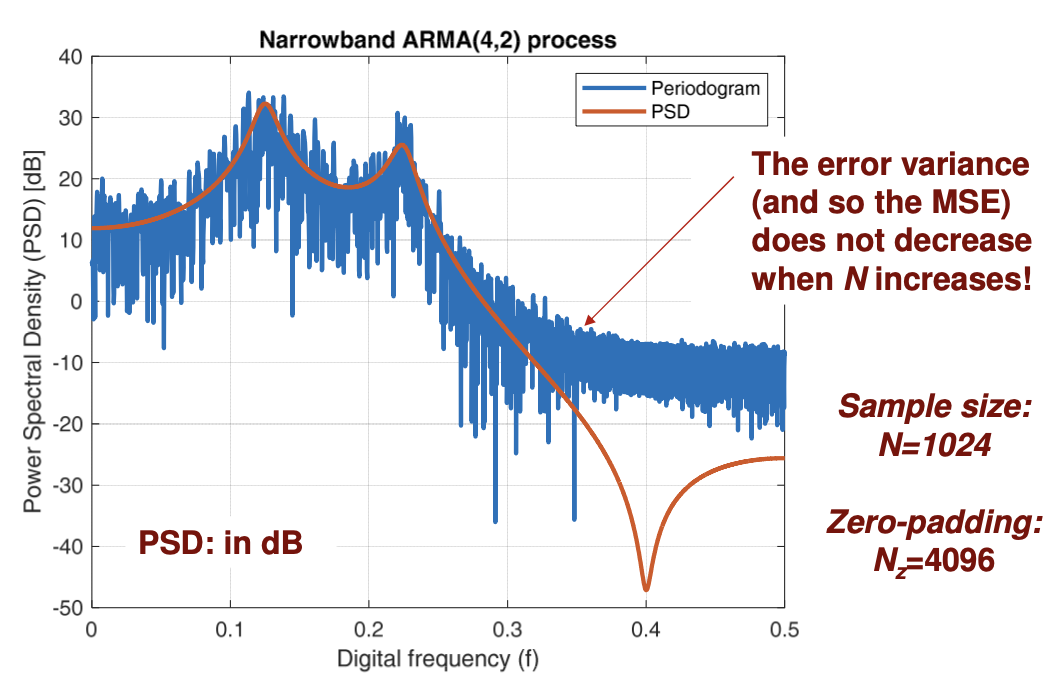
\includegraphics[width=0.65\linewidth]{Image/pdf 6/53.PSD_N1024.png}
    \label{fig:placeholder}
\end{figure}
\begin{figure}[H]
    \centering
    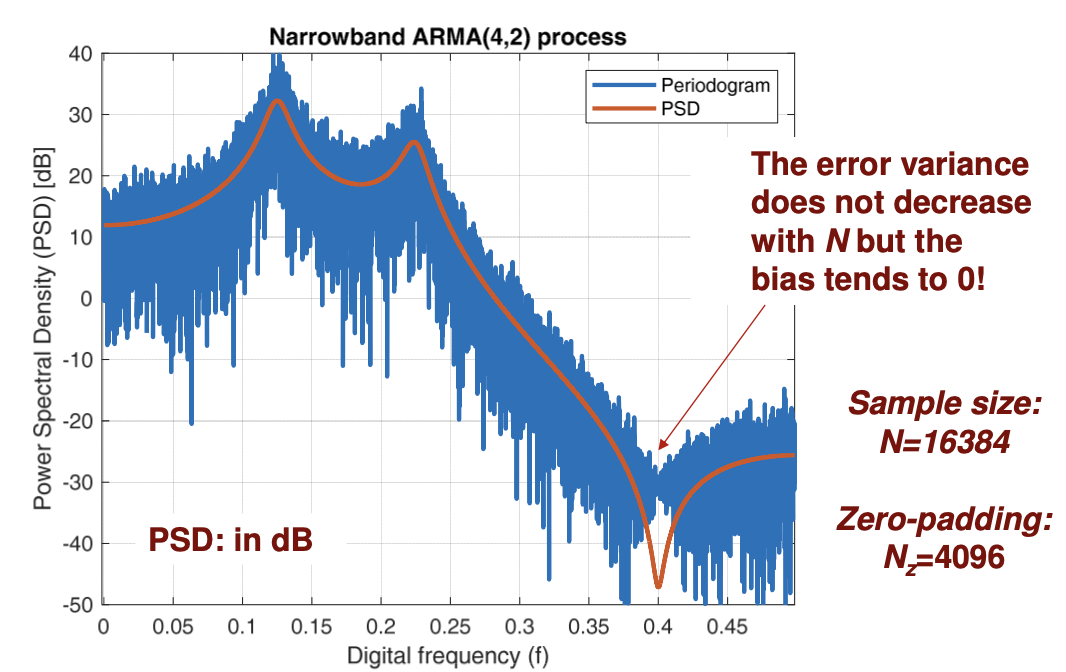
\includegraphics[width=0.65\linewidth]{Image/pdf 6/54.PSD_N16384.png}
    \label{fig:placeholder}
\end{figure}
\begin{figure}[H]
    \centering
    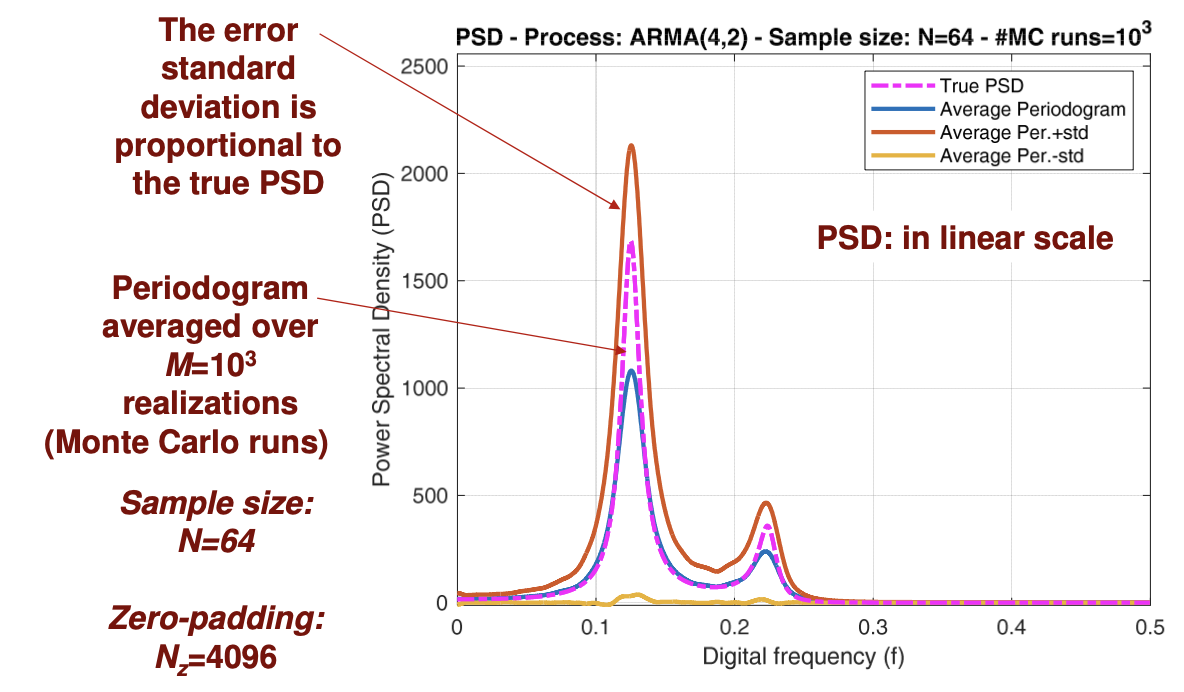
\includegraphics[width=0.65\linewidth]{Image/pdf 6/55.Periodo_N64.png}
    \label{fig:placeholder}
\end{figure}
\begin{figure}[H]
    \centering
    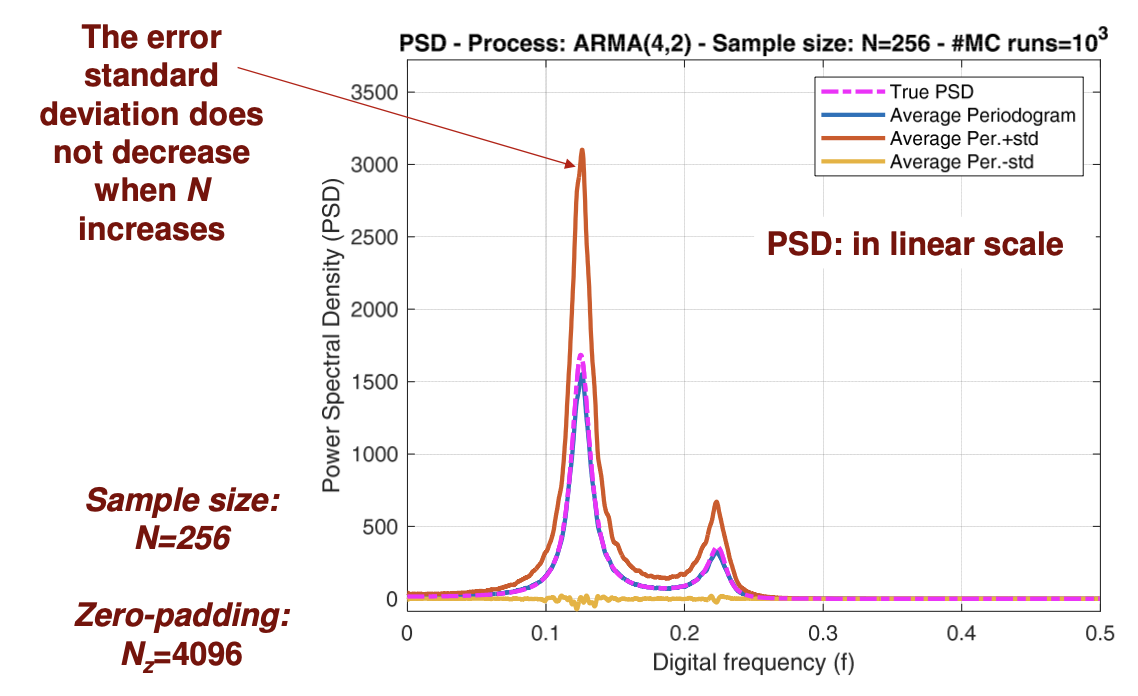
\includegraphics[width=0.65\linewidth]{Image/pdf 6/56.Periodo_N256.png}
    \label{fig:placeholder}
\end{figure}
\begin{figure}[H]
    \centering
    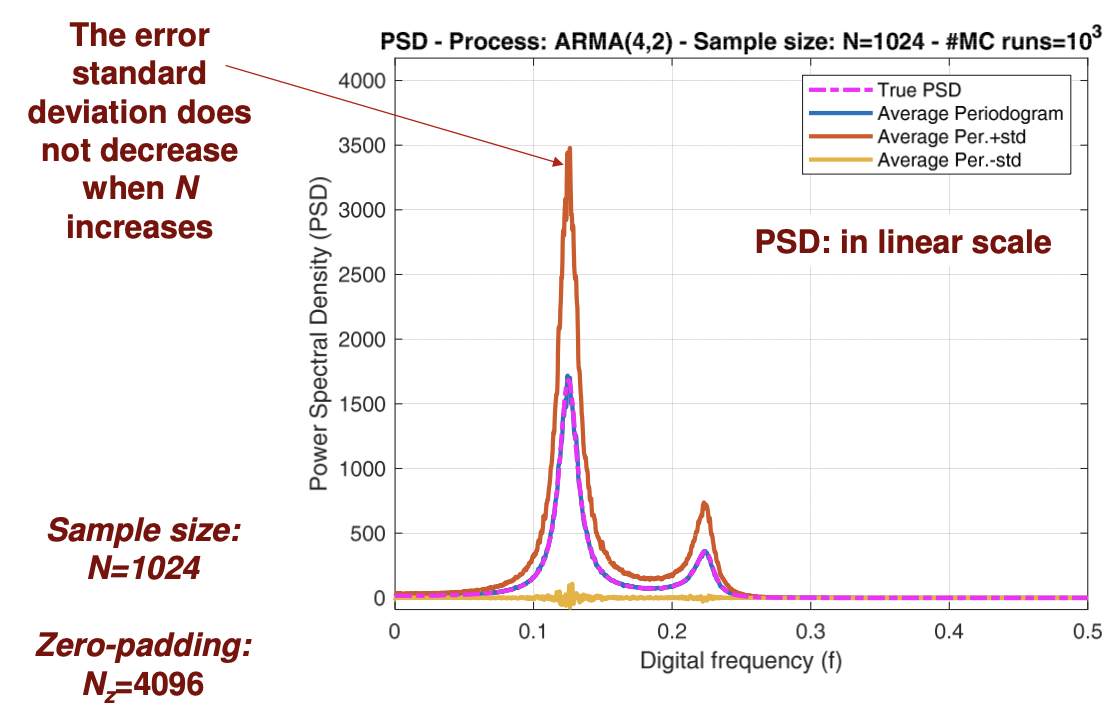
\includegraphics[width=0.65\linewidth]{Image/pdf 6/57.Periodo_N1024.png}
    \label{fig:placeholder}
\end{figure}
\begin{figure}[H]
    \centering
    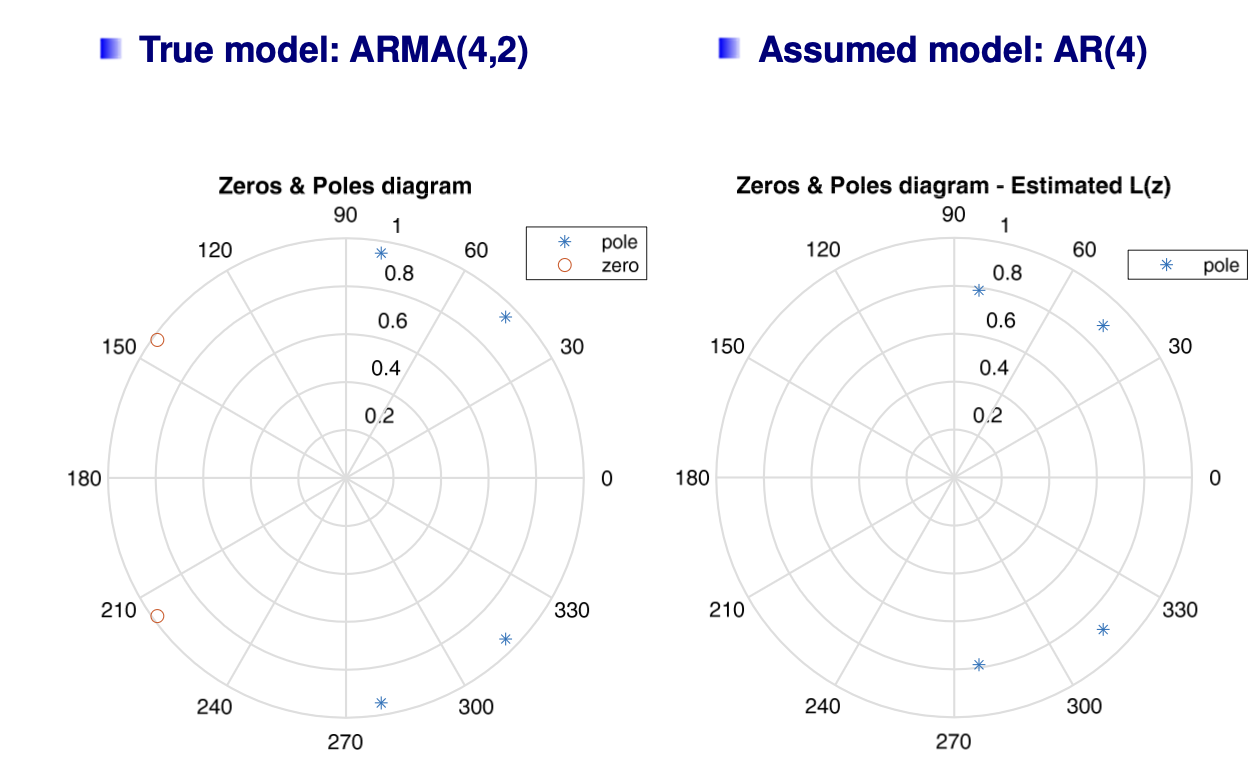
\includegraphics[width=0.65\linewidth]{Image/pdf 6/58.Assumed_AR(4).png}
    \label{fig:placeholder}
\end{figure}
\begin{figure}[H]
    \centering
    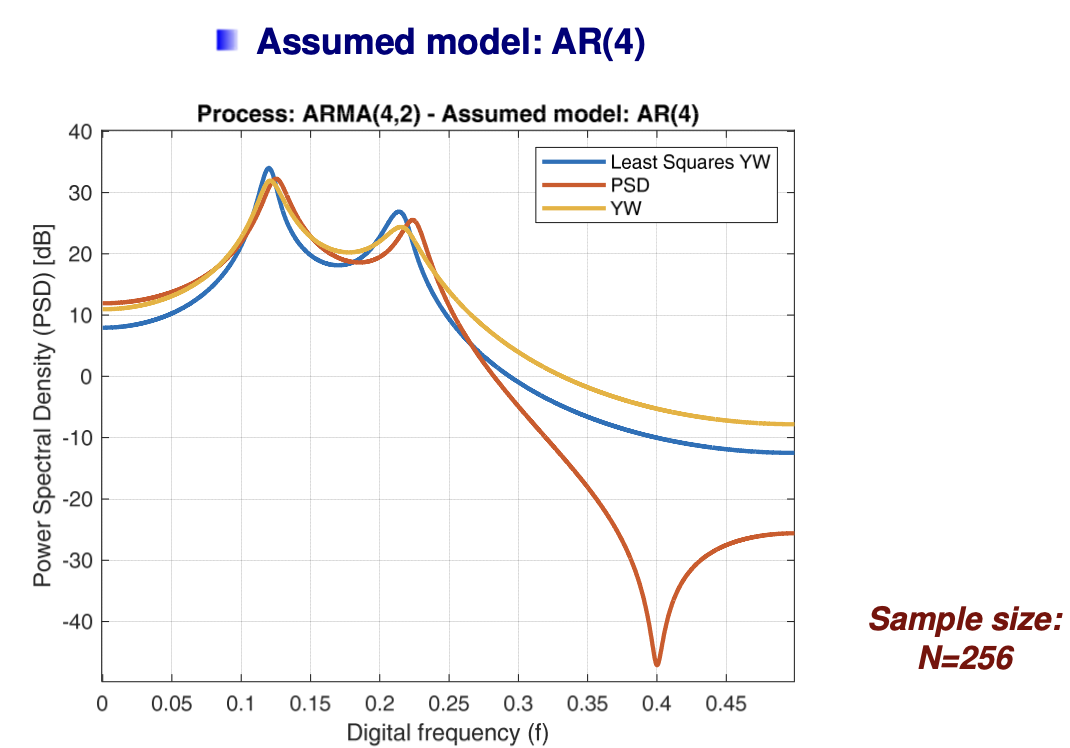
\includegraphics[width=0.65\linewidth]{Image/pdf 6/59.PSD_AR(4).png}
    \label{fig:placeholder}
\end{figure}
\begin{figure}[H]
    \centering
    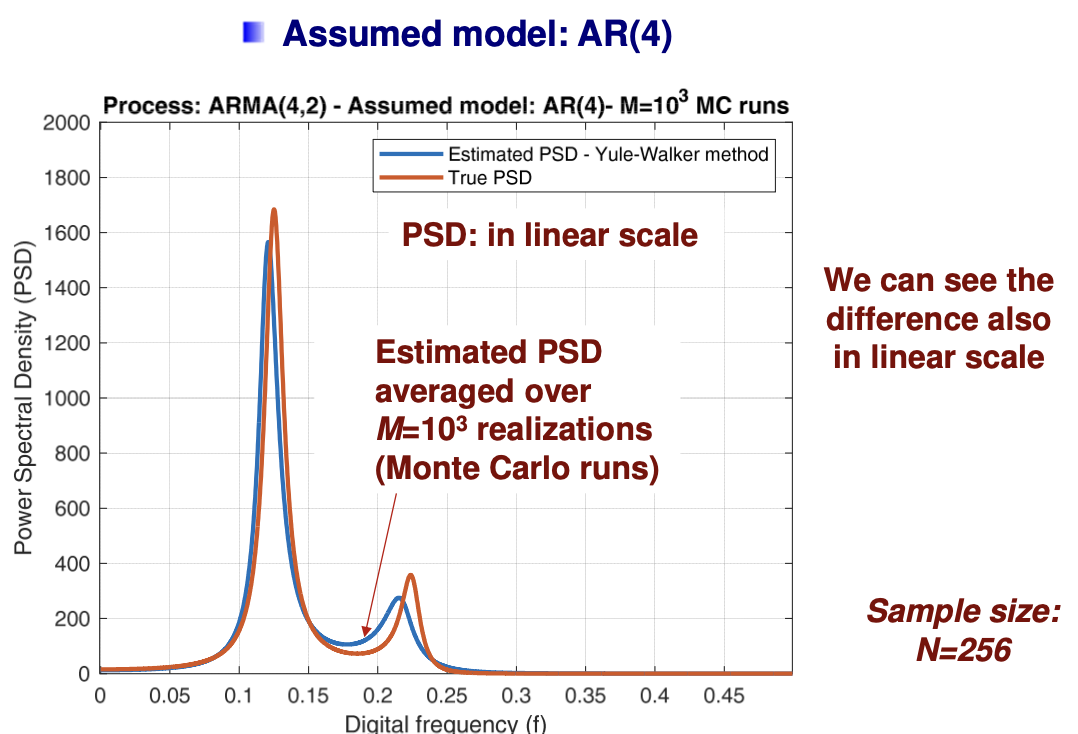
\includegraphics[width=0.65\linewidth]{Image/pdf 6/60.PSD2_AR(4).png}
    \label{fig:placeholder}
\end{figure}
\begin{figure}[H]
    \centering
    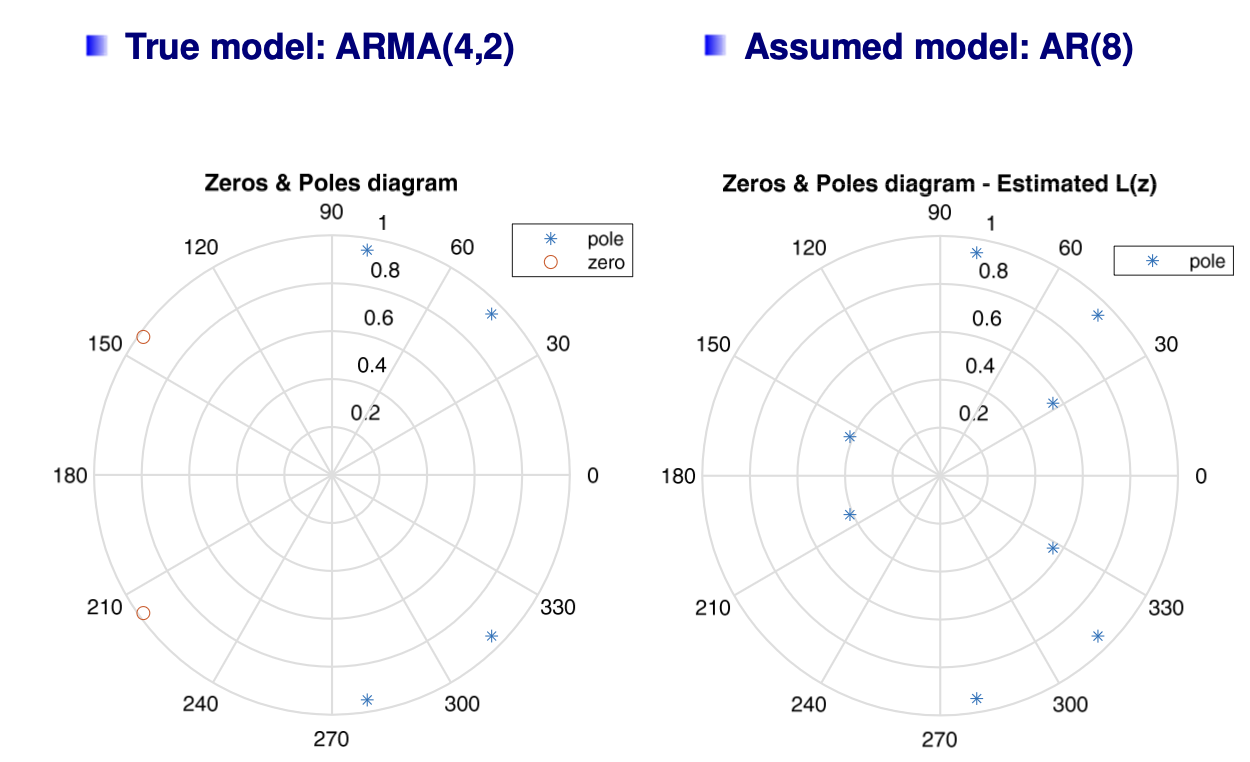
\includegraphics[width=0.65\linewidth]{Image/pdf 6/61.Assumed_AR(8).png}
    \label{fig:placeholder}
\end{figure}
\begin{figure}[H]
    \centering
    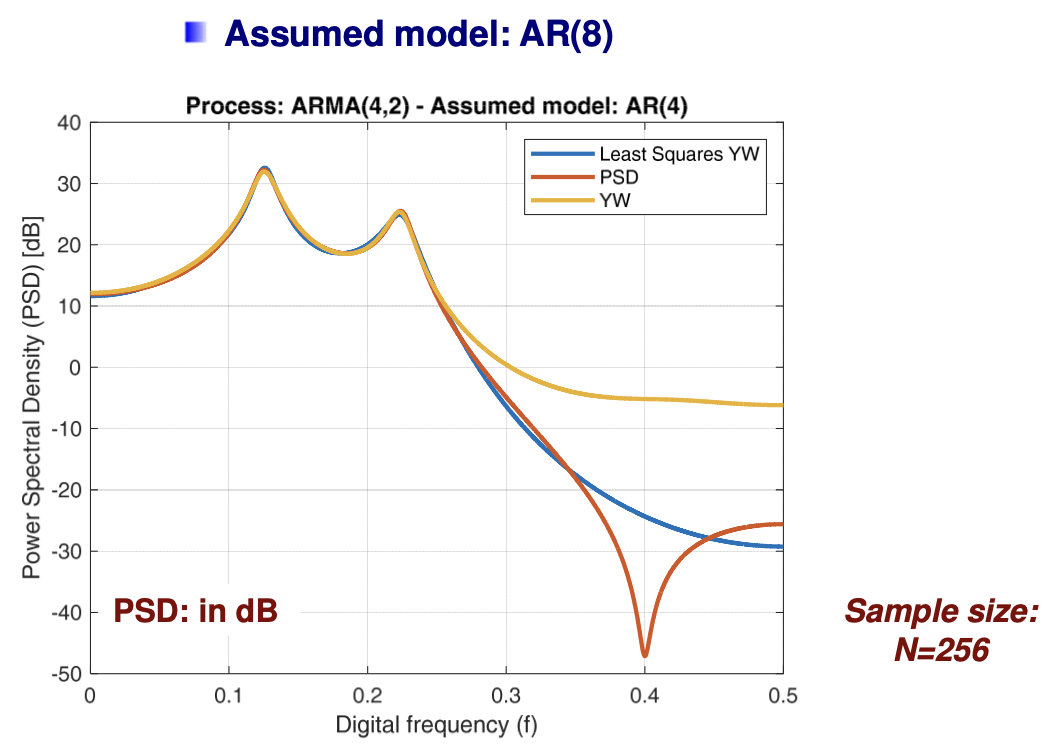
\includegraphics[width=0.65\linewidth]{Image/pdf 6/62.PSD_AR(8).png}
    \label{fig:placeholder}
\end{figure}
\begin{figure}[H]
    \centering
    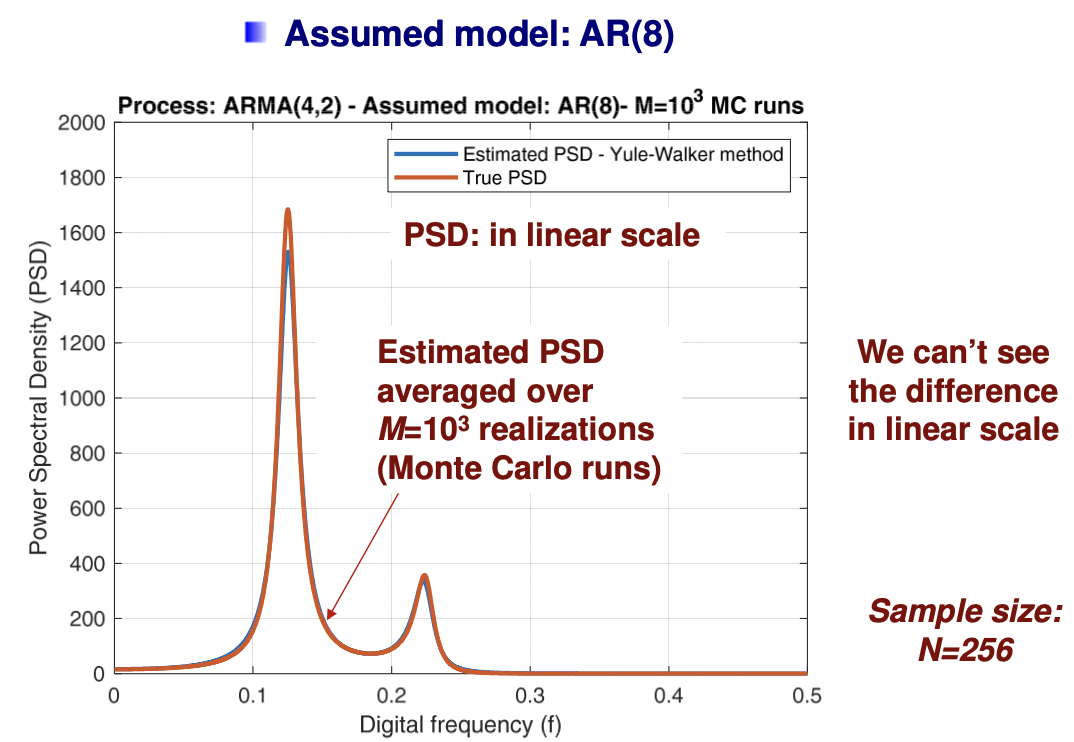
\includegraphics[width=0.65\linewidth]{Image/pdf 6/63.PSD2_AR(8).png}
    \label{fig:placeholder}
\end{figure}
\begin{figure}[H]
    \centering
    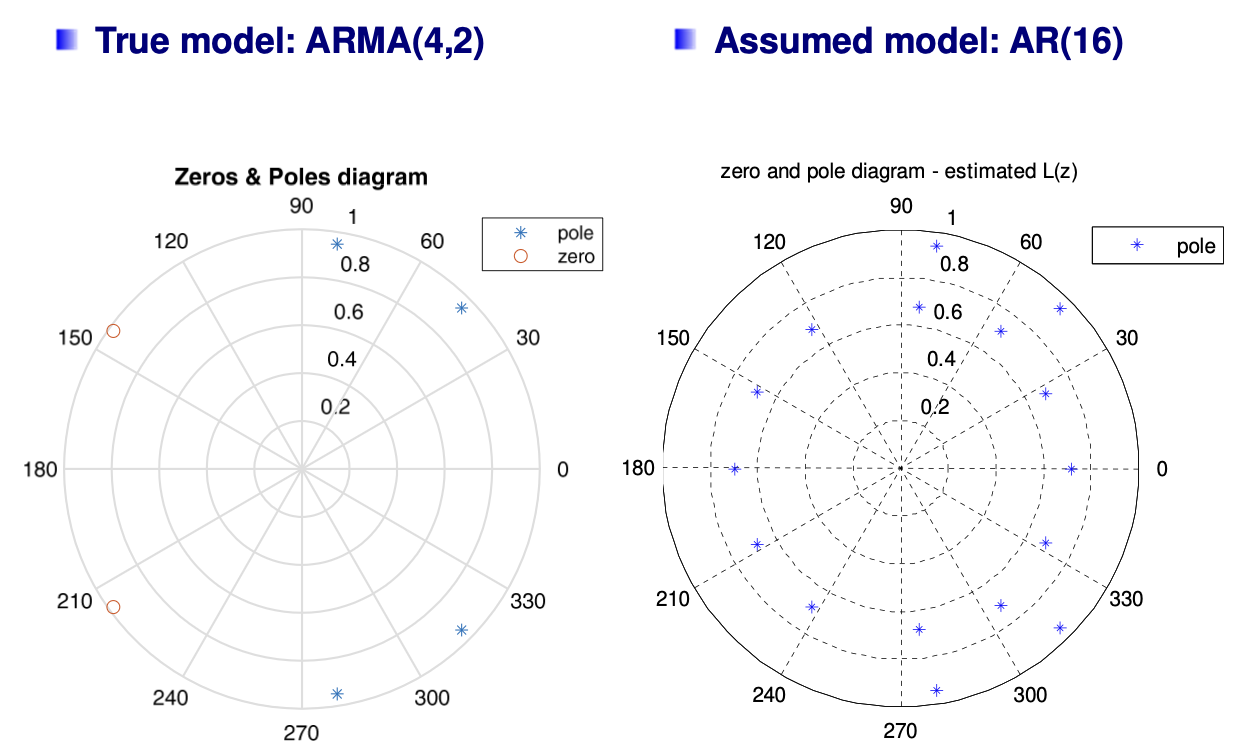
\includegraphics[width=0.65\linewidth]{Image/pdf 6/64.Assumed_AR(16).png}
    \label{fig:placeholder}
\end{figure}
\begin{figure}[H]
    \centering
    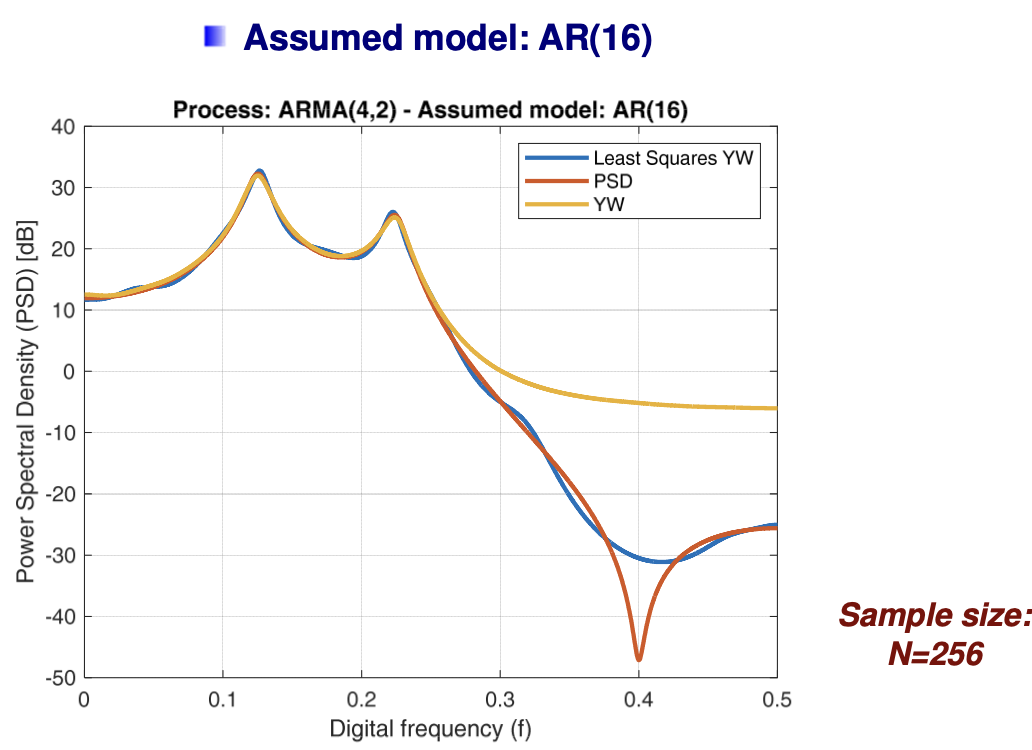
\includegraphics[width=0.65\linewidth]{Image/pdf 6/65.PSD_AR(16).png}
    \label{fig:placeholder}
\end{figure}
\begin{figure}[H]
    \centering
    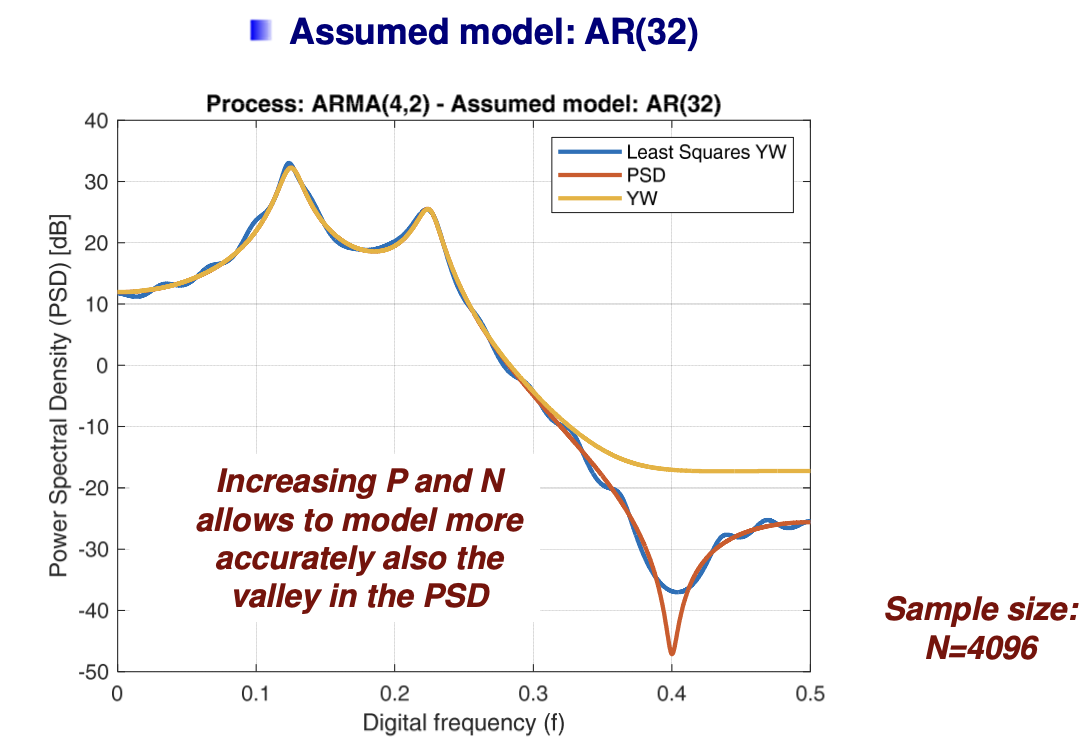
\includegraphics[width=0.65\linewidth]{Image/pdf 6/66.AR(32).png}
    \label{fig:placeholder}
\end{figure}
\end{itemize}

